\documentclass[11pt,a4paper]{article}
\usepackage[spanish,es-noshorthands,es-tabla]{babel}
\usepackage[utf8]{inputenc}\usepackage[T1]{fontenc}\usepackage{lmodern}
\usepackage[margin=2.2cm]{geometry}\usepackage{graphicx}\usepackage{booktabs}\usepackage{amsmath}\usepackage{float}\usepackage{xcolor}
\usepackage{adjustbox}\usepackage{xurl}\usepackage[colorlinks=true,linkcolor=blue!50!black,urlcolor=blue!50!black]{hyperref}
\usepackage{caption}\captionsetup{font=small,labelfont=bf}\usepackage{pdflscape}\usepackage{longtable}\usepackage{colortbl}
\newcommand{\aviso}[1]{\begin{center}\fcolorbox{orange!70!black}{orange!6}{\parbox{0.93\linewidth}{\small #1}}\end{center}}
\sloppy
\title{Réplica de Sidelnik et al. (2020) en MEIGA \\ \large Neutrones de 500\,MeV horizontales en el WCD de acero: Agua pura, 2,5\,\% NaCl, 5\,\% NaCl, 10\,\% NaCl}
\author{Informe técnico preparado para Jaime Betancourt}
\date{13 de octubre de 2026}
\begin{document}\maketitle
\begin{abstract}
Se analizan las corridas de MEIGA preparadas para la Sec.~4.1.1 de la tesis: 150\,000 neutrones de 500\,MeV que entran horizontalmente,
a media altura, a un WCD de 96\,cm $\times$ 133\,cm con Tyvek de 0,12\,mm, acero de 0,5\,mm y el PMT en la tapa, sin dispersión térmica $S(\alpha,\beta)$.
Se comparan con la Tabla~2 y las Figs.~2--6 de Sidelnik et al., \textit{Adv. Space Res.} 65 (2020) 2216.
Este informe se regenera automáticamente cuando se agregan los demás medios.
\end{abstract}
\tableofcontents

\section{Configuración de la simulación}
{\small\textit{Corresponde a la Sec.~4.1.1.1 de la tesis (Tabla 4.1).}}

\subsection{Parámetros de la simulación}
\begin{table}[H]\centering\small\begin{adjustbox}{max width=\linewidth}\begin{tabular}{ll}\toprule
Parámetro & Valor en MEIGA (igual que en Sidelnik et al.\ 2020) \\\midrule
Tanque & cilindro de agua de 48\,cm de radio y 133\,cm de altura \\
Paredes & Tyvek de 0,12\,mm y acero inoxidable de 0,5\,mm (lados, tapa y fondo) \\
Fotomultiplicador & 10,16 $\times$ 10,16 $\times$ 5\,cm, en la tapa \\
Medios & agua pura; agua + 2,5, 5 y 10\,\% NaCl (Ec.~3.12; densidad y $n$ de la Tabla~3.6) \\
Fuente & neutrones de 500\,MeV, horizontales, a media altura (66,562\,cm), 1\,cm fuera de la pared \\
Neutrones por medio & 150\,000 \\
Física & Geant4 10.7.p04, \texttt{QGSP\_BERT\_HP\_NoThermal} (sin $S(\alpha,\beta)$), G4NDL\,4.6 \\
Óptica & modo \texttt{eFast}: eficiencia cuántica del R5912 aplicada al crearse cada fotón \\\bottomrule
\end{tabular}\end{adjustbox}\caption{Parámetros de las corridas (equivalente a la Tabla~4.1 de la tesis).}\end{table}
\begin{figure}[H]\centering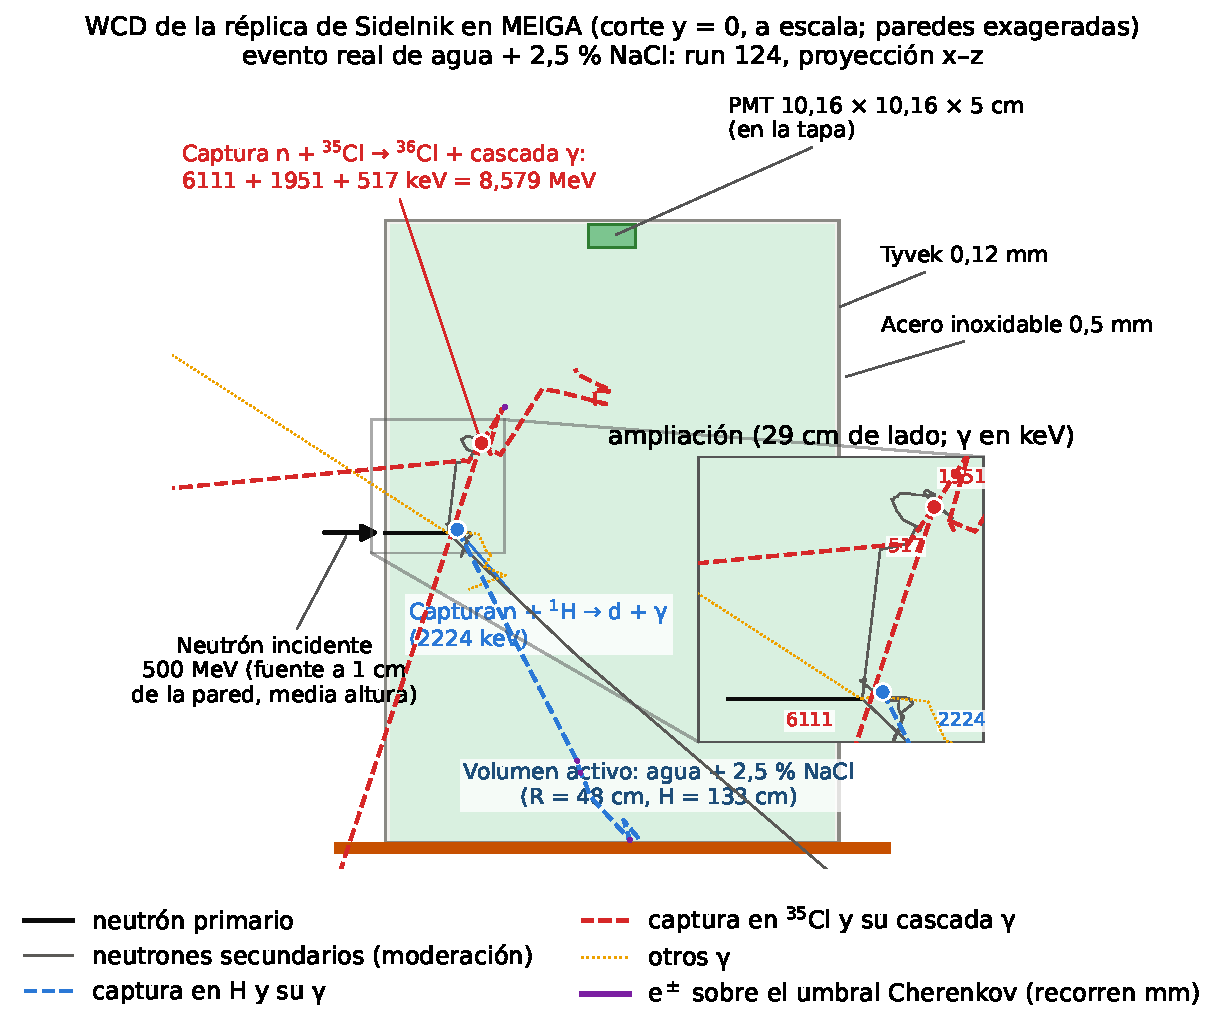
\includegraphics[width=0.92\linewidth]{../figuras/fig00_esquema_detector.pdf}\caption{Esquema del WCD simulado (corte $y = 0$, a escala; el espesor de las paredes está exagerado) con un evento real de la corrida de agua + 2,5\,\% NaCl (\texttt{run\_id} 124):
el neutrón de 500\,MeV entra a media altura y tiene una interacción inelástica; los neutrones secundarios se moderan y dos de ellos se capturan, uno en $^1$H (gamma de 2224\,keV, azul) y otro en $^{35}$Cl,
con la cascada 6111 + 1951 + 517\,keV que conserva la energía de separación (8,579\,MeV; rojo; véase el esquema de niveles de la Sec.~\ref{sec:esquemas}). Los electrones de los gammas (violeta) recorren pocos milímetros y emiten la luz Cherenkov.
Equivalente a la Fig.~1 de Sidelnik et al.\ (2020), pero con la geometría y las trayectorias de MEIGA. La versión de agua pura (captura en H) está en \texttt{figuras/fig00\_esquema\_detector\_pura}.}\label{fig:esquema}\end{figure}
\subsection{Corridas analizadas}
Corrida de agua pura: \url{Corridas-Sidelnik-500MeV/150000N-500MeV-Sidelnik-H2O-pura-sinSab-20261012-061022} (disco ADATA, 124\,GB, 20,2\,h de cómputo).
Cada neutrón primario es una corrida de MEIGA (\texttt{run\_id} 0--149\,999); la carga de \texttt{Carga-total.txt} coincide evento por evento con \texttt{output.json.gz}.
Se leyeron todos los archivos salvo \texttt{pasos-particulas.tsv} (78\,GB), que no se necesita para estos observables.
\par Corrida de agua + 2,5\,\% NaCl, en dos tramos: \url{42649N-parcial-500MeV-Sidelnik-H2O-2.5NaCl-sinSab-20261013} (43\,GB), interrumpida al detenerse el contenedor (se usan los 42\,649 neutrones terminados y se descartan las filas del incompleto),
y su complemento \url{107351N-500MeV-Sidelnik-H2O-2.5NaCl-sinSab-20261013-135213} (108\,GB, 16,6\,h), lanzado con otra semilla (MEIGA la toma de la hora). Los dos tramos se unen en 150\,000 neutrones (\texttt{unir\_tramos.py}: los números de evento del complemento se desplazan en 42\,649 y los histogramas se suman);
sus resultados son compatibles dentro del error (neutrones con al menos una captura: $43{,}42\pm0{,}24$ y $43{,}25\pm0{,}15$\,\%; carga media: $11{,}45\pm0{,}15$ y $11{,}35\pm0{,}09$\,p.e.).
\par Corrida de agua + 5\,\% NaCl: \url{150000N-500MeV-Sidelnik-H2O-5NaCl-sinSab-20261014-065724} (162\,GB, 24,4\,h de cómputo).
\par Corrida de agua + 10\,\% NaCl: \url{150000N-500MeV-Sidelnik-H2O-10NaCl-sinSab-20261015-081303} (166\,GB, 26,8\,h de cómputo).


\section{Contribución de los principales núcleos a la captura de neutrones}
{\small\textit{Corresponde a la Sec.~4.1.1.2 de la tesis (Figs. 4.1 y 4.2, Tabla 4.2).}}

\subsection{Interacciones del neutrón primario}\label{sec:primario}
Antes de la captura conviene seguir al neutrón de 500\,MeV (la traza 1 de Geant4; \texttt{inelasticas\_primario.py}, que lee \texttt{interacciones-neutrones.tsv} y \texttt{secundarias-inelastica-neutron.tsv}).
El núcleo blanco de cada inelástica se deduce por conservación de la carga y del número bariónico de los productos; los isótopos $^{17}$O (0,04\,\%) y $^{18}$O (0,21\,\%) aparecen con su abundancia natural, lo que valida la reconstrucción.
\begin{table}[H]\centering\small\begin{adjustbox}{max width=\linewidth}\begin{tabular}{lcccc}\toprule
Destino del neutrón primario & Agua pura & 2,5\,\% & 5\,\% & 10\,\% \\\midrule
Atraviesa el tanque sin interactuar & 21,8\,\% & 21,3\,\% & 21,0\,\% & 20,0\,\% \\
Interacción inelástica (la traza termina) & 61,7\,\% & 62,6\,\% & 62,9\,\% & 64,1\,\% \\
Solo dispersiones elásticas y sale & 15,6\,\% & 15,3\,\% & 15,3\,\% & 15,1\,\% \\
Solo elásticas y es capturado (misma traza) & 0,88\,\% & 0,81\,\% & 0,78\,\% & 0,76\,\% \\
\midrule Inelástica en el medio & 99,0\,\% & 99,0\,\% & 99,1\,\% & 99,1\,\% \\
Inelástica en el acero & 0,76\,\% & 0,75\,\% & 0,70\,\% & 0,69\,\% \\
Inelástica en el aire & 0,21\,\% & 0,20\,\% & 0,20\,\% & 0,17\,\% \\
Blanco en el medio: $^{16}$O & 97,5\,\% & 95,2\,\% & 92,9\,\% & 88,3\,\% \\
Blanco en el medio: $^{1}$H & 2,2\,\% & 2,1\,\% & 2,2\,\% & 2,0\,\% \\
Blanco en el medio: $^{35}$Cl + $^{37}$Cl + $^{23}$Na & -- & 2,33\,\% & 4,64\,\% & 9,40\,\% \\
Profundidad media de la inelástica [cm] & 40,2 & 40,2 & 40,0 & 39,8 \\
\bottomrule\end{tabular}\end{adjustbox}\caption{Qué le ocurre al neutrón primario de 500\,MeV y dónde y con quién tiene su interacción inelástica (150\,000 neutrones por medio).}\label{tab:primario}\end{table}
\paragraph{Proceso.} El primario solo sufre tres procesos: dispersión elástica (\texttt{hadElastic}), interacción inelástica (\texttt{neutronInelastic}) y, raramente, captura.
En la inelástica, el modelo de cascada intranuclear de Bertini (\texttt{QGSP\_BERT\_HP}, por encima de $\approx$\,20\,MeV) destruye la traza del primario y crea trazas nuevas para todos los productos;
por eso el primario como tal solo se captura en el 0,88\,\% de los casos (Sec.~\ref{sec:nacl25} y la definición de la probabilidad de captura de Sidelnik).
Ocurre casi siempre a la energía inicial (mediana 500\,MeV): las elásticas previas son pocas (el 80\,\% no tiene ninguna) y casi no frenan al neutrón.
\paragraph{Dónde y con quién.} El 99\,\% de las inelásticas ocurre en el agua, distribuidas en todo el tanque y decreciendo con la profundidad (camino libre medio inelástico $\approx$\,1\,m, Fig.~\ref{fig:primario}a);
el resto, en el acero de la pared de entrada ($^{56}$Fe, $^{52}$Cr, $^{58}$Ni) y en el aire. En el agua el blanco es $^{16}$O en el 97\,\% de los casos y $^{1}$H en el 2,2\,\%
(la colisión n--p inelástica requiere producir un pion). Con NaCl, el Cl y el Na son el blanco en solo el 2,3\,\%, 4,6\,\%, 9,4\,\% de las inelásticas (2,5, 5, 10\,\% NaCl): la sal no cambia la fase de alta energía, solo la captura.
\paragraph{Resultados.} Cada inelástica produce en promedio 2,12 neutrones, 1,35 protones, 0,33 partículas $\alpha$, 0,12 deuterones, 2,0 gammas de desexcitación
y 0,18 piones, y deja un núcleo residual en el 89\,\% de los casos ($^{12}$C, $^{15}$N, $^{15}$O, $^{14}$N, $^{8}$Be; Fig.~\ref{fig:primario}d).
La energía se reparte sobre todo en neutrones (280\,MeV por inelástica) y protones (125\,MeV): el neutrón más energético se lleva en mediana el 48\,\% de la energía incidente
y puede producir a su vez otra inelástica (de ahí, junto con los demás neutrones rápidos, los 3,44 neutrones por evento). Los neutrones que terminan capturados son los de evaporación, de pocos MeV, que se moderan en el agua.
Los núcleos residuales $\beta^+$ ($^{15}$O, 13\,\%; $^{13}$N y $^{11}$C) son la fuente de la línea de 0,511\,MeV de larga vida discutida en la Sec.~\ref{sec:fig3},
y los gammas de desexcitación del $^{12}$C, $^{15}$N y $^{16}$O forman el fondo de 4--7\,MeV de la Sec.~\ref{sec:interp_fig5}.
Las multiplicidades y los núcleos residuales son iguales en los dos medios dentro del 2\,\%.
\begin{figure}[H]\centering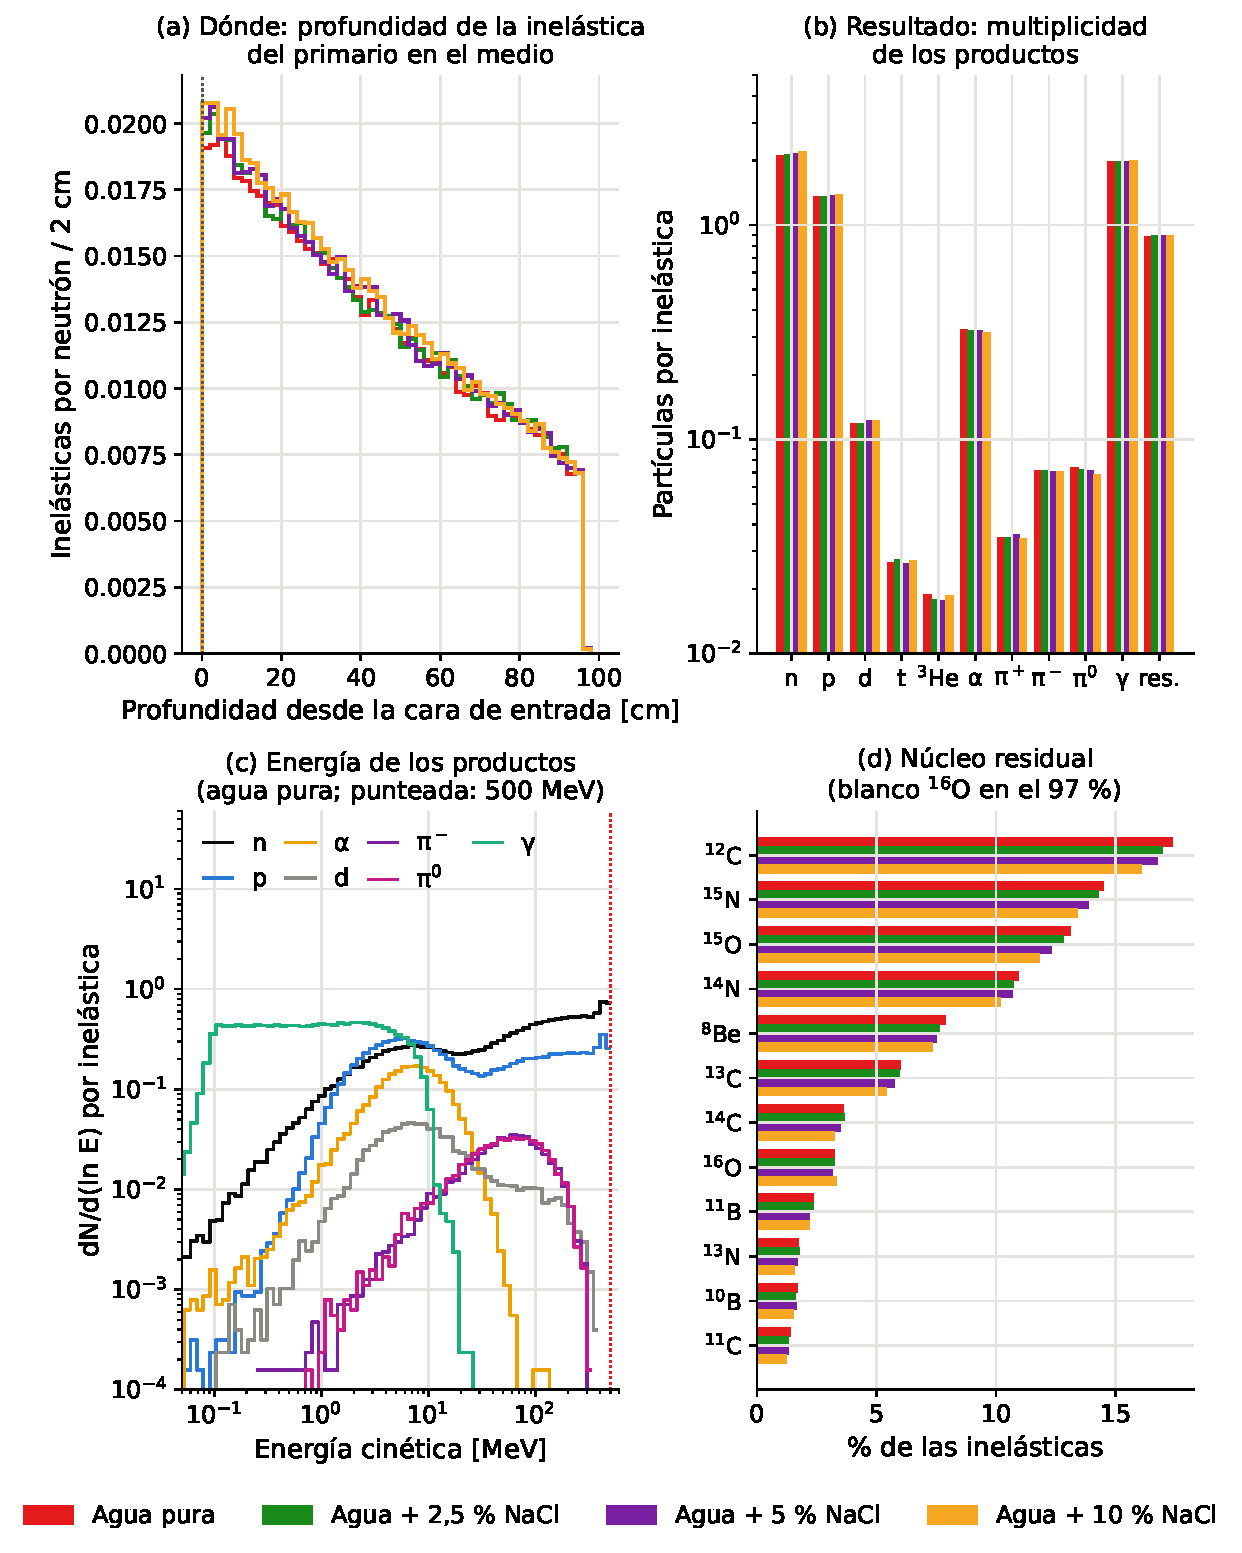
\includegraphics[width=\linewidth]{../figuras/fig20_inelasticas_primario.pdf}\caption{Interacciones inelásticas del neutrón primario de 500\,MeV: (a) profundidad a lo largo del haz en el medio; (b) multiplicidad media de los productos; (c) espectro de energía de los productos en agua pura; (d) núcleos residuales más frecuentes.}\label{fig:primario}\end{figure}
\subsection{¿Desaparece el primario? Consecuencias para la comparación con Sidelnik}\label{sec:primario_captura}
\paragraph{El primario casi nunca es el neutrón capturado.} De los primarios, el 61,7\,\% (agua pura), 62,6\,\% (2,5\,\% NaCl), 62,9\,\% (5\,\% NaCl) y 64,1\,\% (10\,\% NaCl) desaparece en una inelástica y el 37,4\,\% (agua pura), 36,6\,\% (2,5\,\% NaCl), 36,3\,\% (5\,\% NaCl) y 35,1\,\% (10\,\% NaCl) sale del tanque;
solo el 0,88\,\% (agua pura), 0,81\,\% (2,5\,\% NaCl), 0,78\,\% (5\,\% NaCl) y 0,76\,\% (10\,\% NaCl) se captura como la misma traza, después de frenarse únicamente por dispersiones elásticas.
En cambio, en el 97,0\,\% (agua pura), 97,3\,\% (2,5\,\% NaCl), 97,3\,\% (5\,\% NaCl) y 97,6\,\% (10\,\% NaCl) de los eventos con captura el primario tuvo antes una inelástica: los neutrones capturados son los secundarios, sobre todo los de evaporación, que se moderan en el agua;
por cada primario hay 2,44 (agua pura), 2,51 (2,5\,\% NaCl), 2,58 (5\,\% NaCl) y 2,73 (10\,\% NaCl) neutrones secundarios. Los eventos con captura tienen en promedio 1,95 (agua pura), 2,00 (2,5\,\% NaCl), 2,04 (5\,\% NaCl) y 2,12 (10\,\% NaCl) capturas.
Las diferencias entre medios son pequeñas (menos de 1,5 puntos porcentuales): con más sal el primario sufre algo más de inelásticas y escapa menos, hay algo más de neutrones secundarios y aumenta el número de capturas por evento, en parte porque el cloro captura neutrones que en agua pura escaparían del tanque.
Este comportamiento no es propio de MEIGA: es el de cualquier simulación con Geant4, incluida la de Sidelnik, porque los modelos de cascada intranuclear terminan la traza incidente y crean trazas nuevas para todos los productos.
Físicamente, además, los neutrones son indistinguibles: después de la inelástica no tiene sentido preguntar si se capturó ``el primario''.
\paragraph{Por eso nuestros resultados no contradicen a Sidelnik.} El 0,88\,\% mide la numeración de las trazas, no la física, y no es comparable con el 25,18\,\% del artículo.
La magnitud comparable es el número de capturas en el agua dividido por todos los neutrones del evento (primario + secundarios):
\begin{table}[H]\centering\small\begin{adjustbox}{max width=\linewidth}\begin{tabular}{lcccc}\toprule
 & Agua pura & 2,5\,\% NaCl & 5\,\% NaCl & 10\,\% NaCl \\\midrule
Primario capturado (misma traza) & 0,88\,\% & 0,81\,\% & 0,78\,\% & 0,76\,\% \\
Neutrones incidentes con $\geq 1$ captura en el agua & 42,4\,\% & 43,3\,\% & 44,3\,\% & 45,9\,\% \\
\textbf{Capturas / neutrones del evento (MEIGA)} & \textbf{24,08\,\%} & \textbf{24,59\,\%} & \textbf{25,19\,\%} & \textbf{26,08\,\%} \\
\textit{Sidelnik: probabilidad de captura} & \textit{25,18\,\%} & \textit{26,73\,\%} & \textit{27,65\,\%} & \textit{29,26\,\%} \\
Aumento relativo con NaCl (MEIGA) & -- & +2,1\,\% & +4,6\,\% & +8,3\,\% \\
\textit{Aumento relativo con NaCl (Sidelnik)} & -- & \textit{+6,2\,\%} & \textit{+9,8\,\%} & \textit{+16,2\,\%} \\
\bottomrule\end{tabular}\end{adjustbox}\caption{Tres formas de medir la captura. Solo la tercera es comparable con la Tabla~2 de Sidelnik.}\label{tab:defs_captura}\end{table}
En agua pura MEIGA queda 1,1 puntos por debajo del artículo (un 5\,\% relativo), una diferencia razonable entre dos simulaciones con versiones y modelos hadrónicos distintos
(Bertini produce más piones y más gammas de desexcitación nuclear, Secs.~\ref{sec:fig6} y \ref{sec:interp_fig5}).
La diferencia que sí debe discutirse es el efecto de la sal: la fracción aumenta un 2,1\,\% (2,5\,\%), 4,6\,\% (5\,\%), 8,3\,\% (10\,\%) en MEIGA (con 2,5\,\%, significativo a $\approx$\,6\,$\sigma$) frente al 6,2\,\%, 9,8\,\%, 16,2\,\% del artículo: la tendencia es la misma, pero unas dos veces más débil.
No es un error de nuestros datos: todos los medios usan la misma física y la misma geometría, y el tiempo de captura con NaCl sigue el valor teórico de las secciones eficaces térmicas (Sec.~\ref{sec:nacl25}; con 2,5\,\% NaCl, 140\,µs frente a 147\,µs).
Puede deberse a diferencias en las secciones eficaces del Cl o en la moderación entre las dos simulaciones, o a la normalización de Sidelnik, que el artículo no detalla.
\aviso{Recomendación para la tesis: reportar dos magnitudes y dejar el 0,88\,\% solo como nota metodológica:
(i) capturas por neutrón del evento, comparable con Sidelnik (24,1\,\% (agua pura), 24,6\,\% (2,5\,\% NaCl), 25,2\,\% (5\,\% NaCl) y 26,1\,\% (10\,\% NaCl)), y
(ii) fracción de neutrones incidentes que producen al menos una captura, que es la relevante para la eficiencia del detector (42,4\,\% (agua pura), 43,3\,\% (2,5\,\% NaCl), 44,3\,\% (5\,\% NaCl) y 45,9\,\% (10\,\% NaCl)).}
\subsection{Dispersiones elásticas: reconstrucción de los vértices}\label{sec:elasticas}
Las dispersiones elásticas (\texttt{hadElastic}) son las que moderan los neutrones antes de la captura. Se reconstruyeron todos los vértices elásticos de todos los neutrones
(\texttt{elasticas\_vertices.py}): 15\,573\,769 en agua pura (104 por neutrón incidente), 12\,519\,457 con 2,5\,\% NaCl (83 por neutrón incidente), 10\,732\,779 con 5\,\% NaCl (72 por neutrón incidente) y 8\,834\,631 con 10\,\% NaCl (59 por neutrón incidente).
Con sal hay menos vértices porque el Cl captura antes a los neutrones térmicos: la fracción de vértices por debajo de 1\,eV es del 74\,\%, 69\,\%, 65\,\% y 59\,\% (agua pura, 2,5\,\% NaCl, 5\,\% NaCl, 10\,\% NaCl, respectivamente).
La cinemática (masas reconstruidas, decrementos $\xi$ y conservación) coincide en todos los medios dentro de 0,002, por lo que las cifras que siguen son las del agua pura. Cada vértice es $n(E_{\rm in},\hat d_{\rm in}) + (A,Z) \to n(E_{\rm out},\hat d_{\rm out}) + (A,Z)_{\rm retroceso}$:
el neutrón entrante y el saliente se toman de \texttt{pasos-neutrones.tsv} (el vértice es el extremo del paso \texttt{hadElastic} y la dirección de salida, la del paso siguiente)
y el núcleo de retroceso, de \texttt{pasos-particulas.tsv} (partícula creada por \texttt{hadElastic}), enlazado por evento, traza madre y posición.
\paragraph{Con quién: el blanco reconstruido solo con el neutrón.} Con la transferencia de impulso $\vec q = \vec p_{\rm in} - \vec p_{\rm out}$ y la de energía $T = E_{\rm in} - E_{\rm out}$, la masa del blanco es $M = (q^2 - T^2)/(2T)$, sin usar el retroceso.
Por encima de 20\,MeV la mediana es 938,27\,MeV para el H (masa del protón: 938,27) y 14\,895,1\,MeV para el O (masa nuclear del $^{16}$O: 14\,895,1);
por debajo de 20\,MeV resulta 938,78 y 14\,899,1\,MeV, las masas \emph{atómicas} del $^1$H y del $^{16}$O (núcleo + electrones):
el modelo de alta precisión (\texttt{G4NeutronHP}, $<20$\,MeV) usa masas atómicas y el de alta energía, masas nucleares. Donde hay retroceso registrado, el blanco cinemático coincide con la partícula de retroceso en el 100,00\,\% de los vértices.
La composición por energía (Fig.~\ref{fig:elasticas}a) sigue las secciones eficaces: el H domina por debajo de 1\,MeV (85,6\,\% de las colisiones entre 1\,keV y 1\,MeV), el O gana peso por encima (44,8\,\% sobre 20\,MeV),
y con sal el Na y el Cl son el blanco en solo el 0,6\,\% (2,5\,\%), 1,0\,\% (5\,\%), 1,7\,\% (10\,\%) de las colisiones: la sal cambia la captura, no la moderación.
\paragraph{Energía y ángulo.} Para el H la fracción de energía perdida es uniforme entre 0 y 1 y para el $^{16}$O, uniforme entre 0 y 0,223 (Fig.~\ref{fig:elasticas}c), lo que corresponde a una dispersión isótropa en el centro de masas.
El decremento logarítmico medio $\xi = \langle\ln(E/E')\rangle$ medido es 1,000 para el H (teoría: 1) y 0,118 para el O (teoría: 0,121) entre 1\,keV y 1\,MeV.
Por encima de unos MeV la dispersión en el O se vuelve hacia adelante (difracción) y $\xi_O$ cae a 0,011 sobre 20\,MeV (Fig.~\ref{fig:elasticas}d,e): el neutrón de 500\,MeV apenas se frena en el O y se modera casi solo en el H.
\paragraph{Neutrones térmicos.} El 74\,\% de los vértices ocurre por debajo de 1\,eV, donde los neutrones difunden hasta capturarse. Allí el blanco no está en reposo (modelo de gas libre; esta corrida no usa $S(\alpha,\beta)$):
el 44\,\% de las colisiones aumenta la energía del neutrón y la reconstrucción con el blanco en reposo no es válida. Geant4 no registra el núcleo de retroceso por debajo de $\approx$\,1\,keV.
\paragraph{Leyes de conservación.} En cada vértice con retroceso la energía se conserva dentro de una parte en $10^3$ en el 99,998\,\% de los casos (el residuo de $\sim$\,$5\times10^{-4}$ proviene de la convención de masas atómicas)
y el impulso, dentro del 1\,\% en el 96,7\,\% (mediana $1{,}2\times10^{-4}$; el resto tiene la dirección del retroceso mal definida por un primer paso muy corto; Fig.~\ref{fig:elasticas}f).
La carga, el número bariónico y el leptónico se conservan exactamente: el estado inicial y el final son el mismo neutrón y el mismo núcleo ($A$ y $Z$ iguales, sin leptones),
y no aparecen núcleos de retroceso distintos de los del medio ($p$, $^{16,17,18}$O, $^{23}$Na, $^{35,37}$Cl) salvo en el Tyvek ($^{12}$C), en el acero ($^{56}$Fe, $^{52}$Cr), en el aire ($^{14}$N) y algunos deuterones del $^2$H natural del agua.
\begin{table}[H]\centering\small\begin{adjustbox}{max width=\linewidth}\begin{tabular}{lcccc}\toprule
Energía del neutrón & Vértices (agua pura) & Blanco H / O & $\xi_H$ & $\xi_O$ \\\midrule
1 eV--1 keV & 1\,002\,307 & 88,2\,\% / 5,5\,\% & 1,017 & 0,131 \\
1 keV--1 MeV & 1\,083\,824 & 85,6\,\% / 14,2\,\% & 1,000 & 0,118 \\
1--20 MeV & 413\,486 & 70,7\,\% / 28,4\,\% & 1,007 & 0,094 \\
$>$\,20 MeV & 194\,087 & 33,6\,\% / 44,8\,\% & 1,106 & 0,011 \\
\midrule Teoría (dispersión isótropa en el CM) &  &  & 1,000 & 0,121 \\
\bottomrule\end{tabular}\end{adjustbox}
\caption{Vértices elásticos por intervalo de energía, blanco reconstruido por cinemática y decremento logarítmico medio. Por debajo de 1\,eV (11\,466\,643 vértices) el blanco térmico no está en reposo y no se reconstruye.}\label{tab:elasticas}\end{table}
\begin{figure}[H]\centering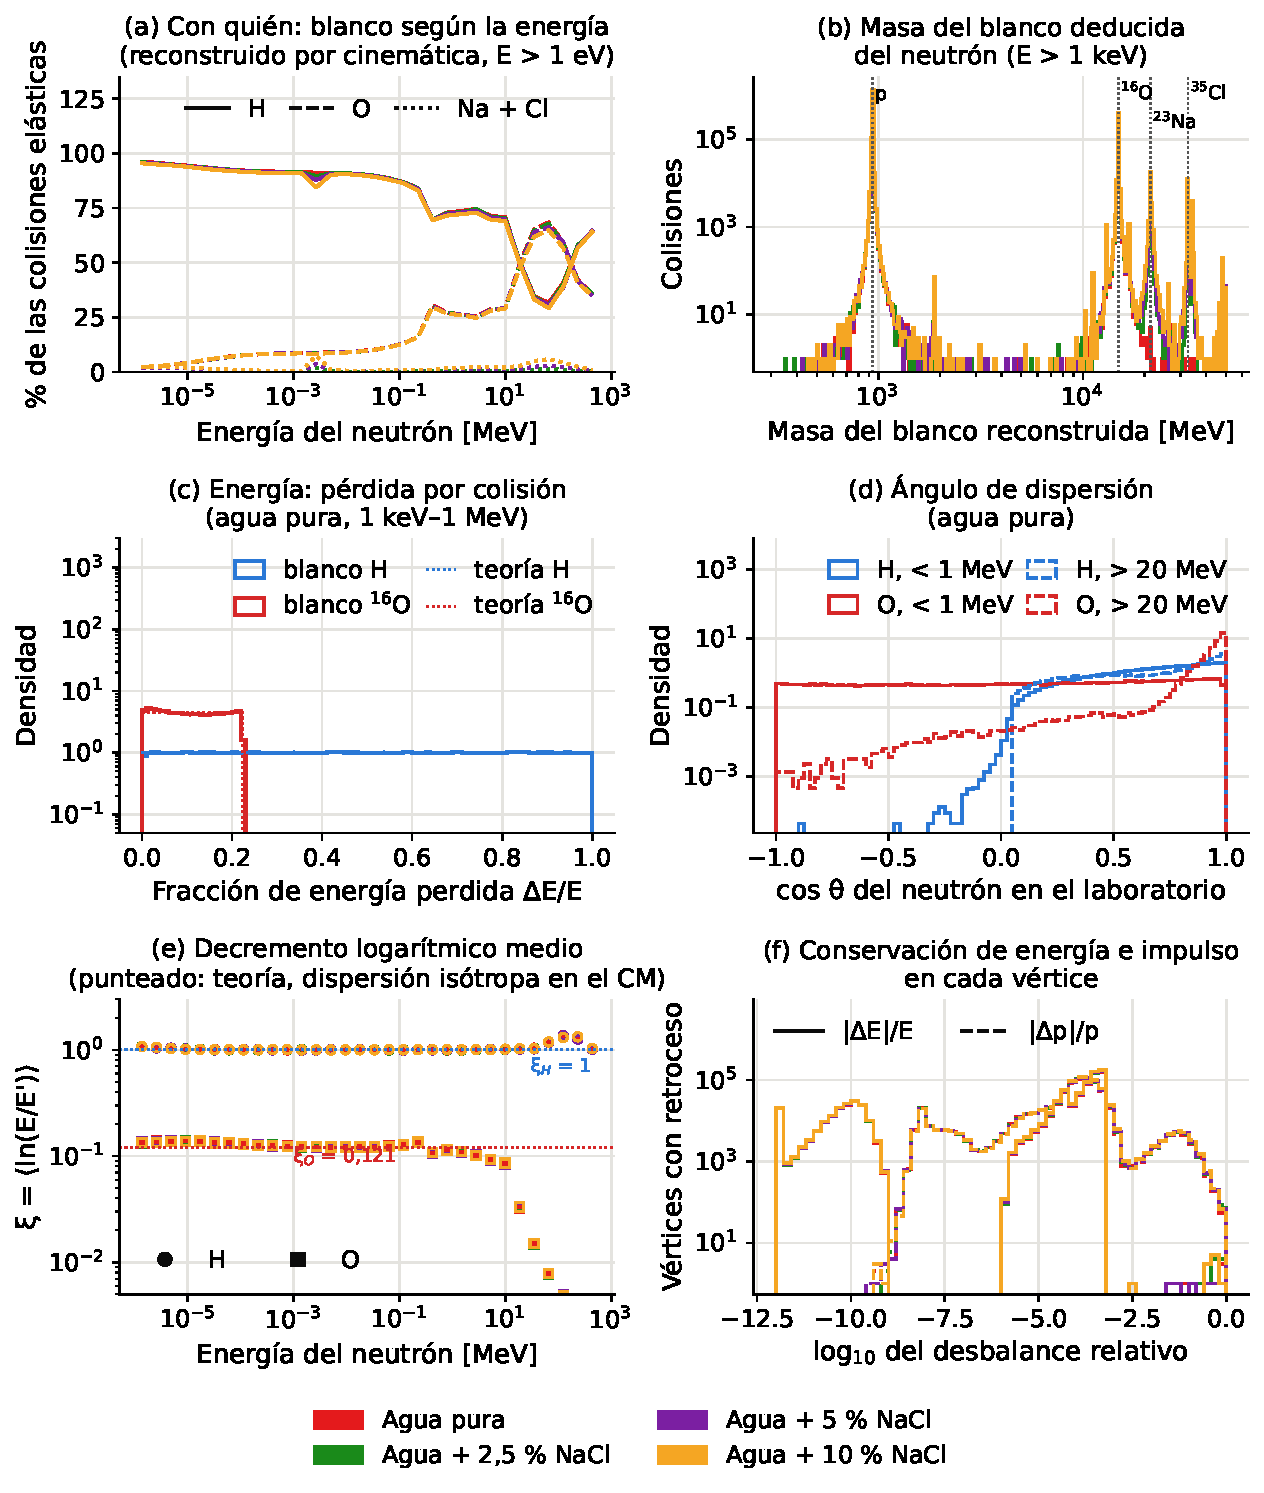
\includegraphics[width=\linewidth]{../figuras/fig21_elasticas.pdf}\caption{Reconstrucción de los vértices de dispersión elástica: (a) blanco según la energía del neutrón; (b) masa del blanco deducida solo de la cinemática del neutrón; (c) fracción de energía perdida por colisión en H y $^{16}$O frente a la teoría; (d) ángulo de dispersión en el laboratorio; (e) decremento logarítmico medio $\xi$; (f) balance de energía e impulso en cada vértice.}\label{fig:elasticas}\end{figure}
\paragraph{Esquema de la cinemática.} La Fig.~\ref{fig:esquema_cin} explica gráficamente estos resultados: con el H (masa casi igual a la del neutrón) neutrón y protón salen perpendiculares y el neutrón nunca retrocede; con el $^{16}$O el neutrón puede rebotar pero conserva al menos el 78\,\% de su energía.
El diagrama de velocidades muestra el porqué: la velocidad final es $\vec V_{CM} + \vec u\,'$, con $\vec u\,'$ isótropa sobre un círculo de radio $u' = Av/(A+1)$; para el H el círculo pasa por el origen y para el O lo encierra.
Por encima de 20\,MeV solo el O dispersa hacia adelante (difracción); el H sigue cercano a la dispersión isótropa en el CM.
\begin{figure}[H]\centering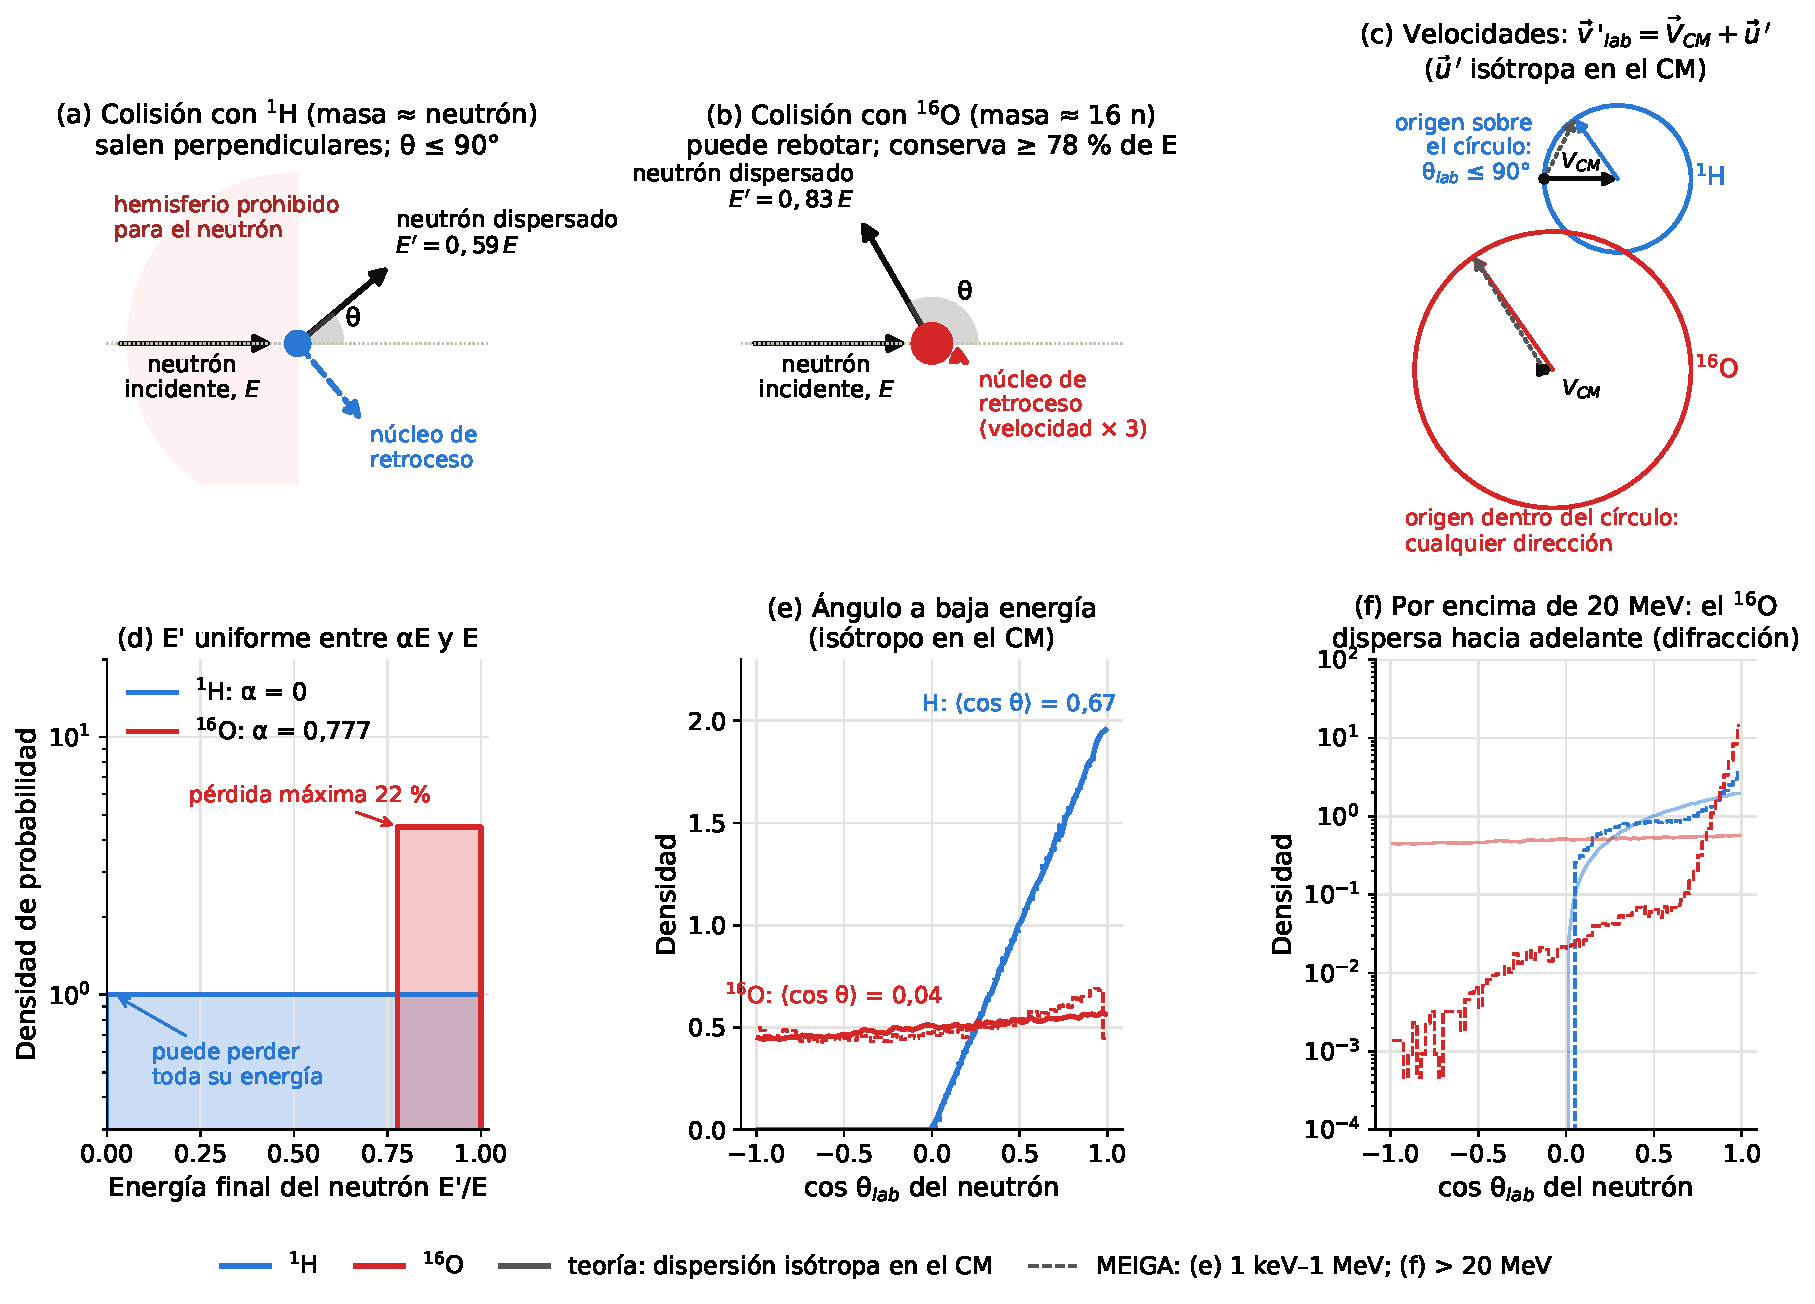
\includegraphics[width=\linewidth]{../figuras/fig23_esquema_cinematica_elastica.pdf}\caption{Cinemática de la dispersión elástica: (a) colisión con $^1$H; (b) colisión con $^{16}$O (velocidad del retroceso $\times$3); (c) diagrama de velocidades; (d) energía final uniforme entre $\alpha E$ y $E$; (e) $\cos\theta_{\rm lab}$ entre 1\,keV y 1\,MeV, teoría frente a MEIGA (agua pura); (f) por encima de 20\,MeV.}\label{fig:esquema_cin}\end{figure}
\subsection{Ecuaciones, energías y porcentajes de todos los procesos}\label{sec:procesos_resumen}
Las tablas completas de reacciones de cada medio (ecuación, valor $Q$, energía típica del neutrón, porcentaje y gammas emitidos) están en el Apéndice~\ref{sec:procesos}.
Explican de dónde vienen los gammas, y por tanto los electrones y la luz Cherenkov: la dispersión elástica en H modera ($\xi = 1$), la captura en H y en $^{35}$Cl produce los gammas de captura,
y las inelásticas en $^{16}$O (canales (n,n$'$), (n,n$\alpha$), (n,np), (n,2n) y los de fragmentación a más de 20\,MeV) producen el fondo de desexcitación nuclear y los emisores $\beta^+$.
\paragraph{De dónde salen los gammas de 4--7\,MeV.} Cada inelástica emite en promedio 0,24 gammas entre 4 y 7\,MeV.
Según el núcleo que los emite: $^{16}$O 29\,\% (dispersión inelástica $^{16}$O(n,n$'$)), $^{12}$C 21\,\% ($^{16}$O(n,n$\alpha$)$^{12}$C y canales de fragmentación),
$^{15}$N 16\,\% ($^{16}$O(n,np)$^{15}$N), $^{14}$N 10\,\% y $^{15}$O 9\,\% ($^{16}$O(n,2n)$^{15}$O).
Pero solo el 12\,\% son líneas discretas: 6130\,keV del $^{16}$O (7,0\,\%), 4439\,keV del $^{12}$C (2,4\,\%),
6917\,keV del $^{16}$O (1,9\,\%) y, con menos del 0,3\,\% cada una, las del $^{15}$N (5269, 5298, 6324\,keV), $^{15}$O (5183, 5241, 6176) y $^{14}$N (5106).
La razón es el modelo: el 22\,\% de estos gammas viene de neutrones de menos de 20\,MeV, tratados con los datos evaluados de \texttt{G4NeutronHP}, y entre ellos el 48\,\% son líneas;
el resto viene de reacciones de más de 20\,MeV (cascada de Bertini), cuya desexcitación es estadística y produce un continuo (solo el 2\,\% son líneas).
Por eso el fondo de 4--7\,MeV de la Sec.~\ref{sec:interp_fig5} es sobre todo un continuo de desexcitación con unas pocas líneas encima, y su intensidad depende del modelo de cascada.
\subsection{Captura de neutrones (Tabla 2 de Sidelnik)}
\begin{table}[H]\centering\small\begin{adjustbox}{max width=\linewidth}\begin{tabular}{lcccc}\toprule
 & Agua pura & 2,5\,\% NaCl & 5\,\% NaCl & 10\,\% NaCl \\\midrule
Capturas en el agua por neutrón primario & 0,829 & 0,864 & 0,903 & 0,972 \\
Neutrones en el evento por primario (primario + cascada) & 3,44 & 3,51 & 3,58 & 3,73 \\
\textbf{Capturas en el agua / todos los neutrones} & \textbf{24,08\,\%} & \textbf{24,59\,\%} & \textbf{25,19\,\%} & \textbf{26,08\,\%} \\
Neutrones con $\geq 1$ captura en el agua & 42,43\,\% & 43,30\,\% & 44,27\,\% & 45,95\,\% \\
Primario de 500\,MeV capturado (la misma traza) & 0,88\,\% & 0,81\,\% & 0,78\,\% & 0,76\,\% \\
\textit{Sidelnik: probabilidad de captura} & \textit{25,18\,\%} & \textit{26,73\,\%} & \textit{27,65\,\%} & \textit{29,26\,\%} \\
Capturas fuera del agua (acero, Tyvek, aire) & 184 & 135 & 131 & 83 \\
Capturas en H & 99,94\,\% & 63,53\,\% & 47,53\,\% & 30,95\,\% \\
Capturas en $^{35}$Cl & 0,00\,\% & 35,75\,\% & 51,47\,\% & 67,66\,\% \\
Tiempo de captura $\tau$ [µs] & 192 & 140 & 109 & 75 \\
Energía de captura, mediana [meV] & 30,5 & 30,6 & 31,0 & 31,7 \\
\bottomrule\end{tabular}\end{adjustbox}\caption{Captura de neutrones en el volumen activo.}\end{table}
\aviso{Qué mide el 25,18\,\% de Sidelnik. El artículo lo describe como ``la fracción de capturas de neutrones dentro del volumen activo'' sin decir sobre qué total.
Las tres definiciones posibles dan, en agua pura:
(i) capturas por neutrón primario: 0,829 (un mismo primario de 500\,MeV produce en promedio 3,4 neutrones y varios se capturan);
(ii) captura de la traza primaria: 0,88\,\%, porque en Geant4 el neutrón de 500\,MeV desaparece casi siempre en su primera interacción inelástica y los neutrones que salen de ella son trazas nuevas; no es comparable con el artículo;
(iii) capturas divididas por todos los neutrones del evento (primario + cascada): 24,08\,\%,
que coincide con el 25,18\,\% de Sidelnik dentro de 1\,punto. Esta es la interpretación adoptada: de cada cuatro neutrones que existen en el tanque, uno termina capturado en el agua; los demás escapan o se pierden en interacciones inelásticas. Con 2,5\,\% NaCl la fracción sube a 24,59\,\% (+2,1\,\% relativo; Sidelnik: 26,73\,\%, +6,2\,\%).}

\subsection{Distancia de máxima absorción (Fig. 2 de Sidelnik)}
\begin{table}[H]\centering\small\begin{adjustbox}{max width=\linewidth}\begin{tabular}{lcccc}\toprule
 & Agua pura & 2,5\,\% NaCl & 5\,\% NaCl & 10\,\% NaCl \\\midrule
Borde de entrada $\to$ captura, a lo largo del haz: máximo [cm] & 46,5 & 45,3 & 36,1 & 47,8 \\
Vértice del neutrón capturado $\to$ captura: máximo [cm] & 11,1 & 10,0 & 9,8 & 9,6 \\
Inelástica del primario $\to$ captura: máximo [cm] & 12,7 & 11,3 & 11,2 & 10,4 \\
\textit{Sidelnik: distancia de máxima absorción [cm]} & \textit{8,4} & \textit{8,0} & \textit{7,7} & \textit{7,3} \\
\bottomrule\end{tabular}\end{adjustbox}\caption{Distancia de máxima absorción con tres definiciones (máximo del histograma suavizado de 0,5\,cm).}\end{table}
Medida a lo largo del haz desde la cara de entrada, la distribución de capturas de MEIGA es una joroba ancha con máximo cerca del centro del tanque
(46,5\,cm): el primario de 500\,MeV hace su primera inelástica en promedio a 40\,cm de profundidad,
y los neutrones de la cascada se capturan en todo el volumen. La forma de la Fig.~2 de Sidelnik (máximo cercano y cola larga hasta $\sim$96\,cm) sí aparece
si la distancia se mide desde el punto donde nace el neutrón capturado (máximo a 11,1\,cm) o desde la inelástica del primario
(12,7\,cm). Esto sugiere que la ``distancia desde el borde'' de Sidelnik describe en realidad la escala de moderación.
La curva de agua pura de Sidelnik se digitalizó de la figura del artículo; solo se recuperan los 43 puntos rojos visibles (en la cola los tapan los de las otras curvas).
\begin{figure}[H]\centering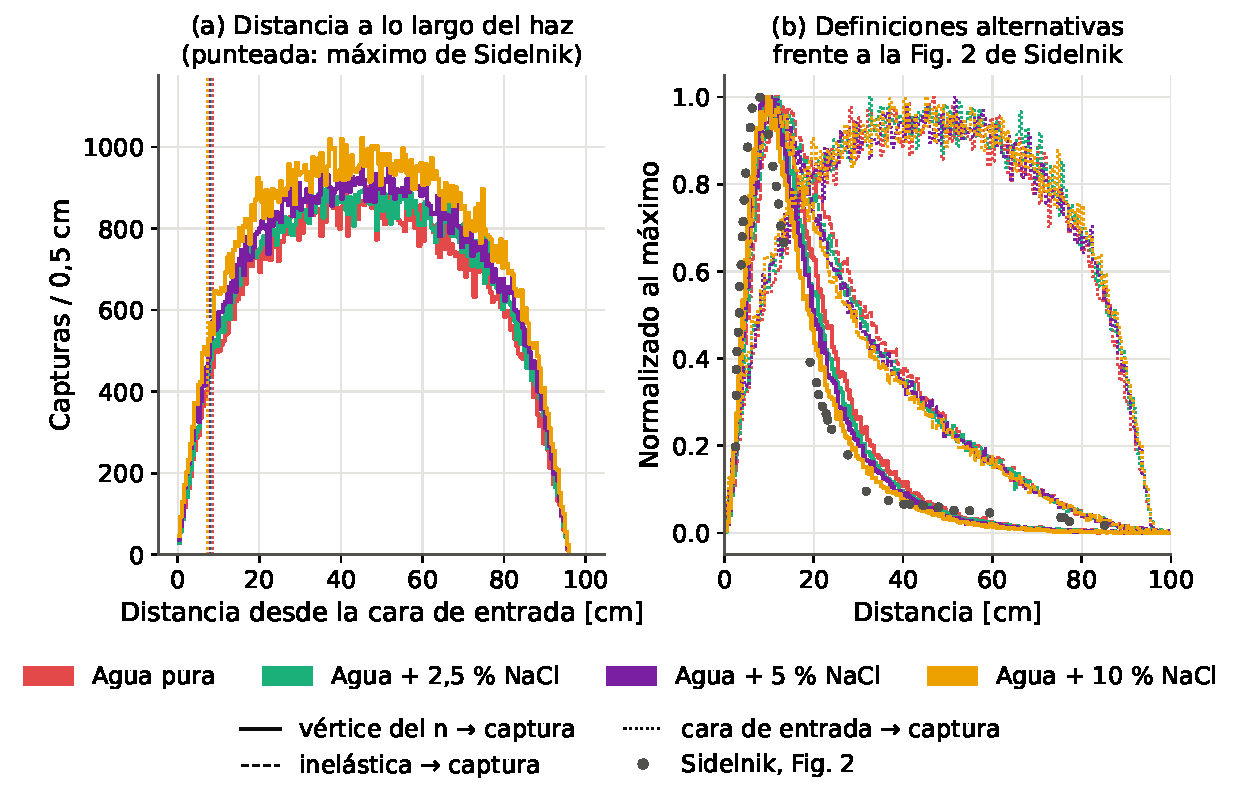
\includegraphics[width=\linewidth]{../figuras/fig01_distancia_captura.pdf}\caption{Izquierda: capturas en función de la distancia a lo largo del haz desde la cara de entrada. Derecha: tres definiciones de distancia, normalizadas, frente a la curva de agua pura digitalizada de Sidelnik (puntos).}\end{figure}
\subsection{Efecto del NaCl en la captura}\label{sec:nacl25}
Las corridas con NaCl usan exactamente el mismo esquema que la de agua pura (física sin $S(\alpha,\beta)$, Tyvek y PMT iguales; 150\,000 neutrones cada una); solo cambia el medio
(composición de la Ec.~3.12 y densidad e índice de refracción de la Tabla~3.6). Por eso las diferencias entre medios se deben al NaCl, y su comparación con las tendencias de Sidelnik
es válida aunque el modelo óptico del Tyvek se revise después. Entre paréntesis, el cambio relativo respecto al agua pura.
\begin{table}[H]\centering\small\begin{adjustbox}{max width=\linewidth}\begin{tabular}{lcccc}\toprule
 & Agua pura & 2,5\,\% & 5\,\% & 10\,\% \\\midrule
Capturas / neutrones del evento (MEIGA) & 24,08\,\% & 24,59\,\% (+2,1\,\%) & 25,19\,\% (+4,6\,\%) & 26,08\,\% (+8,3\,\%) \\
\textit{Sidelnik: probabilidad de captura} & 25,18\,\% & 26,73\,\% (+6,2\,\%) & 27,65\,\% (+9,8\,\%) & 29,26\,\% (+16,2\,\%) \\
Neutrones incidentes con $\geq 1$ captura & 42,43\,\% & 43,30\,\% (+2,0\,\%) & 44,27\,\% (+4,3\,\%) & 45,95\,\% (+8,3\,\%) \\
Capturas por neutrón incidente & 0,829 & 0,864 (+4,3\,\%) & 0,903 (+8,9\,\%) & 0,972 (+17,3\,\%) \\
Capturas en H & 99,9\,\% & 63,5\,\% & 47,5\,\% & 31,0\,\% \\
Capturas en $^{35}$Cl (MEIGA) & 0,0\,\% & 35,8\,\% & 51,5\,\% & 67,7\,\% \\
\quad teoría (secciones eficaces térmicas) & 0,0\,\% & 28,0\,\% & 44,2\,\% & 62,2\,\% \\
Capturas en $^{23}$Na / $^{37}$Cl & 0,0\,\% / 0,0\,\% & 0,6\,\% / 0,1\,\% & 0,8\,\% / 0,2\,\% & 1,1\,\% / 0,2\,\% \\
Tiempo de captura $\tau$ [µs] (MEIGA) & 192 & 140 (-27,0\,\%) & 109 (-43,2\,\%) & 75 (-61,0\,\%) \\
\quad teoría [µs] & 205 & 147 (-28,0\,\%) & 114 (-44,2\,\%) & 78 (-62,1\,\%) \\
Vértice $\to$ captura, máximo [cm] & 11,1 & 10,0 (-10,2\,\%) & 9,8 (-11,7\,\%) & 9,6 (-13,6\,\%) \\
\textit{Sidelnik: distancia de máxima absorción [cm]} & 8,4 & 8,0 (-4,8\,\%) & 7,7 (-8,3\,\%) & 7,3 (-13,1\,\%) \\
Energía de gammas de captura por neutrón [MeV] & 1,85 & 4,39 (+136,9\,\%) & 5,71 (+208,0\,\%) & 7,40 (+299,2\,\%) \\
\bottomrule\end{tabular}\end{adjustbox}\caption{Captura en los distintos medios (MEIGA, 150\,000 neutrones de 500\,MeV por medio) frente a las tendencias de Sidelnik.}\label{tab:nacl}\end{table}
Las tendencias tienen el signo del artículo y son monótonas con la concentración: aumenta la fracción de captura y se acorta la distancia de captura. El aumento de la fracción de captura es menor que en el artículo
(2,5\,\%: +2,1\,\% frente a +6,2\,\%, 5\,\%: +4,6\,\% frente a +9,8\,\%, 10\,\%: +8,3\,\% frente a +16,2\,\%),
mientras que el tiempo de captura sigue la predicción de las secciones eficaces térmicas (2,5\,\%: 140 frente a 147\,µs, 5\,\%: 109 frente a 114\,µs, 10\,\%: 75 frente a 78\,µs).
La fracción de capturas en $^{35}$Cl es mayor que la que dan esas secciones eficaces (2,5\,\%: 35,8\,\% frente a 28,0\,\%, 5\,\%: 51,5\,\% frente a 44,2\,\%, 10\,\%: 67,7\,\% frente a 62,2\,\%),
un exceso ya observado en las campañas anteriores con G4NDL\,4.6.
\subsection{Espectros de captura por núcleo (Fig. 4.1 de la tesis)}\label{sec:captura_nucleo}
La Fig.~\ref{fig:captnucleo} reproduce la Fig.~4.1 de la tesis con estas corridas: gammas emitidos en cada captura, enlazados con el núcleo que capturó el neutrón.
La línea del H se ajusta a una gaussiana con $\mu = 2224{,}37301$\,keV y $\sigma \approx 0{,}013$\,keV, los mismos valores de la Fig.~4.1 (2224,37301\,keV; 0,01285\,keV). El gamma de Geant4 tiene $E_\gamma \approx S_n(^2{\rm H}) = 2224{,}57$\,keV menos 0,2\,keV, mientras que el valor medido es 2223,25\,keV ($S_n$ menos el retroceso del deuterón, 1,32\,keV):
la línea de MEIGA está 1,1\,keV por encima de la real y, como el deuterón recibe además su energía de retroceso (Sec.~\ref{sec:deut}), cada captura en H libera $\approx$\,1,1\,keV más que $S_n$. El efecto es irrelevante para la luz, pero conviene citarlo junto a la Fig.~4.1(b).
\begin{table}[H]\centering\small\begin{adjustbox}{max width=\linewidth}\begin{tabular}{rcc}\toprule
Línea del $^{35}$Cl(n,$\gamma$) [keV] & MEIGA [por 100 capturas] & Referencia ENSDF [por 100 capturas] \\\midrule
1\,164,9 & 25,8 & 26,8 \\
8\,579,8 & 24,4 & -- (no existe) \\
517,1 & 23,1 & 22,8 \\
6\,110,9 & 19,1 & 19,8 \\
1\,951,1 & 18,2 & 19,1 \\
788,4 & 14,9 & 16,3 \\
1\,959,4 & 11,7 & 12,3 \\
7\,413,9 & 10,2 & 9,9 \\
786,3 & 9,9 & 10,3 \\
7\,790,3 & 8,1 & 8,0 \\
\bottomrule\end{tabular}\end{adjustbox}\caption{Intensidad de las líneas principales de la captura en $^{35}$Cl (46\,355 capturas). Referencia: evaluación ENSDF (Nica et al.~2012), intensidades PGAA/OIEA por 100 capturas.}\end{table}
Las líneas de la cascada (517, 788, 1165, 1951, 6111, 7414\,keV) tienen, por captura, intensidades muy cercanas a las de referencia; la excepción es un gamma de 8579,8\,keV, presente en el 24\,\% de las capturas, que no es la transición real al fundamental (8578,70\,keV, 2,7\,\%, bien reproducida) sino un gamma único con toda la energía $S_n$ (Sec.~\ref{sec:esquemas}).
En esas capturas el gamma sale solo (y conserva la energía), mientras que en las demás los gammas de la cascada se sortean de forma independiente: su suma vale en promedio 10,6\,MeV y menos del 1\,\% suma $Q$.
Es el comportamiento del modelo de captura de alta precisión de Geant4 (\texttt{G4NeutronHP}), que toma los gammas de las tablas de producción de fotones de la evaluación (ENDF/G4NDL) sin imponer la conservación de la energía en cada captura;
Geant4 permite en cambio usar \texttt{G4PhotonEvaporation}, que genera cascadas que sí la conservan (variable de entorno \texttt{G4NEUTRONHP\_USE\_ONLY\_PHOTONEVAPORATION}). En la Fig.~4.1(c) de la tesis, obtenida con otra simulación, la línea de 8,58\,MeV es pequeña.
Los paneles (a) y (d) tienen poca estadística (77 capturas en $^{16}$O en agua pura y 141 en $^{37}$Cl con 2,5\,\% NaCl).
\begin{figure}[H]\centering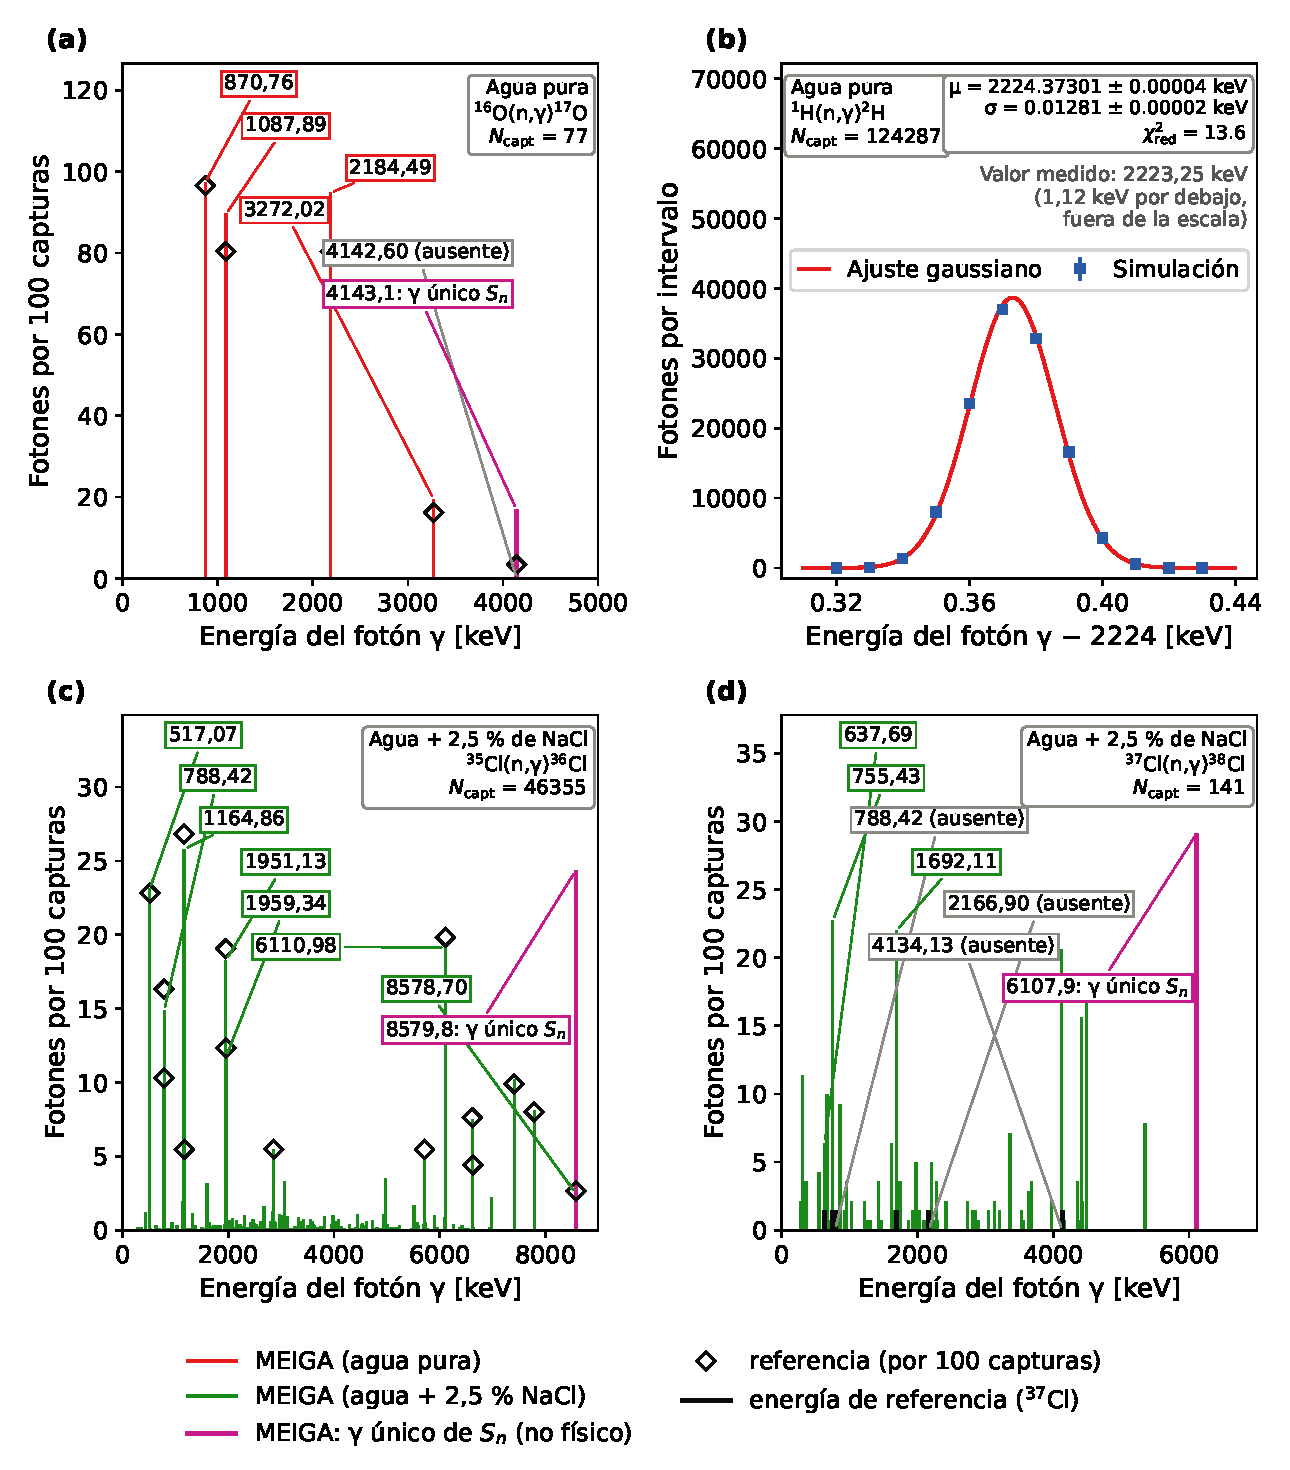
\includegraphics[width=\linewidth]{../figuras/fig15_espectros_captura_nucleo.pdf}\caption{Espectros gamma de la captura de neutrones por núcleo (formato de la Fig.~4.1 de la tesis): (a) $^{16}$O(n,$\gamma$)$^{17}$O en agua pura; (b) $^{1}$H(n,$\gamma$)$^{2}$H con ajuste gaussiano; (c) $^{35}$Cl(n,$\gamma$)$^{36}$Cl y (d) $^{37}$Cl(n,$\gamma$)$^{38}$Cl en agua + 2,5\,\% NaCl. Intensidad en fotones por 100 capturas; los rombos son los valores de referencia (Firestone y Révay 2016 para $^{16}$O; ENSDF, Nica et al.~2012, para $^{35}$Cl) y las marcas negras en (d) las energías de la Tabla~4.2. Las etiquetas dan, en keV, la energía de referencia de cada línea (las de la Tabla~4.2 unificada, Sec.~\ref{sec:tabla42}); en magenta, el gamma único de $S_n$ que emite Geant4.}\label{fig:captnucleo}\end{figure}
\subsection{Esquemas de niveles: $^{35}$Cl(n,$\gamma$)$^{36}$Cl y $^{16}$O(n,$\gamma$)$^{17}$O}\label{sec:esquemas}
La Fig.~\ref{fig:Cl36} muestra el esquema de niveles de $^{36}$Cl con las quince transiciones más intensas de la captura de neutrones térmicos en $^{35}$Cl,
con los datos de la evaluación ENSDF (N.~Nica, J.~Cameron y B.~Singh, Nucl.\ Data Sheets 113, 1 (2012); intensidades de la base PGAA del OIEA, convertidas
a fotones por 100 capturas con $\sigma_{Z\gamma} = 33{,}22$\,b). Entre corchetes se dan las intensidades de MEIGA en las 214\,748 capturas en $^{35}$Cl.
La Fig.~\ref{fig:O17} muestra lo mismo para $^{17}$O (Fig.~4.2 de la tesis; Firestone y Révay 2016), con las 190 capturas en $^{16}$O de todas las corridas.
\paragraph{Lo que reproduce MEIGA.} En el $^{35}$Cl, 13 de las 15 transiciones coinciden con la evaluación dentro de pocos puntos porcentuales, incluidas las primarias
(6110,98\,keV: 19,4\,\% frente a 19,8\,\%; 7414,09\,keV: 10,0\,\% frente a 9,9\,\%)
y la transición directa al fundamental (8578,70\,keV: 2,6\,\% frente a 2,7\,\%). Las excepciones son la línea de 1170,94\,keV (0,5\,\% frente a 5,5\,\%),
casi ausente en los datos de MEIGA, y la de 788,42\,keV, algo baja. En el $^{16}$O, las transiciones de la cascada coinciden dentro del error estadístico.
\paragraph{Lo que no reproduce: un gamma único con toda la energía de separación.} Además de las transiciones reales, Geant4 emite en el 24,3\,\% de las capturas en $^{35}$Cl
un único gamma de 8579,8\,keV, igual a $S_n$ sin la corrección por retroceso del núcleo (la transición real al fundamental tiene 8578,70\,keV). En el $^{16}$O ocurre lo mismo:
el 21,6 $\pm$ 3,4\,\% de las capturas emite un único gamma de 4143,09\,keV ($S_n$ de $^{17}$O), mientras que la transición real de 4142,60\,keV no aparece
(0 casos, frente a 3,36\,\% esperado). La misma fracción en dos núcleos distintos ($\approx$\,24\,\%) indica que el origen está en el código de captura de Geant4 y no en los datos nucleares.
En el resto de las capturas los gammas de la cascada se sortean de forma independiente: su suma promedia 10,1\,MeV en el Cl (el promedio incluye las capturas con el gamma único).
Por eso las intensidades por captura de las líneas coinciden con la evaluación mientras la energía depositada por captura no se conserva (Sec.~\ref{sec:nacl25}).
\begin{landscape}\begin{figure}[p]\centering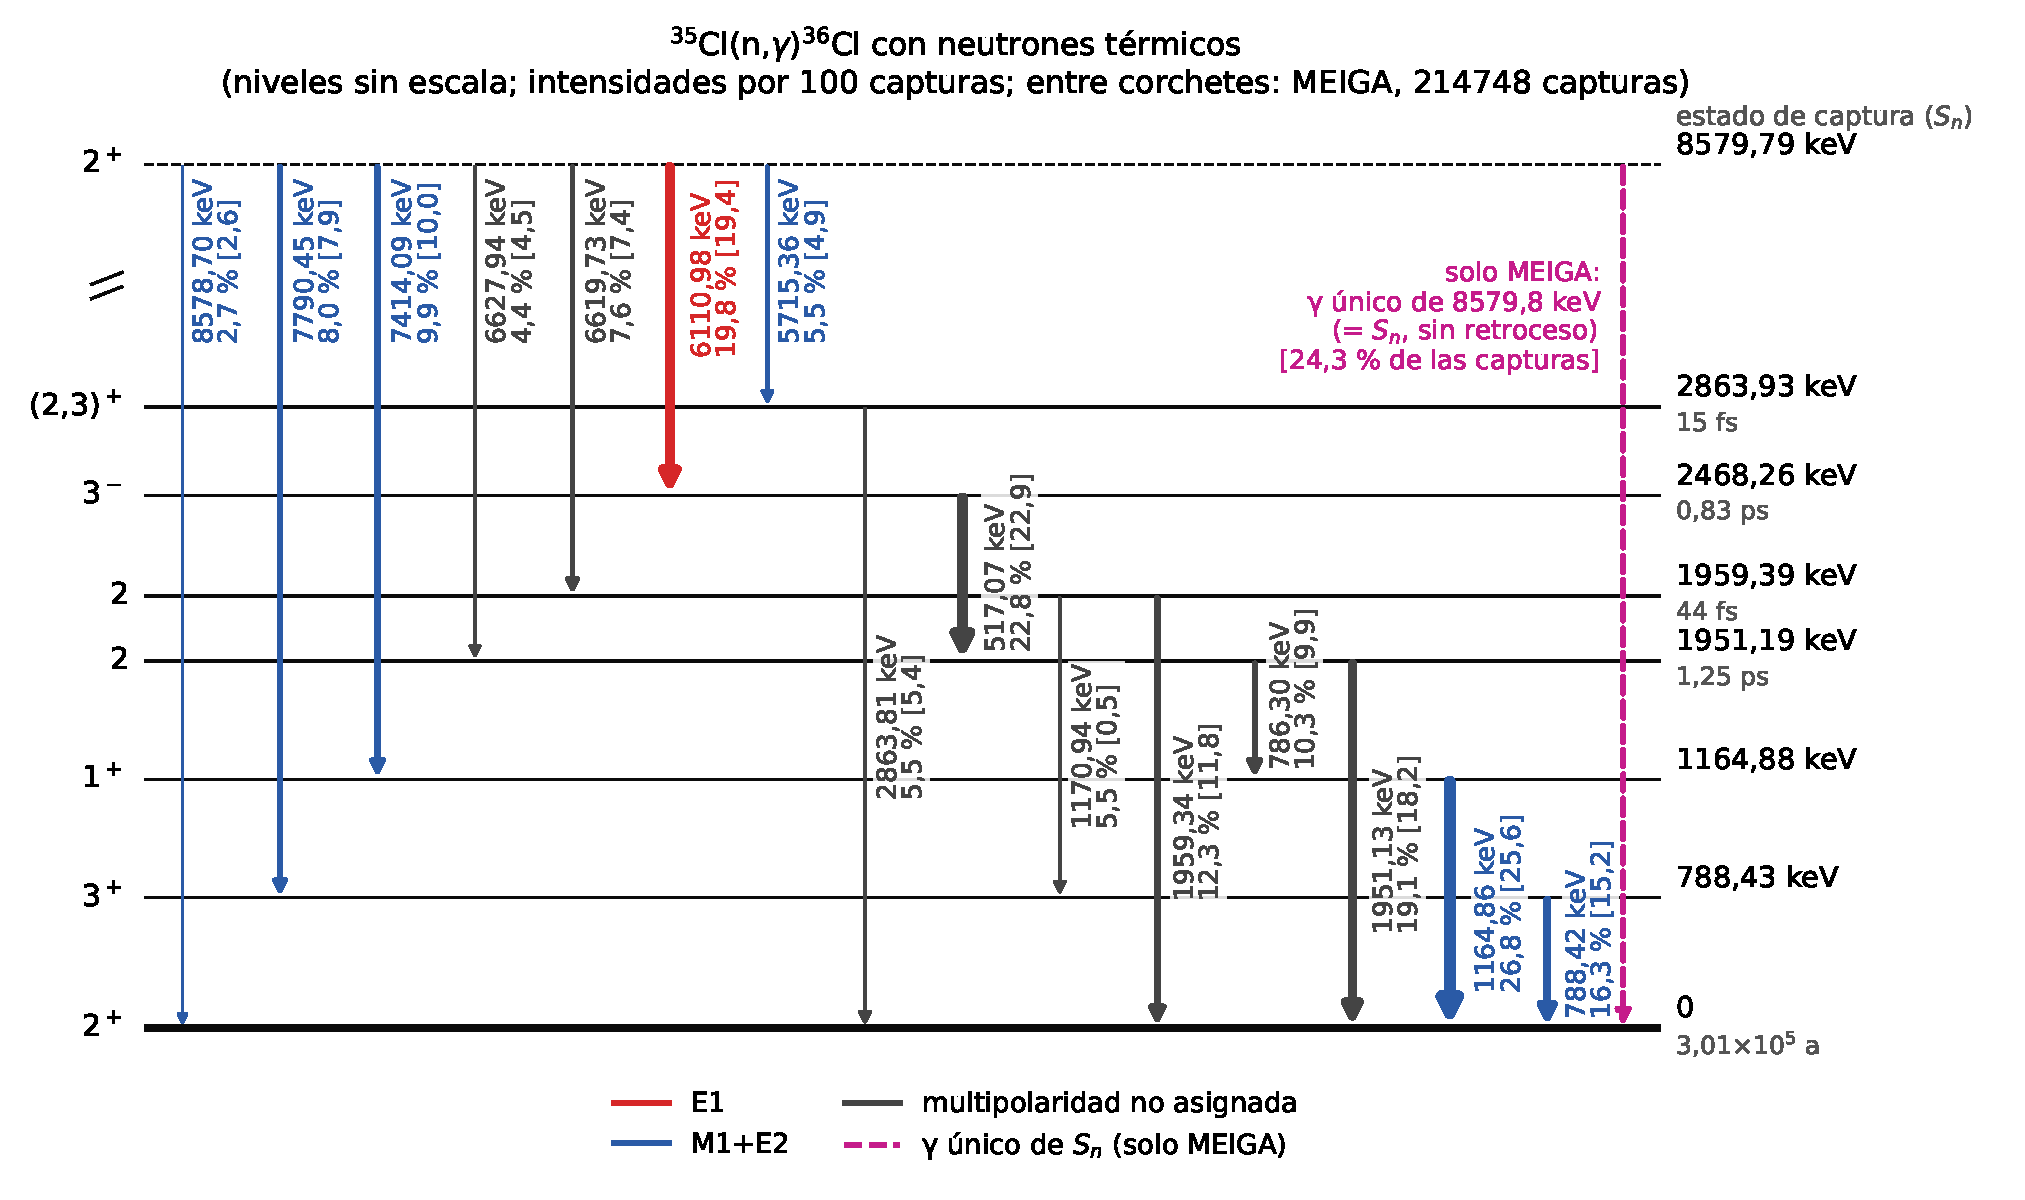
\includegraphics[width=\linewidth,height=0.86\textheight,keepaspectratio]{../figuras/fig19b_esquema_niveles_Cl36_MEIGA.pdf}\caption{Esquema de niveles de $^{36}$Cl y transiciones $\gamma$ más intensas de la captura $^{35}$Cl(n,$\gamma$) con neutrones térmicos (ENSDF, Nica et al.\ 2012; niveles sin escala). Intensidades por 100 capturas; entre corchetes, MEIGA. En magenta, el gamma único de energía $S_n$ que emite Geant4. La versión sin MEIGA está en \texttt{figuras/fig19\_esquema\_niveles\_Cl36}.}\label{fig:Cl36}\end{figure}\end{landscape}
\begin{figure}[H]\centering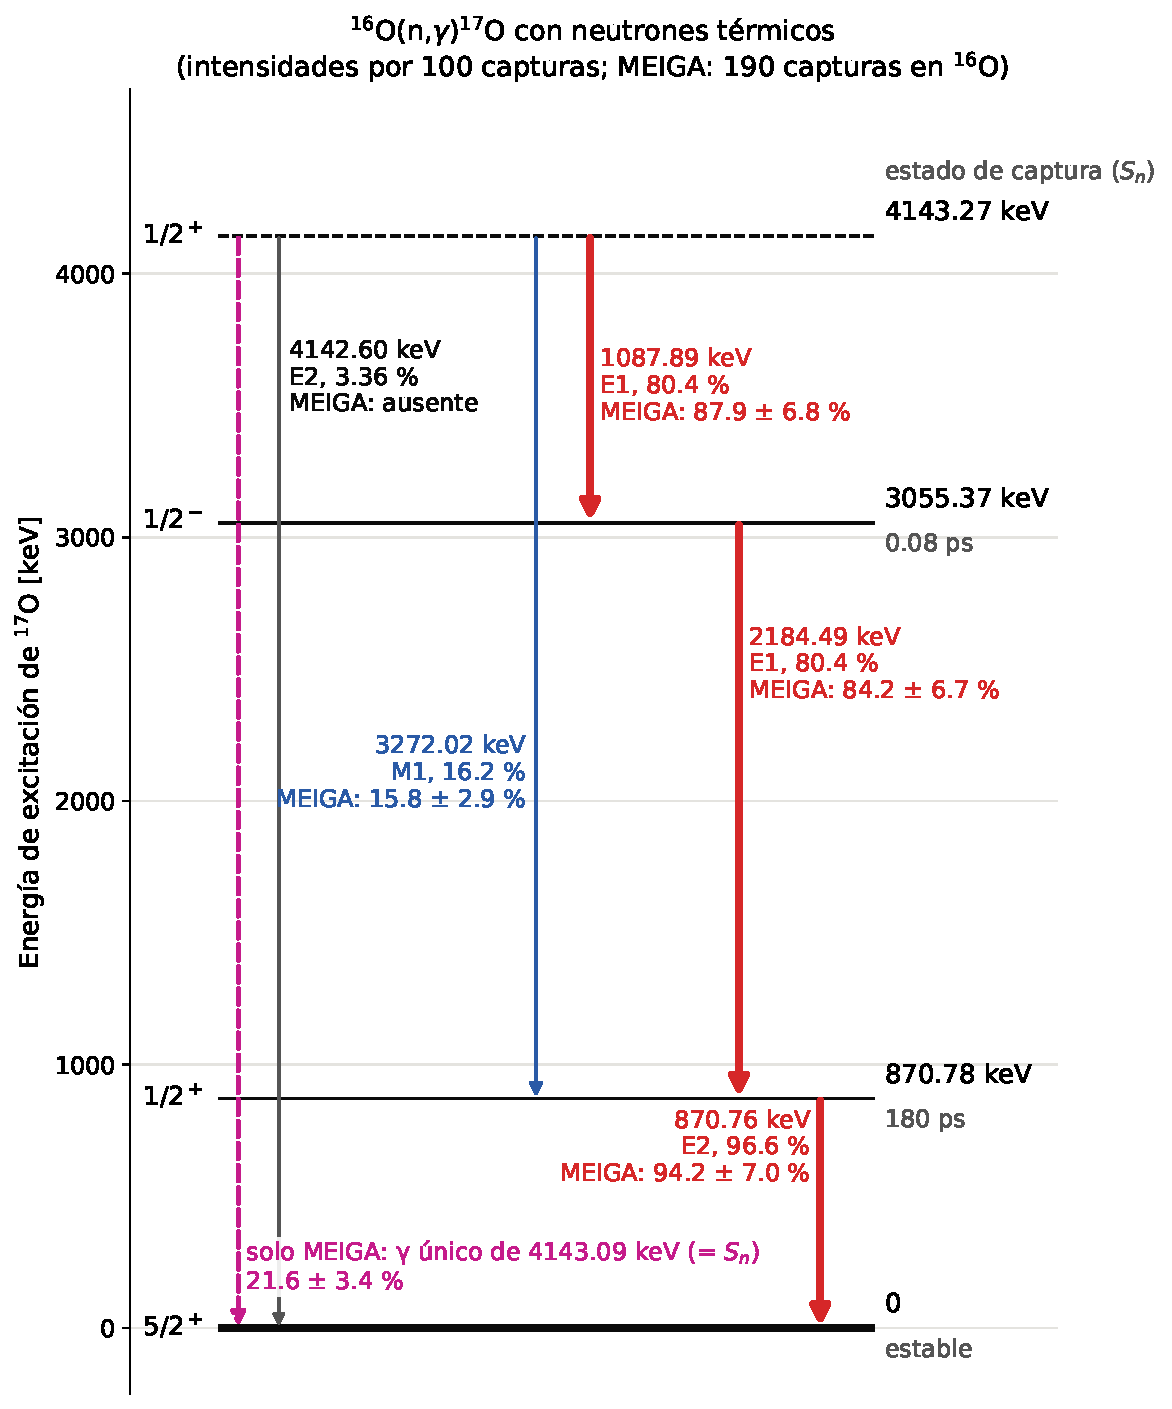
\includegraphics[width=0.85\linewidth]{../figuras/fig18b_esquema_niveles_O17_MEIGA.pdf}\caption{Esquema de niveles y transiciones $\gamma$ de la captura $^{16}$O(n,$\gamma$)$^{17}$O con neutrones térmicos (Firestone y Révay, Phys.\ Rev.\ C 93, 044311, 2016; CapGam/NNDC) e intensidades por 100 capturas en MEIGA; en magenta, el gamma único de energía $S_n$. La réplica de la Fig.~4.2 está en \texttt{figuras/fig18\_esquema\_niveles\_O17}.}\label{fig:O17}\end{figure}
\subsection{Parámetros nucleares y líneas de captura (Tabla 4.2 de la tesis)}\label{sec:tabla42}
La Tabla~\ref{tab:tabla42} reproduce la Tabla~4.2 de la tesis (abundancias, sección eficaz térmica de captura radiativa $\sigma_0$ y energías de las líneas $\gamma$, contrastadas con CapGam/NNDC;
para $^{16}$O, Firestone y Révay 2016). Las energías marcadas con $^\dagger$ se corrigieron para que coincidan con las de las figuras de este informe (ver la leyenda). La última columna da la misma transición en MEIGA (a menos de 0,4\,keV; para el H, la línea de Geant4 está 1,1\,keV por encima) y su intensidad por 100 capturas en ese isótopo.
\begin{table}[H]\centering\footnotesize
\begin{adjustbox}{max width=\linewidth}\begin{tabular}{cccrr}\toprule
\multicolumn{5}{c}{\textbf{Parámetros nucleares y líneas $\gamma$ de captura}}\\\midrule
\textbf{Isótopo} & \textbf{\shortstack{Abundancia\\isotópica (\%)}} & \textbf{$\sigma_0$ (mb)} & \textbf{$E_\gamma$ (keV)} & \textbf{\shortstack{MEIGA: $E_\gamma$ (keV)\\(por 100 capturas)}}\\\midrule
\rowcolor{gray!15}$^{1}$H & 99,99 & $332{,}60 \pm 0{,}70$ & 2\,223,25 & 2\,224,37 \;(100,0\,\%) \\
\midrule
$^{16}$O & 99,76 & $0{,}170 \pm 0{,}003$ & 870,76 & 870,80 \;(94,2\,\%) \\
 &  &  & 1\,087,89$^\dagger$ & 1\,088,00 \;(87,9\,\%) \\
 &  &  & 2\,184,49$^\dagger$ & 2\,184,20 \;(84,7\,\%) \\
 &  &  & 3\,272,02$^\dagger$ & 3\,272,20 \;(15,8\,\%) \\
 &  &  & 4\,142,60$^\dagger$ & -- \\
 & \multicolumn{3}{r}{\textcolor{magenta!70!black}{$\gamma$ único de $S_n$ (solo MEIGA)}} & \textcolor{magenta!70!black}{4\,143,09 \;(21,6\,\%)} \\
\midrule
\rowcolor{gray!15}$^{35}$Cl & 75,78 & $43840 \pm 170$ & 517,07 & 517,08 \;(22,9\,\%) \\
\rowcolor{gray!15} &  &  & 788,42 & 788,43 \;(15,2\,\%) \\
\rowcolor{gray!15} &  &  & 1\,164,86 & 1\,164,87 \;(25,6\,\%) \\
\rowcolor{gray!15} &  &  & 1\,951,13$^\dagger$ & 1\,951,14 \;(18,2\,\%) \\
\rowcolor{gray!15} &  &  & 1\,959,34$^\dagger$ & 1\,959,36 \;(11,8\,\%) \\
\rowcolor{gray!15} &  &  & 6\,110,98$^\dagger$ & 6\,110,85 \;(19,4\,\%) \\
\rowcolor{gray!15} &  &  & 8\,578,70$^\dagger$ & 8\,578,59 \;(2,6\,\%) \\
\rowcolor{gray!15} & \multicolumn{3}{r}{\textcolor{magenta!70!black}{$\gamma$ único de $S_n$ (solo MEIGA)}} & \textcolor{magenta!70!black}{8\,579,81 \;(24,3\,\%)} \\
\midrule
$^{23}$Na & 100 & $527 \pm 7$ & 472,20 & 472,26 \;(0,6\,\%) \\
 & \multicolumn{3}{r}{\textcolor{magenta!70!black}{$\gamma$ único de $S_n$ (solo MEIGA)}} & \textcolor{magenta!70!black}{6\,959,44 \;(11,4\,\%)} \\
\midrule
\rowcolor{gray!15}$^{37}$Cl & 24,22 & $553 \pm 17$ & 637,69 & 637,50 \;(11,5\,\%) \\
\rowcolor{gray!15} &  &  & 755,43 & 755,47 \;(26,0\,\%) \\
\rowcolor{gray!15} &  &  & 788,42 & -- \\
\rowcolor{gray!15} &  &  & 1\,692,11 & 1\,692,15 \;(19,9\,\%) \\
\rowcolor{gray!15} &  &  & 2\,166,90 & -- \\
\rowcolor{gray!15} &  &  & 4\,134,13 & -- \\
\rowcolor{gray!15} & \multicolumn{3}{r}{\textcolor{magenta!70!black}{$\gamma$ único de $S_n$ (solo MEIGA)}} & \textcolor{magenta!70!black}{6\,107,88 \;(28,1\,\%)} \\
\bottomrule\end{tabular}\end{adjustbox}
\caption{Parámetros nucleares de los principales isótopos del volumen activo y energías de las líneas $\gamma$ de captura de neutrones térmicos (Tabla~4.2 de la tesis), y la línea correspondiente en MEIGA
(capturas en el agua de las corridas de todos los medios: $^{1}$H 316\,177, $^{16}$O 190, $^{35}$Cl 214\,748, $^{23}$Na 3\,483, $^{37}$Cl 707). $\sigma_0$ es la sección eficaz total de captura radiativa térmica del isótopo, no la de producción de cada línea.
$^\dagger$Energías unificadas con las figuras de este informe (Firestone y Révay 2016 para $^{16}$O, como en la Fig.~4.2; ENSDF, Nica et al.~2012, para $^{35}$Cl, como en el esquema de $^{36}$Cl); entre paréntesis, el valor de la Tabla~4.2 original: $^{16}$O 1\,087,89\,keV (1\,087,86); $^{16}$O 2\,184,49\,keV (2\,184,44); $^{16}$O 3\,272,02\,keV (3\,272,15); $^{16}$O 4\,142,60\,keV (4\,142,73); $^{35}$Cl 1\,951,13\,keV (1\,959,13); $^{35}$Cl 1\,959,34\,keV (añadida); $^{35}$Cl 6\,110,98\,keV (6\,110,84); $^{35}$Cl 8\,578,70\,keV (8\,578,21). En magenta, el gamma único con toda la energía de separación que emite Geant4 (no existe en la naturaleza).}\label{tab:tabla42}\end{table}
{\small\textit{Nota de la tesis:} para $^{16}$O, Firestone y Révay reportan $\sigma_0 = 0{,}170\pm0{,}003$\,mb (2016, Sec.~II.B.1); la transición de $870{,}76\pm0{,}08$\,keV tiene una probabilidad absoluta de emisión $P_\gamma = 96{,}6\pm0{,}5$\,\%
(Tabla~III), mientras que su sección eficaz individual de producción es $\sigma_\gamma = 0{,}164\pm0{,}003$\,mb (Sec.~II.A, Tabla~I). Por tanto $\sigma_0$ y $\sigma_\gamma$ son magnitudes diferentes.}

\paragraph{Observaciones para la tesis.}
\begin{itemize}
\item \textbf{$^{1}$H:} la línea medida es 2223,25\,keV; MEIGA la emite a 2224,37\,keV (1,1\,keV más; Sec.~\ref{sec:captura_nucleo}).
\item \textbf{$^{16}$O:} en la Tabla~4.2 original las energías (1087,86; 2184,44; 3272,15; 4142,73\,keV) no coincidían con las de la Fig.~4.2 (1087,89; 2184,49; 3272,02; 4142,60\,keV), aunque ambas citan a Firestone y Révay (2016); aquí se usan las de la figura.
La transición real de 4142,60\,keV no aparece en MEIGA; en su lugar, el 21,6\,\% de las capturas emite el gamma único de 4143,09\,keV ($S_n$).
\item \textbf{$^{35}$Cl:} el valor 1959,13\,keV de la tabla original mezclaba dos líneas reales, 1951,13\,keV (19,1 por 100 capturas) y 1959,34\,keV (12,3), que ahora figuran por separado; la transición al fundamental pasa de 8578,21 a 8578,70\,keV (ENSDF)
y la de 6110,84 a 6110,98\,keV. Con estas energías MEIGA reproduce las siete líneas, incluida la del fundamental (2,4 frente a 2,7 por 100 capturas); aparte, el 24\,\% de las capturas emite el gamma único de 8579,81\,keV.
\item \textbf{$^{23}$Na:} MEIGA prácticamente no produce la línea de 472,20\,keV (0,6\,\%, frente a una línea dominante en la naturaleza): en el 11\,\% de las capturas emite el gamma único de 6959,4\,keV ($S_n$ de $^{24}$Na) y en el resto gammas de energías dispersas, sin líneas definidas.
\item \textbf{$^{37}$Cl:} también aquí el 28\,\% de las capturas emite el gamma único de $S_n$ (6107,9\,keV). Con 707 capturas aparecen las líneas de 637,5, 755,5 y 1692,2\,keV; las de 788,42, 2166,90 y 4134,13\,keV no aparecen.
\end{itemize}
\subsection{Las cascadas del $^{35}$Cl en Geant4 no conservan la energía}\label{sec:cascadas_cl}
La captura en $^{35}$Cl libera $Q=8{,}579$\,MeV, que en la naturaleza se reparte en una cascada de 3--4 gammas; la transición directa al estado fundamental (un solo gamma de 8,58\,MeV) ocurre en $\approx$\,3\,\% de las capturas.
En MEIGA (Geant4 10.7.p04, G4NDL\,4.6) las 46\,355 capturas en $^{35}$Cl emiten en promedio 2,80 gammas con una energía total media de 10,14\,MeV
(percentiles 5--95: 2,8--20,9\,MeV): solo el 26\,\% de las cascadas suma $Q$ (dentro del 1\,\%), el 43\,\% emite más energía y el 31\,\% menos,
y el 24\,\% de las capturas emite un único gamma de 8,58\,MeV. Esto explica el exceso de la línea de 8,58\,MeV. Las capturas en H, en cambio, emiten siempre un gamma de 2,224\,MeV.
\aviso{Consecuencia: en los medios con NaCl la luz de las capturas en Cl tiene, en promedio, un 18\,\% más de energía de la que corresponde, y con una dispersión que no es física.
Es un defecto del modelo de captura de Geant4/G4NDL, independiente del Tyvek; afecta a la escala de luz y de carga de los medios con NaCl y debe declararse en la tesis. Las intensidades de las líneas intermedias (1,165, 6,11, 7,41, 7,79\,MeV) sí coinciden con Sidelnik.}
\begin{figure}[H]\centering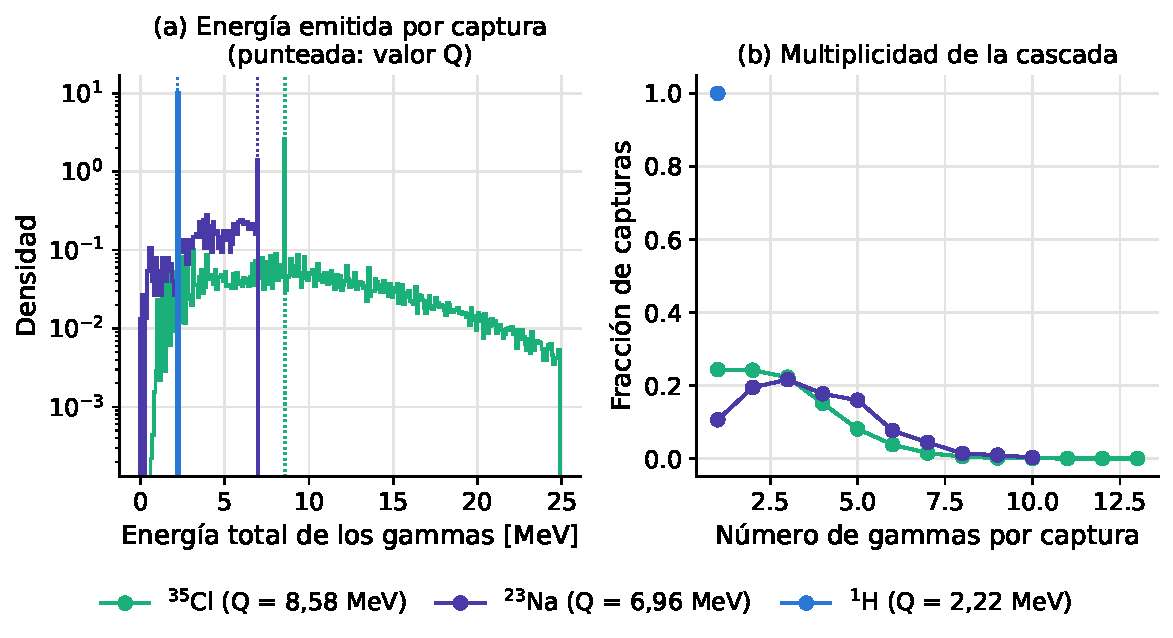
\includegraphics[width=\linewidth]{../figuras/fig12_cascadas_cloro_nacl25.pdf}\caption{Energía total emitida por captura y multiplicidad de la cascada en $^{35}$Cl, $^{23}$Na y $^{1}$H (agua + 2,5\,\% NaCl, MEIGA).}\end{figure}

\section{Comparación de los espectros de fotones gamma generados por captura de neutrones}
{\small\textit{Corresponde a la Sec.~4.1.1.3 de la tesis (Figs. 4.3 y 4.4).}}

\subsection{Gammas creados en el agua (Figs. 3 y 4 de Sidelnik)}
\begin{table}[H]\centering\small\begin{adjustbox}{max width=\linewidth}\begin{tabular}{lcccc}\toprule
 & Agua pura & 2,5\,\% NaCl & 5\,\% NaCl & 10\,\% NaCl \\\midrule
Gammas creados en el agua por neutrón & 5,98 & 7,03 & 7,68 & 8,65 \\
\quad de inelásticas de neutrones & 2,63 & 2,70 & 2,77 & 2,93 \\
\quad de captura & 0,83 & 1,43 & 1,76 & 2,19 \\
\quad bremsstrahlung / aniquilación & 1,23 / 0,67 & 1,42 / 0,76 & 1,56 / 0,82 & 1,74 / 0,90 \\
Energía gamma de captura por neutrón [MeV] & 1,855 & 4,393 & 5,713 & 7,404 \\
e$^\pm$ creados por gammas por neutrón & 44,1 & 51,4 & 55,8 & 62,2 \\
\quad Compton / fotoeléctrico & 37,1 / 6,80 & 41,4 / 9,57 & 43,6 / 11,74 & 46,3 / 15,25 \\
\quad fracción sobre umbral Cherenkov (0,264\,MeV) & 8,0\,\% & 8,3\,\% & 8,5\,\% & 8,7\,\% \\
\bottomrule\end{tabular}\end{adjustbox}\caption{Gammas y electrones creados dentro del agua.}\end{table}
\begin{figure}[H]\centering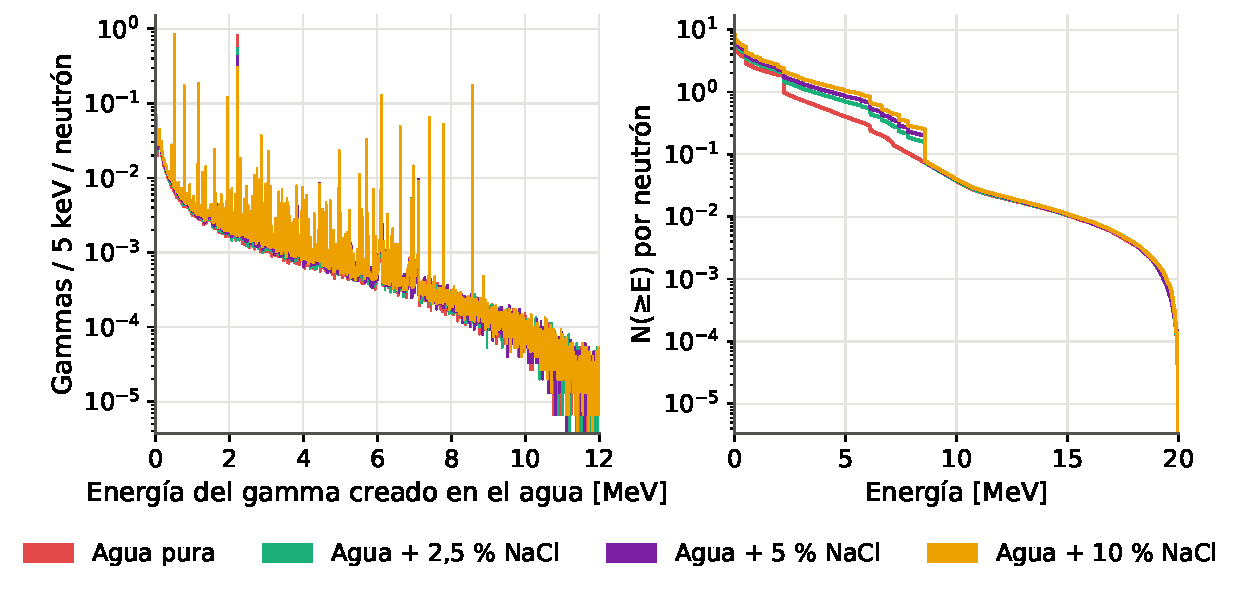
\includegraphics[width=\linewidth]{../figuras/fig02_espectro_gamma.pdf}\caption{Espectro de energía de los gammas creados en el agua (como la Fig.~3 de Sidelnik) y cuentas acumuladas de derecha a izquierda (como su Fig.~4).}\end{figure}
\paragraph{¿Por qué las curvas acumuladas con NaCl tienen una protuberancia entre 2,2 y 8,6\,MeV?}
$N(\geq E)$ cuenta, por neutrón, los gammas de energía mayor o igual que $E$: cada línea produce un escalón en su energía y los gammas comprendidos entre dos energías forman la meseta que las separa.
En agua pura casi todos los gammas de captura proceden del H y tienen 2,22\,MeV, de modo que por encima del escalón de 2,22\,MeV no queda ninguno.
Con NaCl, el $^{35}$Cl emite su cascada entre 2,3 y 8,58\,MeV: esos gammas forman una meseta adicional que termina en un escalón abrupto en 8,58\,MeV, la energía de separación del neutrón en el $^{36}$Cl, por encima de la cual no puede haber gammas de captura.
Por encima de 8,6\,MeV las curvas coinciden, porque allí solo quedan gammas de las inelásticas, del bremsstrahlung y de las desintegraciones de $\pi^0$ y muones, que no dependen de la sal (Tabla~\ref{tab:protuberancia}).
\begin{table}[H]\centering\small\begin{adjustbox}{max width=\linewidth}\begin{tabular}{lcccc}\toprule
Gammas creados en el agua por neutrón incidente & Agua pura & 2,5\,\% NaCl & 5\,\% NaCl & 10\,\% NaCl \\\midrule
$N(\geq 4\,$MeV$)$ total & 0,694 & 1,041 & 1,222 & 1,450 \\
\quad de captura (nCapture) & 0,000 & 0,332 & 0,498 & 0,705 \\
\quad de inelásticas de neutrones & 0,418 & 0,428 & 0,437 & 0,458 \\
Exceso sobre el agua pura en $N(\geq 4\,$MeV$)$ & -- & 0,346 & 0,528 & 0,756 \\
\quad fracción del exceso debida a la captura & -- & 96\,\% & 94\,\% & 93\,\% \\
Gammas de captura entre 2,3 y 8,7\,MeV por neutrón & 0,000 & 0,463 & 0,694 & 0,984 \\
\quad por captura en $^{35}$Cl & -- & 1,50 & 1,49 & 1,50 \\
Escalón de 8,58\,MeV (gamma único, por neutrón) & 0,000 & 0,083 & 0,126 & 0,176 \\
\quad fracción de las capturas en $^{35}$Cl & -- & 27\,\% & 27\,\% & 27\,\% \\
$N(\geq 8{,}7\,$MeV$)$ total & 0,216 & 0,216 & 0,219 & 0,217 \\
\bottomrule\end{tabular}\end{adjustbox}
\caption{Descomposición de las cuentas acumuladas $N(\geq E)$ de la figura anterior (derecha) por proceso creador (\texttt{gammas\_acumulados.py}).}\label{tab:protuberancia}\end{table}
La captura explica el 96\,\% (2,5\,\% NaCl) y el 94\,\% (5\,\% NaCl) y el 93\,\% (10\,\% NaCl) del exceso sobre el agua pura a 4\,MeV;
las inelásticas apenas cambian con la sal. Cada captura en $^{35}$Cl aporta unos 1,5 gammas entre 2,3 y 8,7\,MeV, y los escalones de la meseta son las líneas del $^{36}$Cl
(2,86, 5,72, 6,12, 6,62, 7,41 y 7,79\,MeV; Sec.~\ref{sec:cl_lineas}). El escalón mayor, en 8,57\,MeV, corresponde al 27\,\% de las capturas en $^{35}$Cl:
es el defecto de \texttt{G4NeutronHP} discutido en la Sec.~\ref{sec:cascadas_cl}, que en una cuarta parte de las capturas emite un único gamma con toda la energía de separación.
Con cascadas realistas el escalón de 8,58\,MeV sería mucho menor y la meseta tendría más gammas de menor energía.
Las caídas pequeñas cerca de 6--7\,MeV presentes también en el agua pura son las líneas de desexcitación del $^{16}$O (6,13, 6,92 y 7,12\,MeV) producidas por las inelásticas, iguales en todos los medios.
\subsubsection{Comparación con la Fig. 3 de Sidelnik}\label{sec:fig3}
\paragraph{Procedimiento.} Se histogramó la energía de creación de los 874\,916 gammas creados en el agua
(primer paso de cada gamma en \texttt{pasos-gamma.tsv}) con bines de 1\,keV, y se agruparon en bines de 2\,keV para el formato de la figura.
La Fig.~3 del artículo se digitalizó automáticamente por el color de los píxeles (\texttt{digitalizar\_fig3.py}); la curva roja de agua pura queda tapada en parte por las de NaCl,
por lo que su lectura es fiable en las líneas y en el continuo inferior, y aproximada por encima de 10\,MeV, donde hay pocas cuentas.
\paragraph{Normalización.} El eje de Sidelnik está en unidades arbitrarias: su línea de 2,223\,MeV tiene unas $4{,}2\times10^{5}$ cuentas, más que el número de neutrones
(150\,000) y unas diez veces más que las capturas que reporta (25\,\%). En MEIGA la línea tiene 124\,397 cuentas, una por captura en H;
contar todos los pasos de los gammas en vez de un gamma por entrada solo la sube a $1{,}8\times10^5$. Por eso la comparación se hace con magnitudes que no dependen de la normalización:
(i) cocientes entre alturas de líneas, que tampoco dependen del ancho de bin, y (ii) la forma del continuo con el pico de 2,223\,MeV igualado.
Con bines de 2\,keV el cociente pico/continuo de MEIGA entre 3 y 5\,MeV (1\,777--3\,659) coincide con el de Sidelnik (1\,946--3\,075), lo que sugiere que el artículo usó bines de ese orden.
\begin{figure}[H]\centering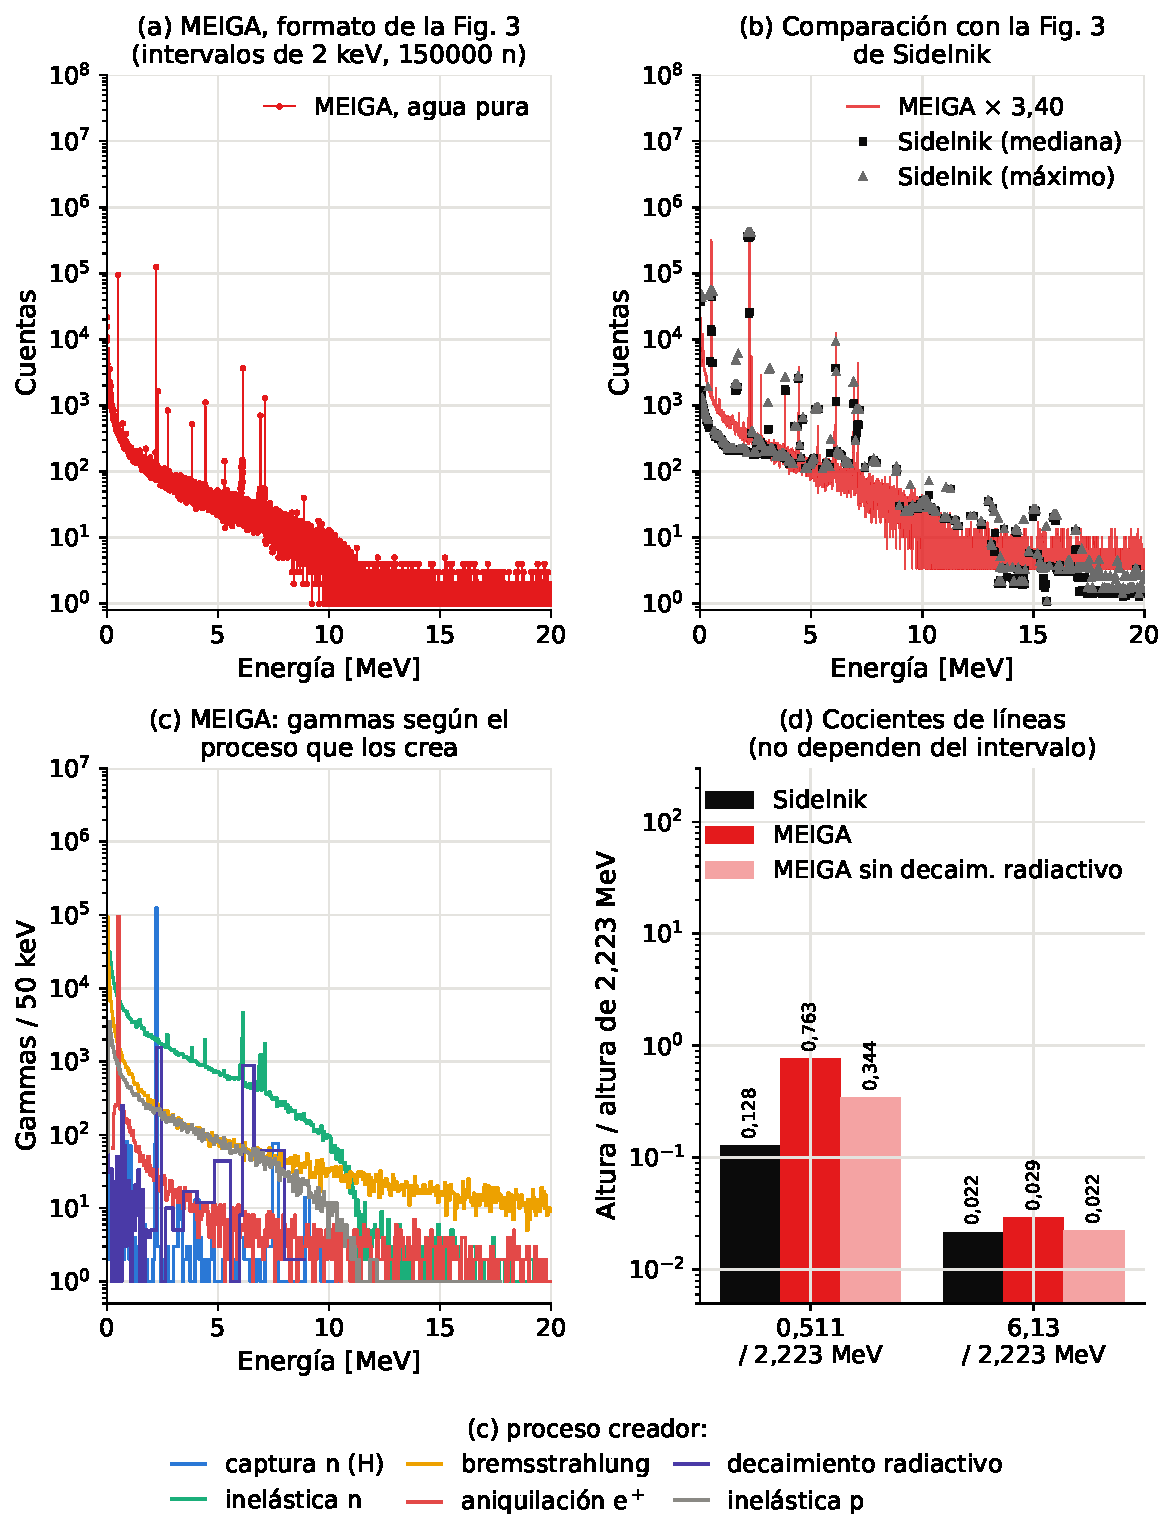
\includegraphics[width=\linewidth]{../figuras/fig11_espectro_gamma_tipo_sidelnik.pdf}\caption{(a) Espectro de energía de los gammas creados en el agua pura, en el formato de la Fig.~3 de Sidelnik. (b) MEIGA con el pico de 2,223\,MeV igualado frente a la Fig.~3 digitalizada. (c) Composición del espectro de MEIGA por proceso creador. (d) Cocientes de líneas.}\end{figure}
\paragraph{Fig. 4 de Sidelnik: gammas acumulados.} La Fig.~4 del artículo muestra los mismos gammas acumulados de derecha a izquierda, $N(\geq E)$, en bines de 1\,MeV hasta 100\,MeV (Fig.~\ref{fig:fig4}).
Se digitalizaron sus marcadores (\texttt{fig4\_gammas\_acumulados.py}); por encima de 9\,MeV las cuatro curvas del artículo se superponen y se usa su valor común.
Tres cocientes, independientes de la normalización, resumen la comparación:
\begin{itemize}
\item \textbf{Línea de 2,223\,MeV frente a los gammas de más de 3\,MeV}, $[N(\geq2)-N(\geq3)]/N(\geq3)$: 2,32 en el artículo y 1,27 en MEIGA (agua pura), un factor 1,8.
Es la misma conclusión que el salto en el borde Compton (Sec.~\ref{sec:interp_fig5}): por cada captura en H, MEIGA produce $\approx$\,1,6--1,8 veces más gammas de desexcitación nuclear. Entre 3 y 6\,MeV, donde dominan esos gammas, el cociente Sidelnik/MEIGA de las cuentas es constante ($\approx$\,1,37).
\item \textbf{Gammas de más de 20\,MeV}, $N(\geq20)/N(\geq3)$: 0,029 en el artículo, 0,163 en MEIGA y 0,0031 en MEIGA sin los eventos con piones. Los gammas de alta energía vienen casi solo de los piones
(desintegración $\pi^0\to\gamma\gamma$, con gammas de $\approx$\,70\,MeV, y bremsstrahlung de sus cascadas). El artículo queda entre las dos curvas de MEIGA: tiene piones, pero $\approx$\,6 veces menos que Bertini en Geant4\,10.7 en esta observable, lo que concuerda con la cola de la Fig.~6.
\item \textbf{Efecto del NaCl}, $N(\geq E)_{\rm NaCl}/N(\geq E)_{\rm pura}$: entre 3 y 6\,MeV vale 1,46--1,58 en MEIGA y 1,91--2,01 en el artículo (el fondo mayor de MEIGA diluye la contribución del Cl); a 8\,MeV MEIGA queda por encima (1,34 frente a 1,14) por la línea de 8,58\,MeV, y desde 9\,MeV ambos valen 1: la sal no cambia los gammas de alta energía.
\end{itemize}
\begin{figure}[H]\centering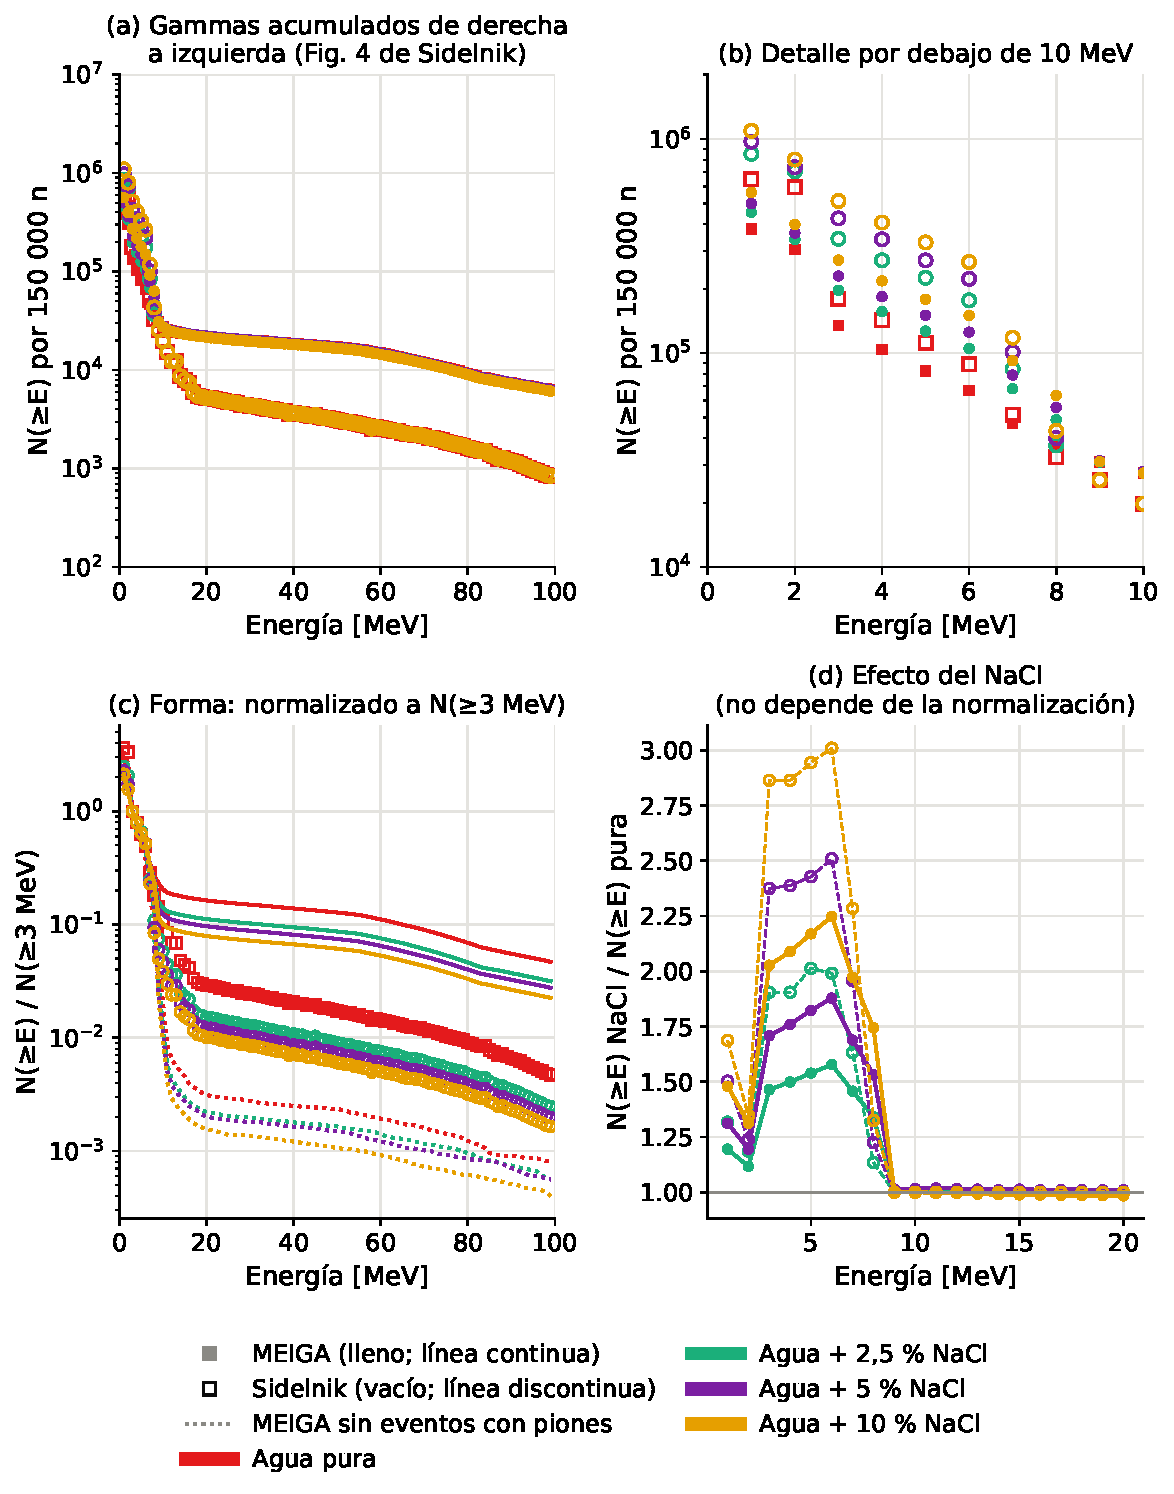
\includegraphics[width=\linewidth]{../figuras/fig17_gammas_acumulados.pdf}\caption{Gammas creados en el medio acumulados de derecha a izquierda (formato de la Fig.~4 de Sidelnik): (a) hasta 100\,MeV y (b) por debajo de 10\,MeV, MEIGA (lleno) y artículo (vacío), cuentas por 150\,000 neutrones; (c) forma normalizada a $N(\geq3\,{\rm MeV})$, con y sin los eventos con piones; (d) cociente 2,5\,\% NaCl/agua pura.}\label{fig:fig4}\end{figure}
\begin{table}[H]\centering\small\begin{adjustbox}{max width=\linewidth}\begin{tabular}{lccc}\toprule
Cociente de alturas & Sidelnik & MEIGA & MEIGA sin decaimiento radiactivo \\\midrule
0,511\,MeV / 2,223\,MeV & 0,128 & 0,763 & 0,344$^*$ \\
6,13\,MeV / 2,223\,MeV & 0,022 & 0,029 & 0,022 \\
\bottomrule
\end{tabular}\end{adjustbox}\caption{Cocientes entre las alturas de las líneas principales (agua pura). $^*$Estimado restando la fracción de positrones que vienen de desintegraciones $\beta^+$.}\end{table}
\paragraph{Línea de 2,223\,MeV y línea de 6,13\,MeV.} La línea de 6,13\,MeV del $^{16}$O la producen la dispersión inelástica de neutrones (2\,895 gammas)
y la desintegración del $^{16}$N ($T_{1/2}=7{,}1$\,s, 881 gammas), producido por $^{16}$O$(n,p)$. Sin esta última, el cociente con la línea de captura en H
es 0,022, igual al del artículo (0,022): la captura en H y la dispersión inelástica en O se reproducen con la misma proporción.
\paragraph{Línea de aniquilación (0,511\,MeV).} En MEIGA es unas 6 veces más intensa, relativa a la de 2,223\,MeV, que en el artículo.
Los positrones que la producen vienen de desintegraciones $\beta^+$ de núcleos producidos por espalación del oxígeno ($^{15}$O, $^{13}$N, $^{11}$C, con vidas medias de minutos; 55\,\%),
de conversión de gammas de alta energía en pares (39\,\%) y de la desintegración de muones positivos procedentes de $\pi^+$ (6\,\%).
Geant4 simula las desintegraciones radiactivas sin límite de tiempo; si la simulación de Sidelnik no las incluía, o las cortaba en tiempo, el cociente de MEIGA bajaría a 0,34,
y el exceso restante (unas 2,7 veces) es coherente con la mayor producción de piones encontrada en la Sec.~\ref{sec:fig6}.
\paragraph{Continuo.} Entre 2,5 y 9\,MeV la forma del continuo coincide (es la cola de la dispersión inelástica de neutrones). Por debajo de 1,5\,MeV el continuo de MEIGA es varias veces más alto,
dominado por el bremsstrahlung de electrones y positrones de alta energía, que de nuevo apunta a la producción de piones y sus cascadas.
Por encima de 10\,MeV el artículo muestra un continuo que llega hasta $\approx$\,17\,MeV, más alto que el de MEIGA, cuya componente de dispersión inelástica termina hacia 11\,MeV; con la precisión de la digitalización en esa zona
(decenas de cuentas y la curva roja parcialmente tapada) esta diferencia debe tomarse con cautela.
\aviso{En resumen: las líneas y el continuo ligados a la moderación, la captura y la dispersión inelástica de neutrones (2,223 y 6,13\,MeV, continuo de 2,5--9\,MeV) se reproducen;
las diferencias (línea de 0,511\,MeV y continuo de baja energía) se explican por el decaimiento radiactivo de larga vida y por la mayor producción de piones a 500\,MeV en el modelo de Bertini, igual que en la cola de la Fig.~6.}
\subsection{Líneas del cloro (Fig. 3 de Sidelnik)}\label{sec:cl_lineas}
\begin{table}[H]\centering\small\begin{adjustbox}{max width=\linewidth}\begin{tabular}{lcccccc}\toprule
 & \multicolumn{2}{c}{2,5\,\%} & \multicolumn{2}{c}{5\,\%} & \multicolumn{2}{c}{10\,\%} \\
Línea [MeV] / 2,223\,MeV & Sidelnik & MEIGA & Sidelnik & MEIGA & Sidelnik & MEIGA \\\midrule
0{,}511/0{,}517 & 0,423 & 1,305 & 0,678 & 1,788 & 1,181 & 2,796 \\
1{,}165 (Cl) & 0,165 & 0,147 & 0,312 & 0,277 & 0,574 & 0,561 \\
1{,}951 (Cl) & 0,179 & 0,104 & 0,339 & 0,200 & 0,624 & 0,397 \\
6{,}11/6{,}13 & 0,115 & 0,109 & 0,217 & 0,212 & 0,412 & 0,425 \\
7{,}41 (Cl) & 0,059 & 0,057 & 0,112 & 0,107 & 0,206 & 0,216 \\
7{,}79 (Cl) & 0,047 & 0,046 & 0,089 & 0,084 & 0,165 & 0,172 \\
8{,}58 (Cl) & 0,016 & 0,151 & 0,029 & 0,292 & 0,054 & 0,583 \\
\bottomrule\end{tabular}\end{adjustbox}\caption{Altura de las líneas respecto a la de 2,223\,MeV en los medios con NaCl. La digitalización (25,6\,keV por píxel) no separa 0,511/0,517 ni 6,11/6,13\,MeV.}\end{table}
Las líneas de la cascada del $^{36}$Cl de 1,165, 6,11, 7,41 y 7,79\,MeV coinciden con el artículo dentro del 3--10\,\%: la proporción de capturas en Cl respecto a H y la intensidad de esas transiciones
son las mismas en las dos simulaciones. La línea de 1,951\,MeV queda algo por debajo (en la figura del artículo se superpone con la de 1,959\,MeV).
Hay dos diferencias: la línea de 0,511\,MeV, más intensa por las mismas causas que en agua pura (emisores $\beta^+$ de larga vida y piones), y la de 8,58\,MeV, unas 10 veces más intensa en MEIGA.
\begin{figure}[H]\centering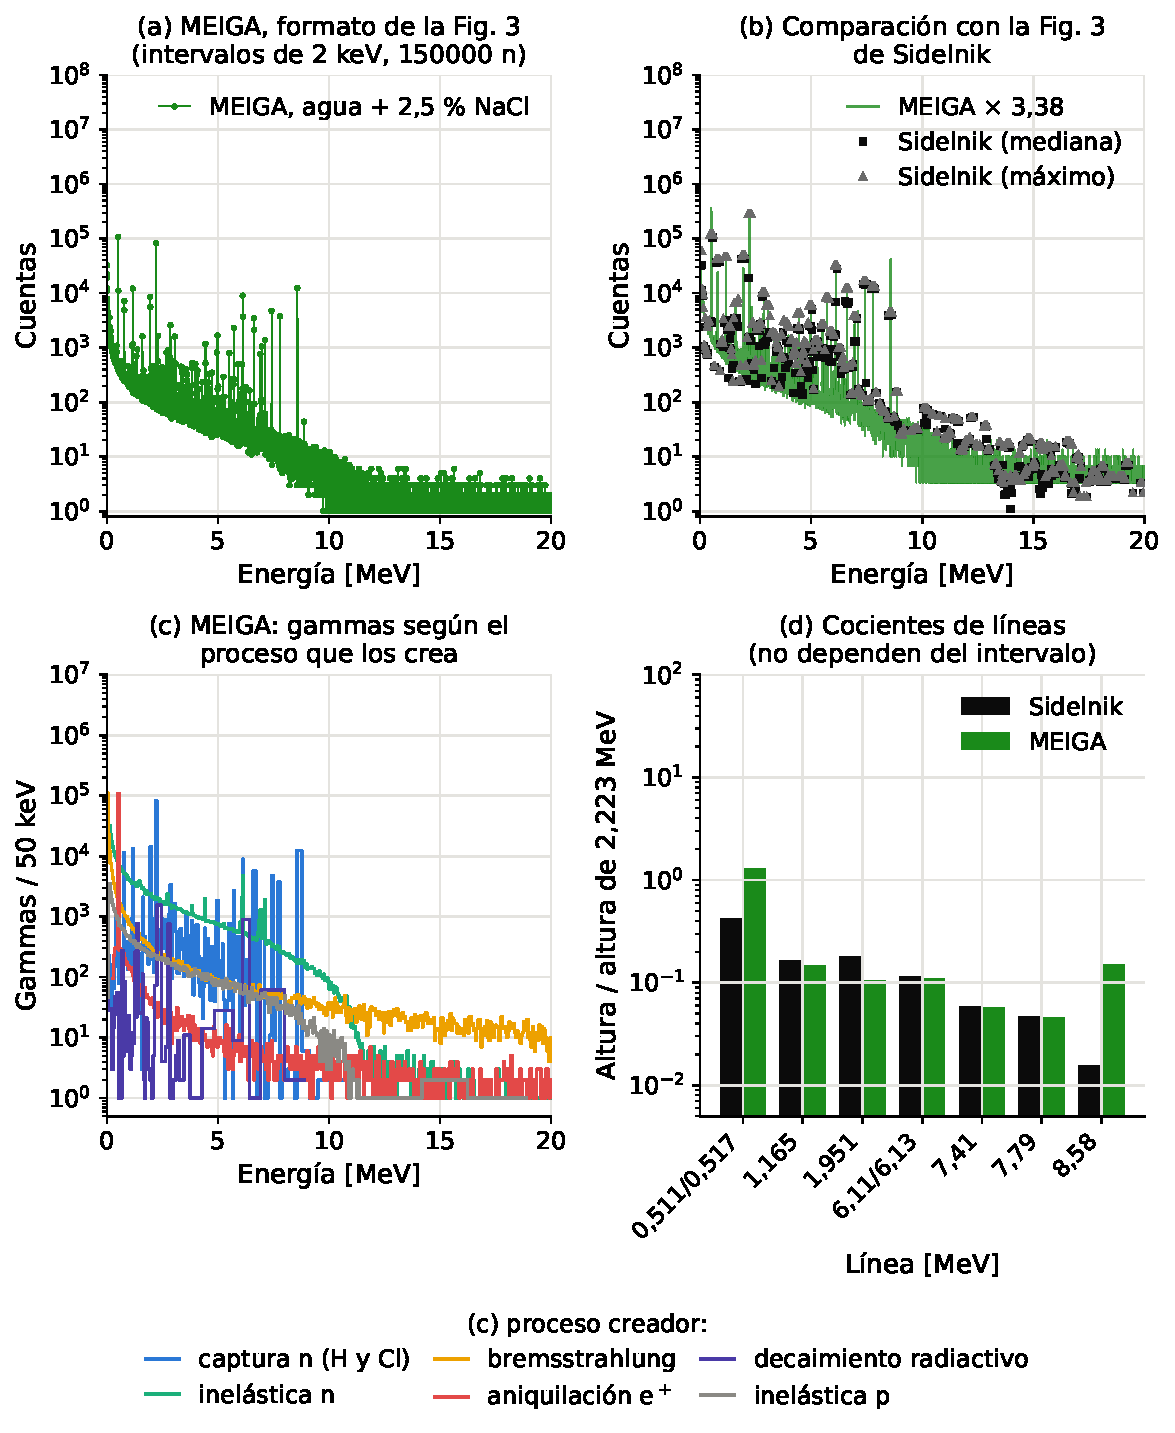
\includegraphics[width=\linewidth]{../figuras/fig11_espectro_gamma_tipo_sidelnik_nacl25.pdf}\caption{Espectro gamma en agua + 2,5\,\% NaCl: (a) formato de la Fig.~3 de Sidelnik; (b) comparación con su curva digitalizada; (c) composición por proceso; (d) cocientes de las líneas con la de 2,223\,MeV.}\end{figure}

\section{Comparación de los espectros de electrones y positrones secundarios}
{\small\textit{Corresponde a la Sec.~4.1.1.4 de la tesis (Fig. 4.5).}}

\subsection{Electrones creados por gammas}
\begin{figure}[H]\centering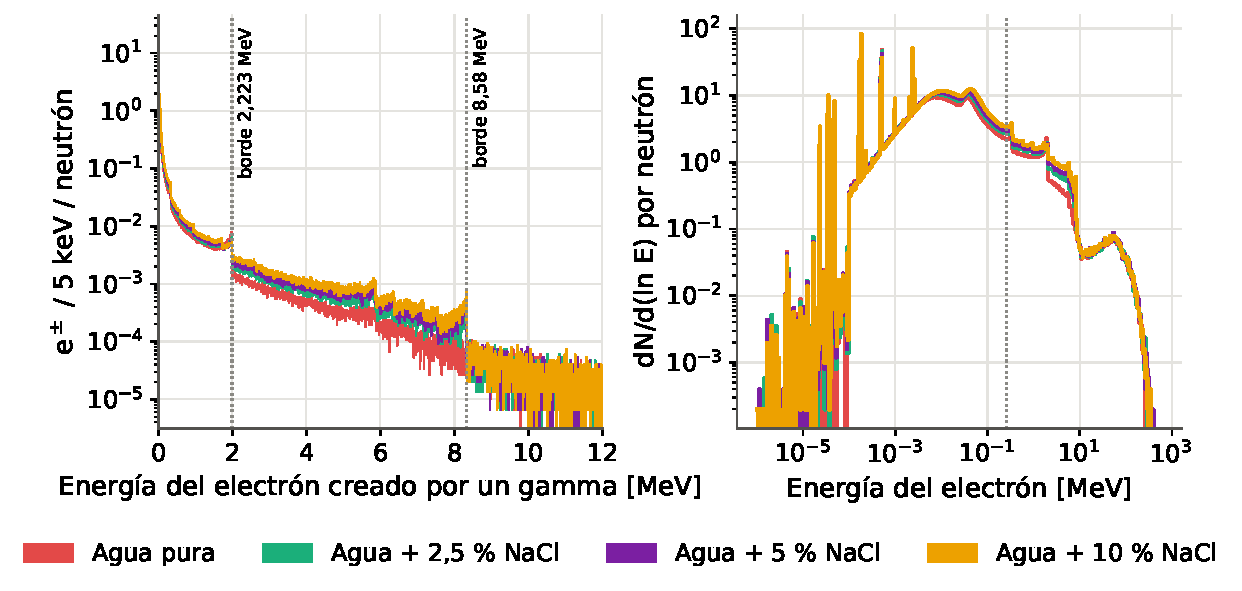
\includegraphics[width=\linewidth]{../figuras/fig03_espectro_electrones.pdf}\caption{Electrones creados por gammas en el agua (como la Fig.~5 de Sidelnik), con el borde Compton de 1,994\,MeV de la línea de 2,223\,MeV; derecha, en escala logarítmica.}\end{figure}
\subsubsection{Comparación con la Fig. 5 de Sidelnik: electrones producidos por gammas}\label{sec:fig5}
Se sumaron los electrones que crean los gammas en el agua por efecto Compton, fotoeléctrico y producción de pares (\texttt{secundarias-interaccion-gamma.tsv}),
con bines de 20\,keV y cuentas escaladas a 150\,000 neutrones, y se compararon con la Fig.~5 del artículo digitalizada por color (\texttt{digitalizar\_fig5.py}).
\paragraph{Escala absoluta.} A diferencia de las Figs.~3 y 6, aquí no hace falta ninguna normalización: ambas figuras son electrones por 150\,000 neutrones con bines de 20\,keV.
El factor $k$ de la figura siguiente (panel b) es la mediana del cociente Sidelnik/MEIGA en 11 energías entre 0,5 y 7\,MeV: 1,06 (agua pura), 1,09 (2,5\,\%), 1,07 (5\,\%), 1,04 (10\,\%).
Es decir, MEIGA produce entre un 4 y un 8\,\% menos de electrones que la simulación del artículo, y su forma coincide desde 0,3 hasta 10\,MeV.
Este factor vale solo para los electrones: el de la Fig.~3 (3,40) es una normalización, porque el eje de Sidelnik está en unidades arbitrarias (Sec.~\ref{sec:fig3}).
\paragraph{Por qué MEIGA tiene menos electrones.} (i) La causa principal es que Sidelnik tiene más capturas: el cociente de probabilidades de captura Sidelnik/MEIGA es
1,05, 1,09, 1,10, 1,12 (mismo orden de medios), prácticamente igual a $k$ en agua pura y con 2,5\,\%.
Con 5 y 10\,\% $k$ queda por debajo de ese cociente porque cada captura en Cl de MEIGA emite más energía de la real (10,1 frente a 8,58\,MeV; Sec.~\ref{sec:cascadas_cl}) y produce más electrones, lo que compensa en parte las capturas que faltan.
(ii) $k$ es un promedio: punto a punto el cociente va de 0,85 a 1,35 en agua pura; Sidelnik está más alto justo debajo del borde de 1,994\,MeV y MEIGA entre 2 y 3\,MeV, donde domina el fondo de desexcitación nuclear (Sec.~\ref{sec:interp_fig5}),
y con NaCl MEIGA queda muy por encima entre 7,4 y 8,3\,MeV por el gamma único de 8,58\,MeV. (iii) La digitalización por color en escala logarítmica tiene una incertidumbre del 5--10\,\%.
(iv) Las versiones de Geant4 y las listas físicas son distintas y el artículo no las especifica. La diferencia de amplitud es, por tanto, pequeña y se explica casi por completo por la probabilidad de captura;
las diferencias físicamente relevantes están en la forma (fondo de desexcitación nuclear y gamma único de 8,58\,MeV).
\paragraph{Bordes Compton.} Se ven en ambas simulaciones los bordes de la línea de aniquilación (0,34\,MeV), de la captura en H (1,994\,MeV) y de la línea de 6,13/6,11\,MeV (5,87\,MeV).
El salto en el borde de 1,994\,MeV (nivel antes/después) es 4,5 en MEIGA y 6,5 en el artículo; el de 5,87\,MeV, 1,74 y 1,63.
\paragraph{Efecto del NaCl.} El cociente 2,5\,\% NaCl/agua pura no depende de la normalización. Por debajo de 1,9\,MeV es $\approx$\,1,1 en ambas simulaciones; entre 2 y 6\,MeV, donde contribuyen los electrones Compton de las líneas del Cl,
vale 1,42--1,96 en MEIGA y 1,63--2,19 en el artículo.
Las diferencias aparecen por encima de 7\,MeV: el borde Compton de la línea de 8,58\,MeV (8,33\,MeV) produce en MEIGA un salto de 5,6 frente a 1,8 en el artículo,
consecuencia directa del exceso de transiciones directas al fundamental en las cascadas del $^{35}$Cl de Geant4 (Sec.~\ref{sec:nacl25}). Los bordes de 7,17 y 7,54\,MeV (líneas de 7,41 y 7,79\,MeV) tienen saltos parecidos en las dos simulaciones.
\begin{figure}[H]\centering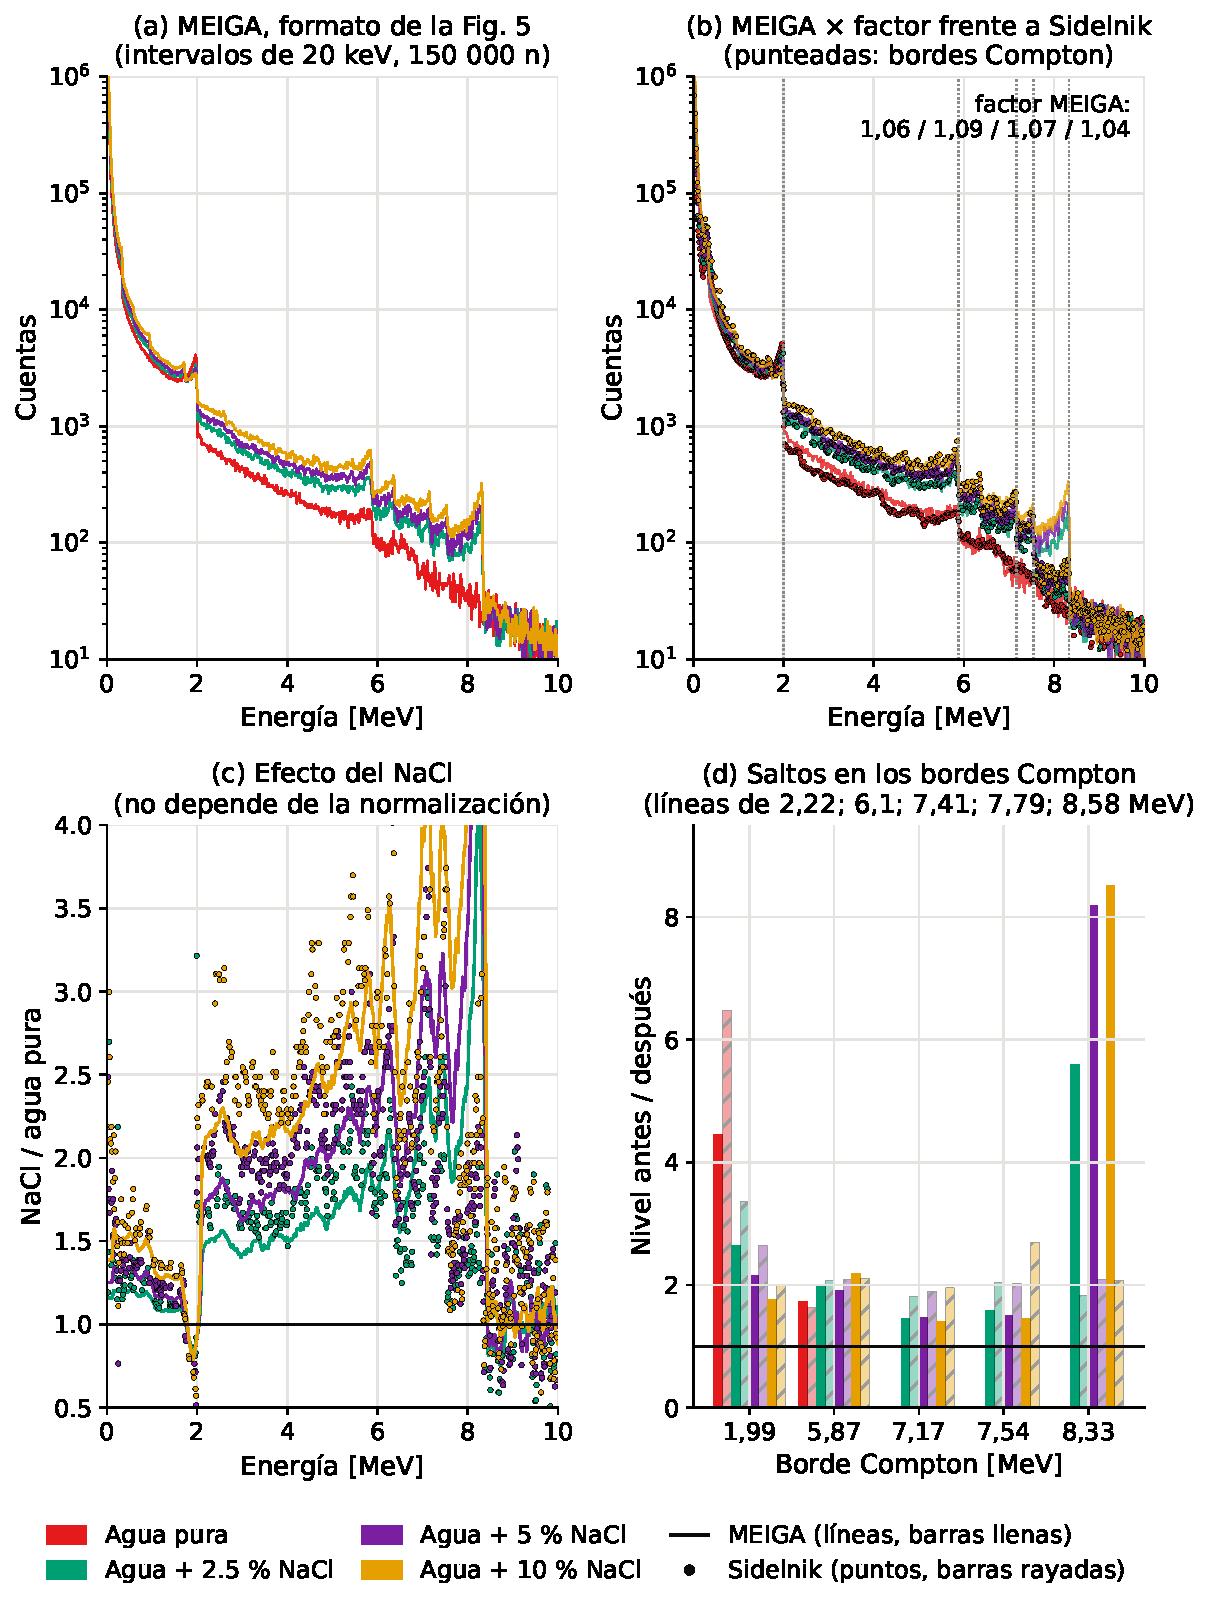
\includegraphics[width=\linewidth]{../figuras/fig13_espectro_electrones_tipo_sidelnik.pdf}\caption{Electrones producidos por gammas en el agua: (a) formato de la Fig.~5 de Sidelnik (bines de 20\,keV, 150\,000 neutrones); (b) MEIGA frente a la figura digitalizada, con los bordes Compton; (c) cociente NaCl/agua pura; (d) saltos en los bordes Compton.}\end{figure}
\subsubsection{Interpretación física de las diferencias con la Fig. 5}\label{sec:interp_fig5}
Para entender las diferencias se clasificó cada electrón según el origen del gamma que lo produce (\texttt{origen\_electrones.py}): el electrón se enlaza con su gamma padre
(\texttt{pasos-gamma.tsv}), el gamma con su proceso creador y, si es de captura, con el núcleo que capturó el neutrón (\texttt{capturas-neutrones.tsv}). Fig.~\ref{fig:origen}.
\paragraph{El salto en el borde de 1,994\,MeV mide la razón captura en H / fondo.} Por debajo del borde, el 76\,\% de los electrones viene de la línea de 2,223\,MeV;
por encima, el 78\,\% viene de gammas de la dispersión inelástica de neutrones en el oxígeno (desexcitación de $^{16}$O$^*$, $^{12}$C$^*$, $^{15}$N$^*$: líneas de 4,44, 6,13, 6,92, 7,12\,MeV y su continuo).
El salto vale, por tanto, $J \approx 1 + C_H/F$, con $C_H$ los electrones de la captura en H y $F$ ese fondo. Los piones no son la causa: sin los eventos con piones el salto apenas pasa de 4,46 a 4,58.
Para obtener el salto de Sidelnik (6,5) habría que dividir el fondo de MEIGA por 1,60 en agua pura y por 1,76 con 2,5\,\% NaCl:
el mismo factor en los dos medios, como corresponde a un fondo que no depende de la sal. Es decir, por cada captura en H, MEIGA produce $\approx$\,1,6 veces más gammas de desexcitación nuclear que la simulación del artículo.
Esto concuerda con el espectro gamma: respecto a la línea de 2,223\,MeV, las líneas de 6,13\,MeV ($^{16}$O) y 4,44\,MeV ($^{12}$C) son 1,35 y 1,40 veces más intensas en MEIGA (las demás quedan tapadas en la figura digitalizada),
y Sidelnik tiene además $\approx$\,5\,\% más capturas (25,18 frente a 24,08\,\%). El salto en el borde de 5,87\,MeV, que mide justamente la línea de 6,13\,MeV, es por la misma razón algo mayor en MEIGA (1,74 frente a 1,63).
La producción de gammas en la dispersión inelástica de neutrones de 10--500\,MeV depende del modelo de cascada (Bertini por encima de $\approx$\,20\,MeV) y de la desexcitación de los núcleos residuales (\texttt{G4PhotonEvaporation}, datos G4NDL por debajo de 20\,MeV),
que cambiaron entre versiones de Geant4; sin conocer la versión y la lista física de Sidelnik no se puede atribuir la diferencia a un componente concreto.
\paragraph{El cociente NaCl/agua pura.} Con NaCl el cociente vale $1 + C_{Cl}/F$ en la región de 2--6\,MeV, donde solo contribuyen las capturas en Cl y el fondo. Hay tres efectos:
\begin{enumerate}
\item Debajo del borde de 1,994\,MeV el cociente baja a $\approx$\,0,84 en las dos simulaciones: el Cl compite con el H y las capturas en H por neutrón caen de 0,83 a 0,55. Que el valor coincida indica que la competencia H/Cl es parecida en ambas.
\item Entre 2 y 6\,MeV el fondo más alto de MEIGA diluye la contribución del Cl, y el cociente queda por debajo del de Sidelnik (1,49 frente a 1,63 entre 2 y 4\,MeV).
Si se divide el fondo por el mismo factor 1,60, el cociente pasa a 1,75 y 2,07, algo por encima del artículo (1,63 y 1,74):
una vez corregido el fondo, los electrones de las capturas en Cl de MEIGA son $\approx$\,1,2--1,4 veces los del artículo. Es lo esperado de los dos defectos de Geant4 ya identificados: $\approx$\,1,27 veces más capturas en Cl que las secciones eficaces térmicas
y cascadas con 10,2\,MeV en promedio en vez de 8,58\,MeV.
\item Entre 7 y 8,3\,MeV el cociente de MEIGA (2,46) supera al del artículo (1,58) por los electrones Compton de la línea de 8,58\,MeV: el 24\,\% de las capturas en $^{35}$Cl emite un único gamma de 8,58\,MeV, frente a $\approx$\,3\,\% en la naturaleza.
\end{enumerate}
\aviso{Las intensidades relativas de las líneas intermedias del Cl (1,165, 6,11, 7,41, 7,79\,MeV) coinciden con Sidelnik porque los dos defectos se compensan: hay $\approx$\,1,27 veces más capturas en Cl,
pero solo $\approx$\,76\,\% de ellas siguen una cascada (el resto va directo al fundamental); $1{,}27 \times 0{,}76 \approx 0{,}97$. En la luz total, en cambio, los defectos se suman, porque cada captura en Cl deposita más energía de la debida.}
\begin{figure}[H]\centering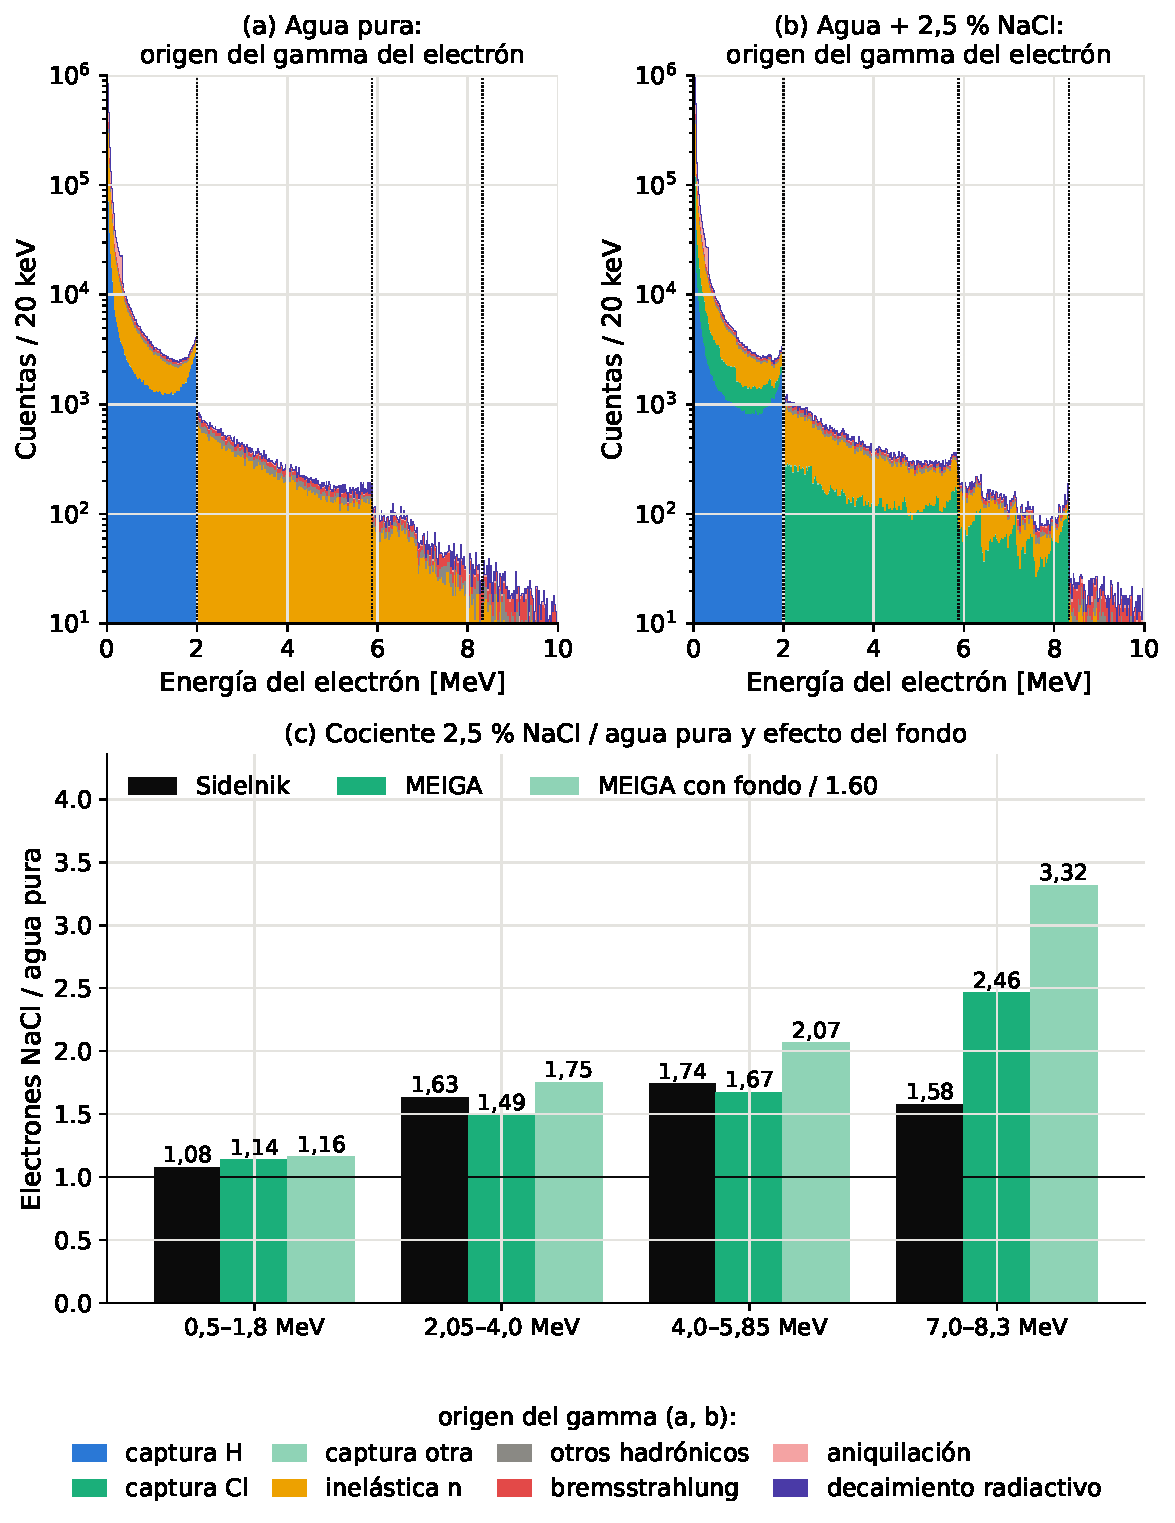
\includegraphics[width=\linewidth]{../figuras/fig14_origen_electrones.pdf}\caption{Origen del gamma que produce cada electrón (agua pura y 2,5\,\% NaCl; áreas apiladas) y cociente NaCl/agua pura en cuatro intervalos: Sidelnik, MEIGA y MEIGA con el fondo no debido a capturas dividido por el factor que reproduce el salto de 1,994\,MeV del artículo.}\label{fig:origen}\end{figure}

\section{Distribución de energía de los deuterones producidos en la captura de neutrones sobre hidrógeno}
{\small\textit{Corresponde a la Sec.~4.1.1.5 de la tesis (Fig. 4.6).}}

\subsection{Deuterones de la captura en H (Fig. 4.6 de la tesis)}\label{sec:deut}
En la captura $n + p \to d + \gamma$ el deuterón retrocede con $E_d \simeq E_\gamma^2/(2M_dc^2) = 2{,}2244^2/(2\times1875{,}6)$\,MeV $=1,319$\,keV.
La distribución de MEIGA (Fig.~\ref{fig:deut}) tiene su máximo exactamente ahí (mediana 1,319\,keV) y una anchura $\sigma = 9,9$\,eV,
que viene del movimiento térmico del neutrón y del protón en el instante de la captura (la misma causa que da a la línea de 2,224\,MeV su anchura de 0,013\,keV).
Las alturas coinciden con la Fig.~4.6: con la sal el pico baja a $\approx$\,0,66 veces el de agua pura porque solo el 64\,\% de las capturas ocurre en H.
La media y el RMS que se citan en la Fig.~4.6 no describen el pico: los dominan unos pocos deuterones (0,12\,\%) de capturas de neutrones aún rápidos, con energías de hasta 6,9\,MeV;
MEIGA da media 1,43\,keV y RMS 23,2\,keV en agua pura (tesis: 1,48 y 31,3\,keV). Para describir el pico conviene citar la mediana y la $\sigma$ en la ventana de 1,20--1,45\,keV
(1,319\,keV y 9,9\,eV en agua pura; 1,319\,keV y 10,5\,eV con 2,5\,\% NaCl; 1,319\,keV y 10,8\,eV con 5\,\% NaCl; 1,319\,keV y 11,6\,eV con 10\,\% NaCl): la mediana no depende del medio y la anchura crece ligeramente con la sal.
\begin{figure}[H]\centering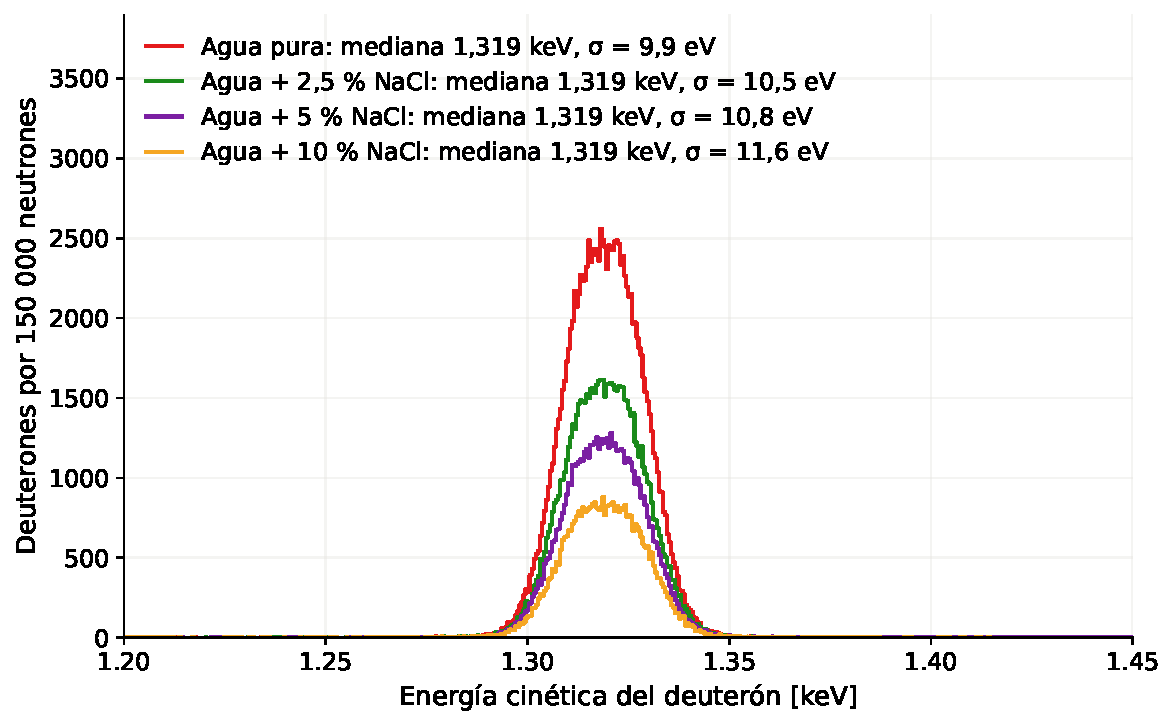
\includegraphics[width=0.85\linewidth]{../figuras/fig16_deuterones_captura.pdf}\caption{Energía de los deuterones producidos en la captura $^1$H(n,$\gamma$)$^2$H (formato de la Fig.~4.6 de la tesis); cuentas por 150\,000 neutrones primarios.}\label{fig:deut}\end{figure}

\section{Comparación de la distribución de fotones Cherenkov detectados para neutrones de 500 MeV}
{\small\textit{Corresponde a la Sec.~4.1.1.6 de la tesis (Fig. 4.7).}}

\subsection{Fotones Cherenkov y carga en el PMT (Fig. 6 de Sidelnik)}
\begin{table}[H]\centering\small\begin{adjustbox}{max width=\linewidth}\begin{tabular}{lcccc}\toprule
 & Agua pura & 2,5\,\% NaCl & 5\,\% NaCl & 10\,\% NaCl \\\midrule
Fotones Cherenkov creados por neutrón & 1\,441 & 1\,662 & 1\,806 & 1\,994 \\
Carga media [p.e.] & 9,78 & 11,38 & 12,42 & 13,89 \\
Eventos con $Q\geq 1$ & 53,0\,\% & 54,9\,\% & 56,0\,\% & 58,1\,\% \\
p.e. por fotón creado & 0,68\,\% & 0,68\,\% & 0,69\,\% & 0,70\,\% \\
Carga $<1$\,µs & 85,7\,\% & 75,6\,\% & 71,7\,\% & 67,4\,\% \\
Carga 1\,µs--1\,ms (capturas) & 12,7\,\% & 22,9\,\% & 26,9\,\% & 31,1\,\% \\
Carga $>1$\,ms (desintegraciones) & 1,55\,\% & 1,49\,\% & 1,45\,\% & 1,50\,\% \\
\bottomrule\end{tabular}\end{adjustbox}\caption{Producción de luz Cherenkov y respuesta del PMT.}\end{table}
\aviso{La distribución de fotoelectrones de MEIGA es mucho más estrecha que la Fig.~6 de Sidelnik: la media es 9,8\,p.e.
y casi no hay eventos por encima de 400\,p.e., mientras que la curva del artículo se extiende hasta $\sim$1000. Se crean unos 1\,441 fotones Cherenkov por neutrón
y llega al PMT (tras la eficiencia cuántica) el 0,68\,\%. La Sec.~\ref{sec:diag} muestra que la diferencia indica que la Fig.~6 del artículo no incluye la colección óptica (el artículo no lo especifica); la Fig.~6 digitalizada tiene además los problemas descritos en el informe v0.6.0.
Como en las corridas anteriores, Geant4 simula desintegraciones radiactivas sin límite de tiempo: el 1,55\,\% de la carga llega después de 1\,ms.}
\begin{figure}[H]\centering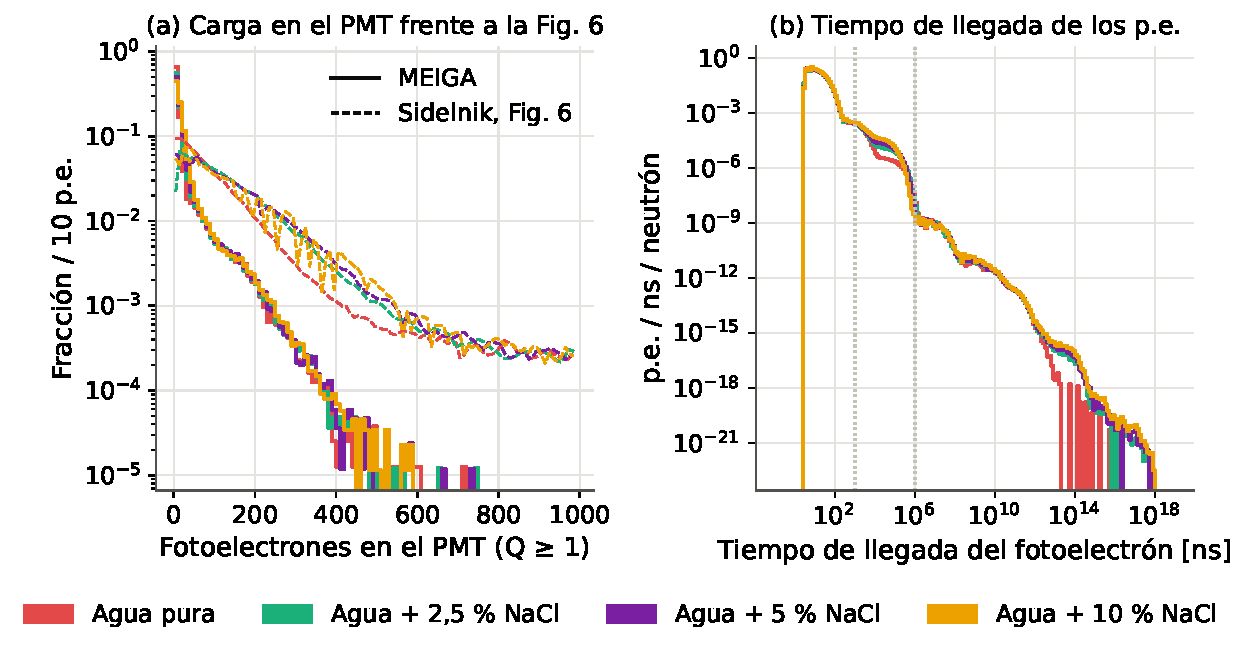
\includegraphics[width=\linewidth]{../figuras/fig04_carga_y_tiempos.pdf}\caption{Distribución de fotoelectrones en el PMT frente a la Fig.~6 de Sidelnik (digitalizada) y tiempos de llegada de los fotoelectrones.}\end{figure}
\begin{figure}[H]\centering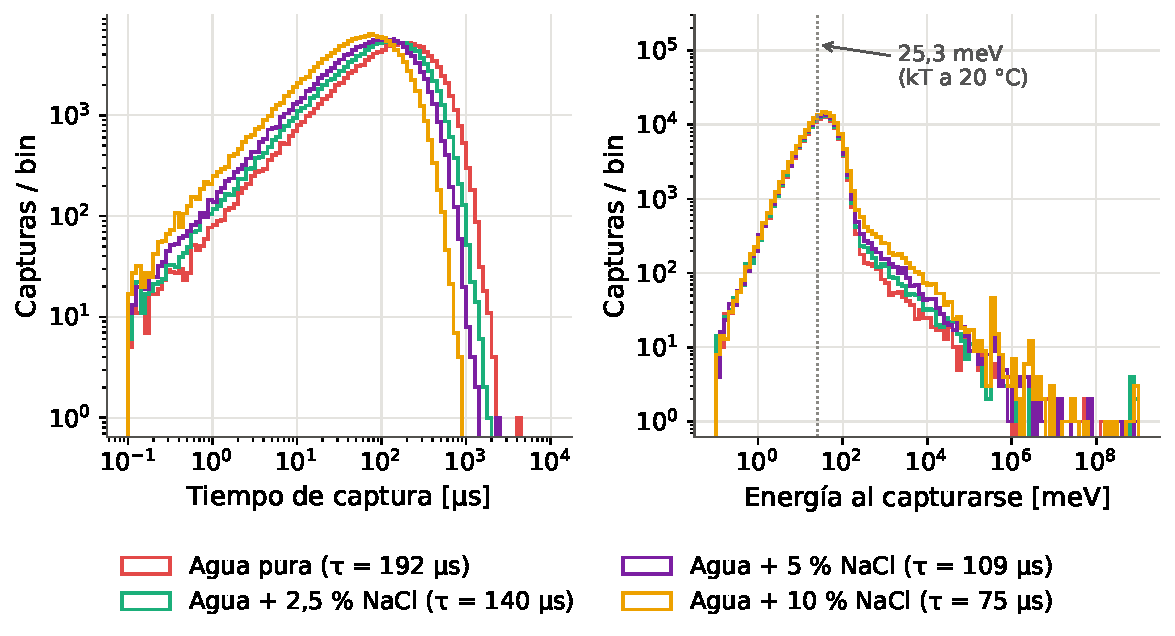
\includegraphics[width=\linewidth]{../figuras/fig05_tiempo_energia_captura.pdf}\caption{Tiempo de captura y energía del neutrón al capturarse.}\end{figure}
\subsection{La Fig. 6 de Sidelnik reproducida con MEIGA y el histograma de carga}\label{sec:fig6}
\subsubsection{Procedimiento}
Para comparar con la Fig.~6 del artículo se usa su mismo observable. Para cada uno de los 150\,000 neutrones:
\begin{enumerate}
\item Se cuentan los fotones Cherenkov aceptados por la eficiencia cuántica del PMT en el momento de crearse, sin transporte óptico. En el modo \texttt{eFast} de MEIGA son exactamente los fotones que el simulador transporta, por lo que se obtienen de \texttt{pasos-particulas.tsv}.
\item Se descartan los eventos sin ningún fotón aceptado (39,0\,\% de los neutrones), porque la Fig.~6 no muestra el pico en cero.
\item Se histograma como en el artículo: bines de 10 fotones, eje de 0 a 2500 fotones, escala logarítmica y cuentas absolutas, sin normalizar ni reescalar.
\end{enumerate}
Las curvas digitalizadas de la Fig.~6 se limpiaron de dos artefactos de la digitalización: la leyenda capturada entre 1590 y 1800 fotones y el borde final del eje en las curvas con NaCl.
\begin{figure}[H]\centering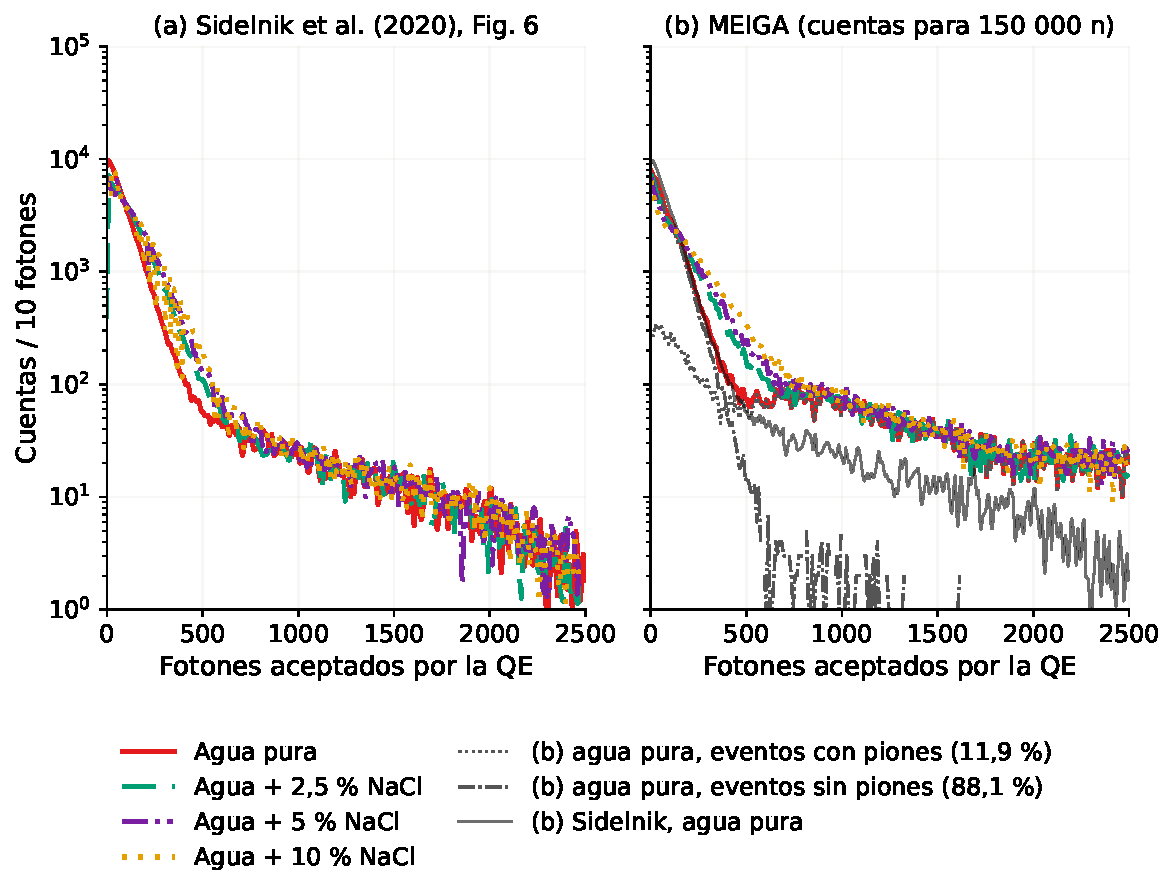
\includegraphics[width=\linewidth]{../figuras/fig10_figura6_sidelnik_vs_meiga.pdf}\caption{Izquierda: Fig.~6 de Sidelnik et al.\ (2020), digitalizada. Derecha: la misma figura construida con MEIGA para agua pura (150\,000 neutrones de 500\,MeV), con la curva de Sidelnik superpuesta y los eventos separados según haya o no producción de piones en una interacción inelástica del neutrón.}\end{figure}
\begin{table}[H]\centering\small\begin{adjustbox}{max width=\linewidth}\begin{tabular}{lrrr}\toprule
Fotones aceptados & MEIGA & Sidelnik (digitalizada) & MEIGA/Sidelnik \\\midrule
0--100 & 52\,395 & 67\,941 & 0,77 \\
100--500 & 28\,902 & 30\,773 & 0,94 \\
500--1000 & 3\,748 & 1\,758 & 2,13 \\
1000--2500 & 4\,783 & 1\,495 & 3,20 \\
\bottomrule\end{tabular}\end{adjustbox}\caption{Cuentas absolutas por intervalo de fotones aceptados (agua pura, eventos con al menos un fotón). Además, MEIGA tiene 1\,705 eventos por encima de 2500 fotones, fuera del eje del artículo.}\end{table}
\subsubsection{Resultado: coincidencia hasta 500 fotones}
Entre 0 y 500 fotones la distribución de MEIGA coincide con la de Sidelnik sin ningún reescalamiento: la pendiente es la misma, el quiebre aparece en 400--500 fotones como en el artículo,
y las cuentas absolutas coinciden dentro del 6--23\,\%. La correlación de la forma en escala logarítmica entre 0 y 1000 fotones es 0,985.
Esto indica que el número de neutrones, la eficiencia cuántica y la producción de luz Cherenkov son comparables en las dos simulaciones.
La mediana de MEIGA es de 22 fotones aceptados por neutrón y la media de 156 (la media está dominada por la cola).
\subsubsection{La cola por encima de 500 fotones: producción de piones}
Por encima de 500 fotones MEIGA tiene entre 2 y 3 veces más eventos que el artículo. Para identificar su origen se marcó cada evento según el archivo
\texttt{secundarias-inelastica-neutron.tsv}: un evento ``con piones'' es aquel en que alguna interacción inelástica de un neutrón produjo un $\pi^\pm$ o un $\pi^0$.
\begin{table}[H]\centering\small\begin{adjustbox}{max width=\linewidth}\begin{tabular}{lrccc}\toprule
Fotones aceptados & Eventos & Con $\pi^\pm$ & Con $\pi^0$ & Con algún pion \\\midrule
1--100 & 52\,395 & 4,0\,\% & 1,5\,\% & 5,5\,\% \\
100--500 & 28\,902 & 13,5\,\% & 2,6\,\% & 16,1\,\% \\
500--1000 & 3\,748 & 68,6\,\% & 26,5\,\% & 95,1\,\% \\
1000--2500 & 4\,781 & 35,5\,\% & 63,1\,\% & 98,6\,\% \\
$\geq$2500 & 1\,707 & 9,7\,\% & 89,3\,\% & 98,8\,\% \\
\bottomrule\end{tabular}\end{adjustbox}\caption{Fracción de eventos con producción de piones según el número de fotones aceptados (agua pura). Un mismo evento puede tener piones cargados y neutros.}\end{table}
Solo el 11,9\,\% de los neutrones produce piones (7,0\,\% con $\pi^\pm$ y 4,9\,\% con $\pi^0$),
pero esos eventos forman la cola: el 97,3\,\% de los eventos con 500 fotones o más tiene piones. Un evento con piones produce en promedio
944 fotones aceptados, frente a 49 en uno sin piones. Los $\pi^\pm$ emiten luz Cherenkov directamente a lo largo de su trayectoria
y, al desintegrarse, dan muones que también la emiten; los $\pi^0$ se desintegran en dos gammas de unos 70\,MeV que inician cascadas electromagnéticas. Entre 500 y 1000 fotones dominan los $\pi^\pm$ y por encima de 1000 los $\pi^0$.
Sin los eventos con piones, la distribución cae a cero hacia 600 fotones (la fracción de eventos con 500 fotones o más pasa de 6,8\,\% a 0,21\,\%).

\aviso{Interpretación de la cola. La energía de 500\,MeV está apenas por encima del umbral de producción de piones en colisiones nucleón--nucleón ($\approx$\,290\,MeV),
donde la sección eficaz de producción depende mucho del modelo hadrónico. MEIGA usa el modelo de cascada de Bertini (\texttt{QGSP\_BERT\_HP}, Geant4 10.7.p04).
La explicación más probable es que la simulación de Sidelnik usara otra lista física u otra versión de Geant4 que produce entre 2 y 3 veces menos piones a esta energía.
Esto no se ha comprobado: habría que conocer la versión de Geant4 y la lista física que se usaron en el artículo. En cualquier caso, la cola no afecta el tramo de 0 a 500 fotones,
que corresponde a la moderación y la captura, el objeto de estudio.}
\subsection{Efecto del NaCl en la luz Cherenkov (Fig. 6 de Sidelnik)}
Con el mismo observable de la Sec.~\ref{sec:fig6} (fotones aceptados por la eficiencia cuántica, antes del transporte óptico), MEIGA reproduce el efecto del NaCl que muestra la Fig.~6:
las curvas con NaCl quedan por encima de la de agua pura, más cuanto mayor es la concentración, entre $\approx$\,150 y 550 fotones (Fig.~\ref{fig:fig6nacl}), por la luz adicional de las capturas en Cl, y por encima de 600 fotones las dos curvas coinciden (piones).
Entre 100 y 500 fotones las cuentas aumentan 2,5\,\%: +30,1\,\% en MEIGA y +52,9\,\% en el artículo; 5\,\%: +42,8\,\% en MEIGA y +66,9\,\% en el artículo; 10\,\%: +59,2\,\% en MEIGA y +53,9\,\% en el artículo;
la correlación de forma con la curva correspondiente de Sidelnik es 0,989, 0,994, 0,982.
Los fotones Cherenkov creados por neutrón pasan de 1\,441 (agua pura) a 1\,662 (2,5\,\%), 1\,806 (5\,\%), 1\,994 (10\,\%),
y la carga media de 9,78 a 11,38, 12,42, 13,89\,p.e. (+16,4\,\%, +27,0\,\%, +42,0\,\%).
\begin{figure}[H]\centering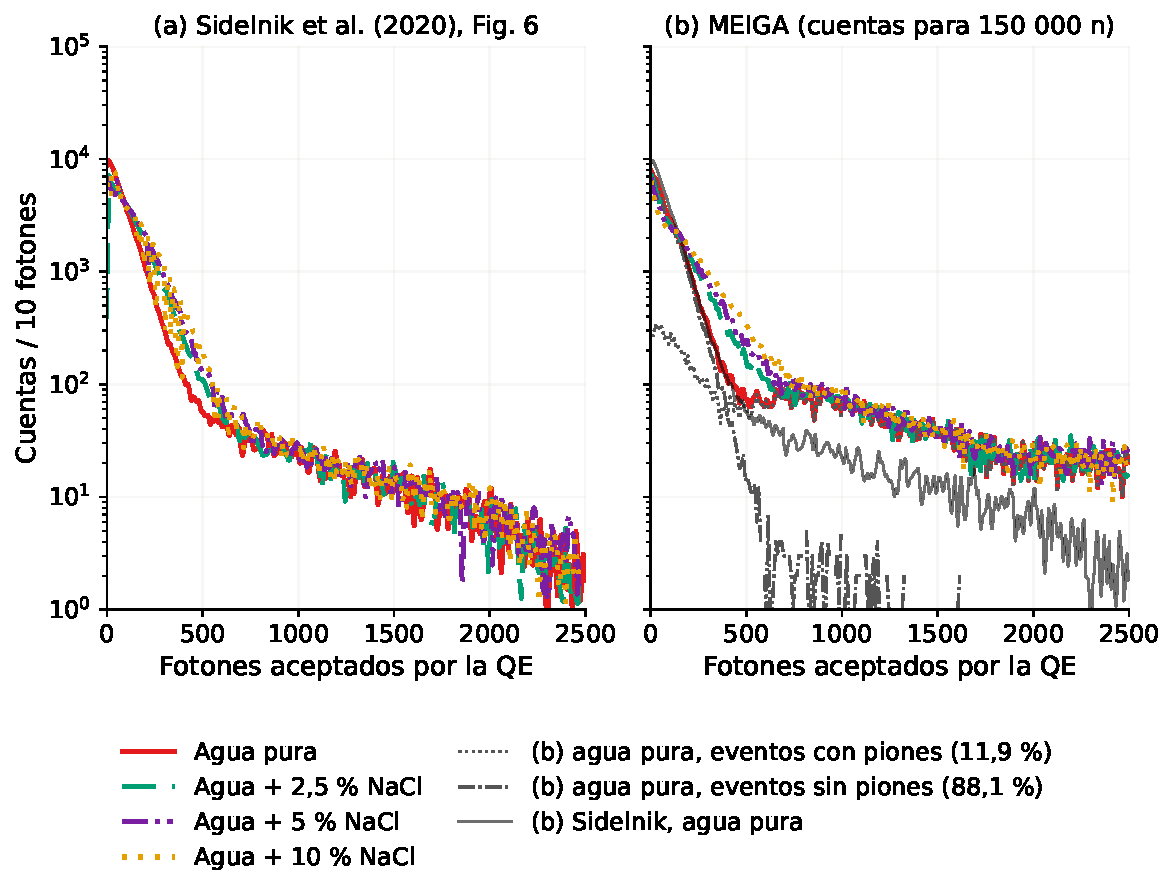
\includegraphics[width=\linewidth]{../figuras/fig10_figura6_sidelnik_vs_meiga.pdf}\caption{Fig.~6 de Sidelnik (izquierda) y MEIGA (derecha) en todos los medios simulados; 150\,000 neutrones en cada medio.}\label{fig:fig6nacl}\end{figure}
\paragraph{¿Cuánto del déficit se debe a los piones?} Se marcó cada neutrón cuyo árbol contiene una inelástica con producción de $\pi^\pm$ o $\pi^0$ (\texttt{piones\_efecto\_nacl.py}): son el 11,9\,\%, 11,9\,\%, 12,1\,\%, 12,0\,\% de los eventos (agua pura, 2,5\,\%, 5\,\%, 10\,\%), igual en todos los medios.
Sin esos eventos el aumento de cuentas entre 100 y 500 fotones pasa de 30,1 a 33,5\,\% (2,5\,\%), 42,8 a 48,8\,\% (5\,\%), 59,2 a 68,7\,\% (10\,\%), frente a 52,9\,\%, 66,9\,\%, 53,9\,\% en el artículo.
Los piones explican, por tanto, solo una parte del déficit con 2,5 y 5\,\% (unos 3 y 6 puntos de los 23 y 24 que faltan): el exceso de cuentas que aporta la sal casi no cambia al quitarlos, lo que cambia es el fondo de agua pura con el que se divide.
El resto del déficit debe atribuirse al fondo de desexcitación nuclear tras las inelásticas, $\approx$\,1,6 veces mayor por captura en H en MEIGA (Sec.~\ref{sec:interp_fig5}), y al menor aumento de la probabilidad de captura con la sal (Sec.~\ref{sec:nacl25}); ambos dependen del modelo hadrónico y de los datos de captura, y solo pueden probarse con nuevas corridas.
Con 10\,\% MEIGA ya supera al artículo y la diferencia crece sin piones, consistente con la anomalía de la curva de 10\,\% del artículo (que apenas supera a la de 5\,\%).
\begin{figure}[H]\centering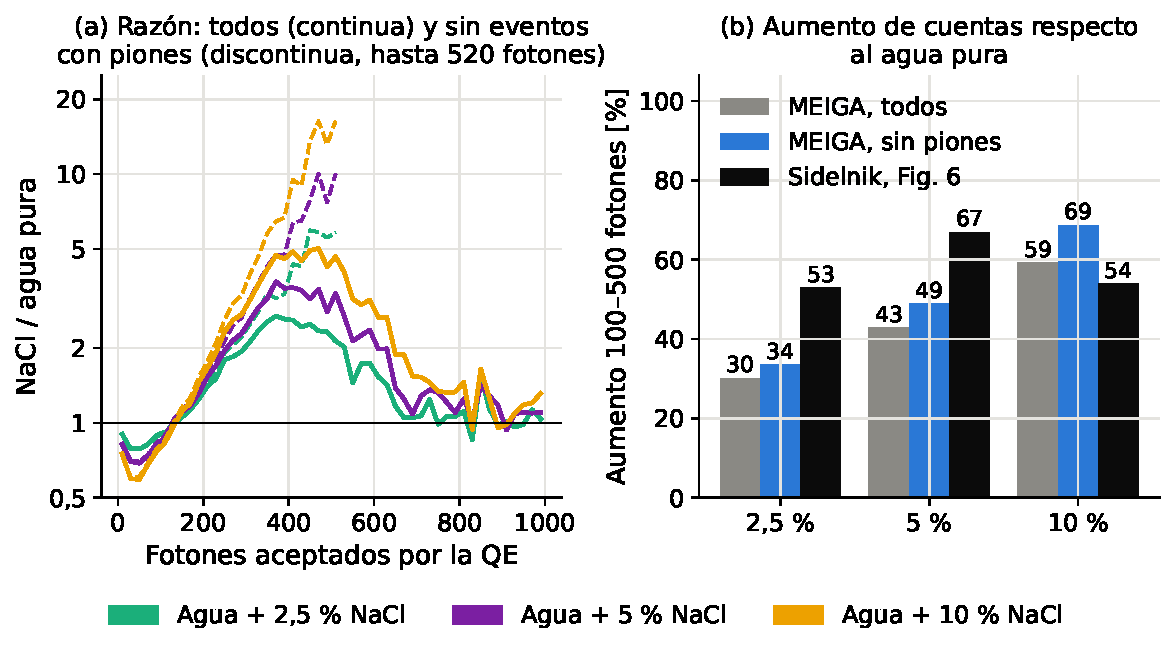
\includegraphics[width=\linewidth]{../figuras/fig24_piones_efecto_nacl.pdf}\caption{Efecto del NaCl en la Fig.~6 con y sin los eventos con producción de piones: (a) razón NaCl/agua pura de los fotones aceptados; (b) aumento de cuentas entre 100 y 500 fotones respecto al agua pura, MEIGA (todos los eventos y sin piones) frente a Sidelnik.}\end{figure}

\section{Validación cuantitativa de los histogramas de carga}
{\small\textit{Corresponde a la Sec.~4.1.1.7 de la tesis (Figs. 4.8--4.11, Tabla 4.3).}}

\subsection{Curvas de razón NaCl / agua pura (validación cuantitativa)}\label{sec:razon}
Para cuantificar el efecto del NaCl se dividió el histograma de fotones aceptados de cada medio con sal por el de agua pura, en MEIGA y en las curvas digitalizadas de la Fig.~6
(\texttt{razon\_histogramas.py}). Ambos conjuntos tienen el mismo número de neutrones por medio, de modo que se usan cuentas absolutas; los histogramas se agrupan en bines de 50 fotones
y se excluye el primero (0--50 fotones), afectado por la digitalización. Las métricas se calculan en los 19 bines entre 50 y 1000 fotones (Fig.~\ref{fig:razon}).
\begin{table}[H]\centering\small\begin{adjustbox}{max width=\linewidth}\begin{tabular}{lcccccc}\toprule
NaCl & Pearson $r$ & $p$ & Spearman $\rho$ & RMSE & MAE & Razón media 100--500 (MEIGA / Sidelnik) \\\midrule
2,5\,\% & 0,881 & 6,2$\times10^{-7}$ & 0,863 & 0,276 & 0,234 & 1,92 / 1,93 \\
5\,\% & 0,906 & 9,1$\times10^{-8}$ & 0,867 & 0,383 & 0,325 & 2,36 / 2,37 \\
10\,\% & 0,895 & 2,2$\times10^{-7}$ & 0,930 & 0,857 & 0,569 & 3,02 / 2,39 \\
\bottomrule\end{tabular}\end{adjustbox}
\caption{Concordancia entre las curvas de razón NaCl / agua pura de MEIGA y de la Fig.~6 de Sidelnik digitalizada.}\label{tab:razon}\end{table}
Las curvas de los dos trabajos tienen la misma forma: la razón es menor que 1 por debajo de $\approx$\,150 fotones (la captura en Cl desplaza eventos hacia más luz), crece hasta un máximo
(MEIGA: 2,72 en 375 fotones, 3,58 en 375 fotones, 4,74 en 475 fotones; Sidelnik: 2,44 en 325, 3,17 en 375, 4,16 en 425)
y tiende a 1 por encima de $\approx$\,700 fotones, donde dominan los piones. La razón de MEIGA crece de forma monótona con la concentración; en la figura digitalizada, en cambio,
la razón media entre 100 y 500 fotones con 10\,\% es prácticamente igual a la de 5\,\%, aunque su máximo es mayor.
El máximo de MEIGA es algo más alto y está desplazado 0--50 fotones hacia más luz, coherente con el exceso de energía de las cascadas del Cl (Sec.~\ref{sec:cascadas_cl}).
\begin{figure}[H]\centering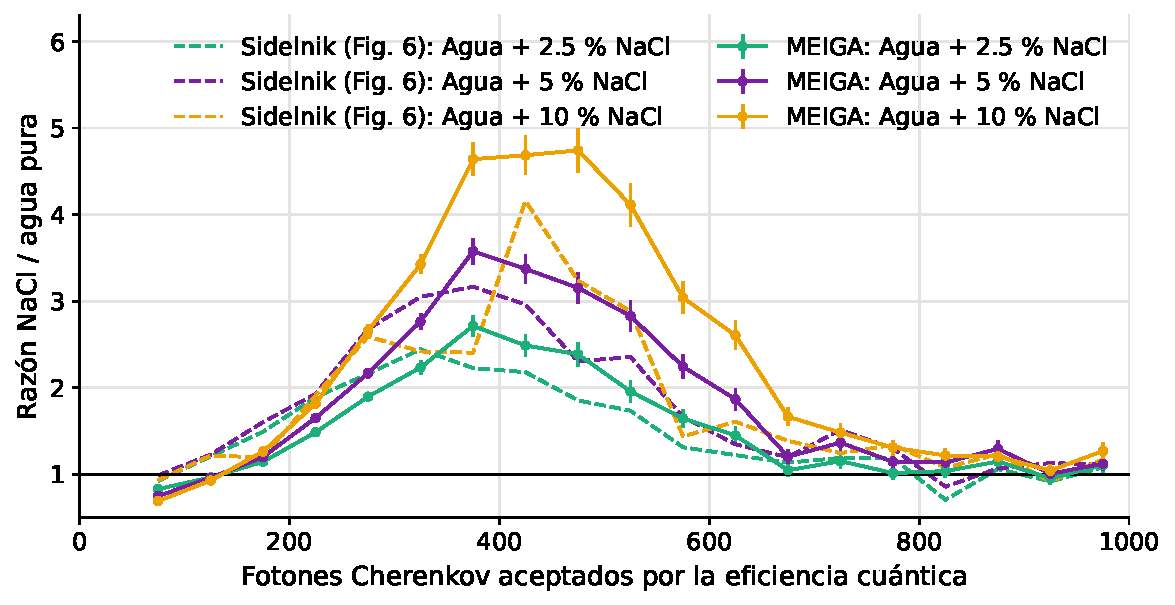
\includegraphics[width=\linewidth]{../figuras/fig22_razon_histogramas.pdf}\caption{Razón entre los histogramas de fotones aceptados de cada medio con NaCl y el de agua pura: MEIGA (puntos con error estadístico) y Fig.~6 de Sidelnik digitalizada (líneas discontinuas), bines de 50 fotones.}\label{fig:razon}\end{figure}
\subsection{Aporte: el histograma de carga en el PMT}
El eje de la Fig.~6 del artículo corresponde a los fotones Cherenkov aceptados por la eficiencia cuántica. Su escala y su forma coinciden con los fotones aceptados al crearse, antes del transporte óptico, y no con la carga en el PMT, unas 16 veces menor: la figura no parece incluir la colección óptica, aunque el artículo no lo especifica (Sec.~\ref{sec:diag}). La magnitud que mide el detector es la carga en el PMT,
que incluye el transporte de cada fotón por el agua y sus reflexiones en el Tyvek hasta llegar al fotocátodo (Sec.~\ref{sec:diag}).
Ese histograma es el aporte de este trabajo (Fig.~\ref{fig:fig09}, paneles c y d):
\begin{itemize}
\item El 53,0\,\% de los neutrones deja al menos un fotoelectrón; la mediana es 1\,p.e. y la media 9,8\,p.e. (19,5\,p.e. contando solo los eventos con carga).
\item Solo el 2,5\,\% de los eventos supera 100\,p.e. Como llega al PMT alrededor del 6\,\% de los fotones transportados, la distribución se comprime hacia valores bajos y desaparece la cola de cientos de fotones.
\end{itemize}
\aviso{La escala del histograma de carga depende del modelo óptico del Tyvek y de la longitud de absorción del agua: con la reflectividad de LHAASO (0,985) y una longitud de absorción de 100\,m,
la carga media subiría hasta unas 2,5 veces. El histograma de fotones aceptados (comparación con la Fig.~6) no depende del transporte óptico y no cambia.
La carga debe tomarse como definitiva solo después de fijar el modelo del Tyvek.}
\begin{figure}[H]\centering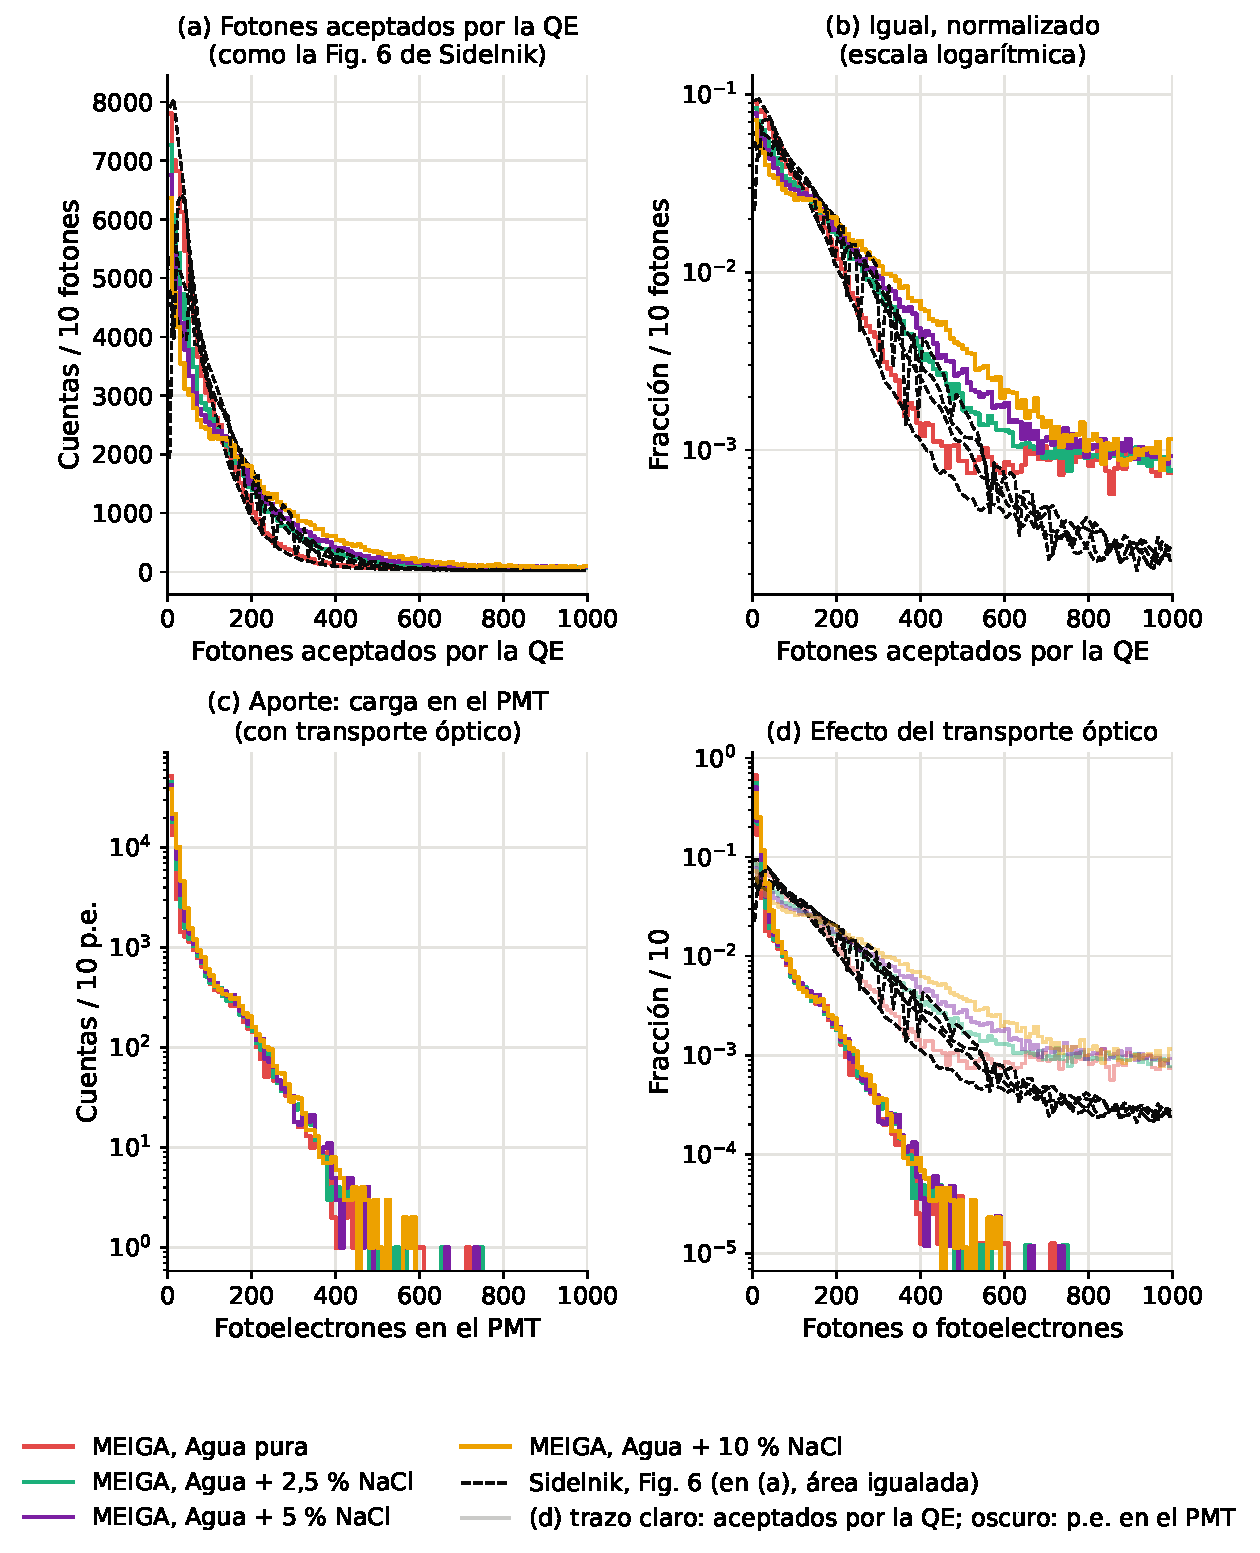
\includegraphics[width=\linewidth]{../figuras/fig09_histograma_tipo_sidelnik.pdf}\caption{(a, b) Fotones aceptados por la eficiencia cuántica antes del transporte óptico, frente a la Fig.~6 de Sidelnik (área igualada y normalizado en escala logarítmica).
(c) Histograma de carga en el PMT, con transporte óptico. (d) Efecto del transporte óptico: fotones aceptados frente a fotoelectrones. Eventos con al menos un fotón o fotoelectrón.}\label{fig:fig09}\end{figure}
\subsection{Diagnóstico: por qué la carga es baja (agua pura)}\label{sec:diag}
Se reconstruyó la historia de los 23,3 millones de fotones ópticos seguidos (archivo \texttt{pasos-particulas.tsv}, 78\,GB).
En el modo rápido de MEIGA (\texttt{eFast}) cada fotón Cherenkov se acepta o descarta según la eficiencia cuántica del R5912 en el momento de crearse;
solo los aceptados se transportan, y cada uno que entra al PMT es un fotoelectrón.
\begin{table}[H]\centering\small\begin{adjustbox}{max width=\linewidth}\begin{tabular}{lr}\toprule
Etapa & Por neutrón \\\midrule
Fotones Cherenkov creados & 1\,440,7 \\
Aceptados por la eficiencia cuántica al crearse (se transportan) & 155,6 (10,8\,\%) \\
Llegan al PMT = carga & 9,81 (6,3\,\% de los transportados) \\\bottomrule
\end{tabular}\end{adjustbox}\caption{Balance de luz. La carga registrada coincide con los fotones que entran al PMT en el 99,88\,\% de los eventos.}\end{table}
\begin{table}[H]\centering\small\begin{adjustbox}{max width=\linewidth}\begin{tabular}{lccc}\toprule
Destino del fotón transportado & Fracción & Rebotes medios & Camino medio [cm] \\\midrule
Llega al PMT & 6,3\,\% & 7,9 & 601 \\
Absorbido en el agua & 16,4\,\% & 7,3 & 539 \\
Absorbido al chocar con la pared (Tyvek) & 76,7\,\% & 7,0 & 539 \\
Perdido dentro del Tyvek/acero & 0,6\,\% & 7,3 & 560 \\
\bottomrule\end{tabular}\end{adjustbox}\caption{Destino de los fotones transportados.}\end{table}
Los pasos de fotones ``dentro del Tyvek'' son de longitud cero: son las reflexiones en la superficie \texttt{groundbackpainted}, que funciona.
La pérdida dominante es la absorción en la pared. Con un modelo de rebotes ajustado a las trayectorias (\texttt{sensibilidad\_tyvek.py}): en cada encuentro con la pared el fotón alcanza el PMT con probabilidad $s$, si no choca con el Tyvek y se absorbe con probabilidad $a$, y entre encuentros se absorbe en el agua con probabilidad $w$; la fracción que llega al PMT es $P = s/[s + (1-s)a + w]$.
En agua pura $s = 0{,}8$\,\%, $a = 9{,}8$\,\% y $w = 2{,}0$\,\%, que dan $P = 6{,}3$\,\%, igual al valor observado: un fotón sobrevive en promedio $1/a \approx 10$ choques, pero necesitaría del orden de $1/s \approx 130$ encuentros para dar con el PMT.
\paragraph{El factor 0,94 del Tyvek.} En \texttt{Materials.cc} la reflectividad medida del Tyvek ($R_{\rm tabla}$: 0,99--1,00 en el azul, 0,78--0,85 en el ultravioleta) se multiplica por \texttt{scaleLinerRef}\,=\,0,94. De los 9,8 puntos de absorción por choque, $\approx$\,2,1 corresponden a $1 - R_{\rm tabla}$, $\approx$\,5,9 al factor 0,94 (una pérdida mínima del 6\,\% por choque aun donde el Tyvek tabulado refleja el 100\,\%) y $\approx$\,1,9 a una pérdida adicional del modelo de superficie \texttt{groundbackpainted}.
El factor es un parámetro del modelo sin justificación documentada (se usa a veces para representar un revestimiento envejecido) y es el principal responsable de la baja colección. Carga media estimada con otros modelos ópticos (agua pura):
\begin{table}[H]\centering\small\begin{adjustbox}{max width=\linewidth}\begin{tabular}{lcc}\toprule
Modelo óptico & Carga media [p.e.] & Factor \\\midrule
Actual: $R = 0{,}94\,R_{\rm tabla}$ & 9,8 & 1,0 \\
Tabla sin el factor 0,94 & 20,9 & 2,1 \\
$R = 0{,}985$ (LHAASO) & 19,8 & 2,0 \\
Actual + agua de 100\,m & 11,0 & 1,1 \\
$R = 0{,}985$ + agua de 100\,m & 25,2 & 2,6 \\
\bottomrule\end{tabular}\end{adjustbox}\caption{Sensibilidad de la carga en el PMT al modelo óptico (modelo de rebotes aplicado por intervalos de energía del fotón; se conserva la pérdida adicional de \texttt{groundbackpainted}).}\label{tab:sens_tyvek}\end{table}
La escala absoluta de la carga es incierta en un factor de hasta $\approx$\,2,5, pero ni la comparación con la Fig.~6 (fotones aceptados antes del transporte) ni las diferencias entre medios dependen de ella. El Tyvek se mantuvo en esta campaña para que todas las corridas sean comparables; su revisión queda como trabajo futuro.
La luz roja ($<2{,}3$\,eV) se pierde sobre todo por absorción en el agua (longitud de absorción de 3--9\,m), y la ultravioleta por la menor reflectividad del Tyvek.
\begin{figure}[H]\centering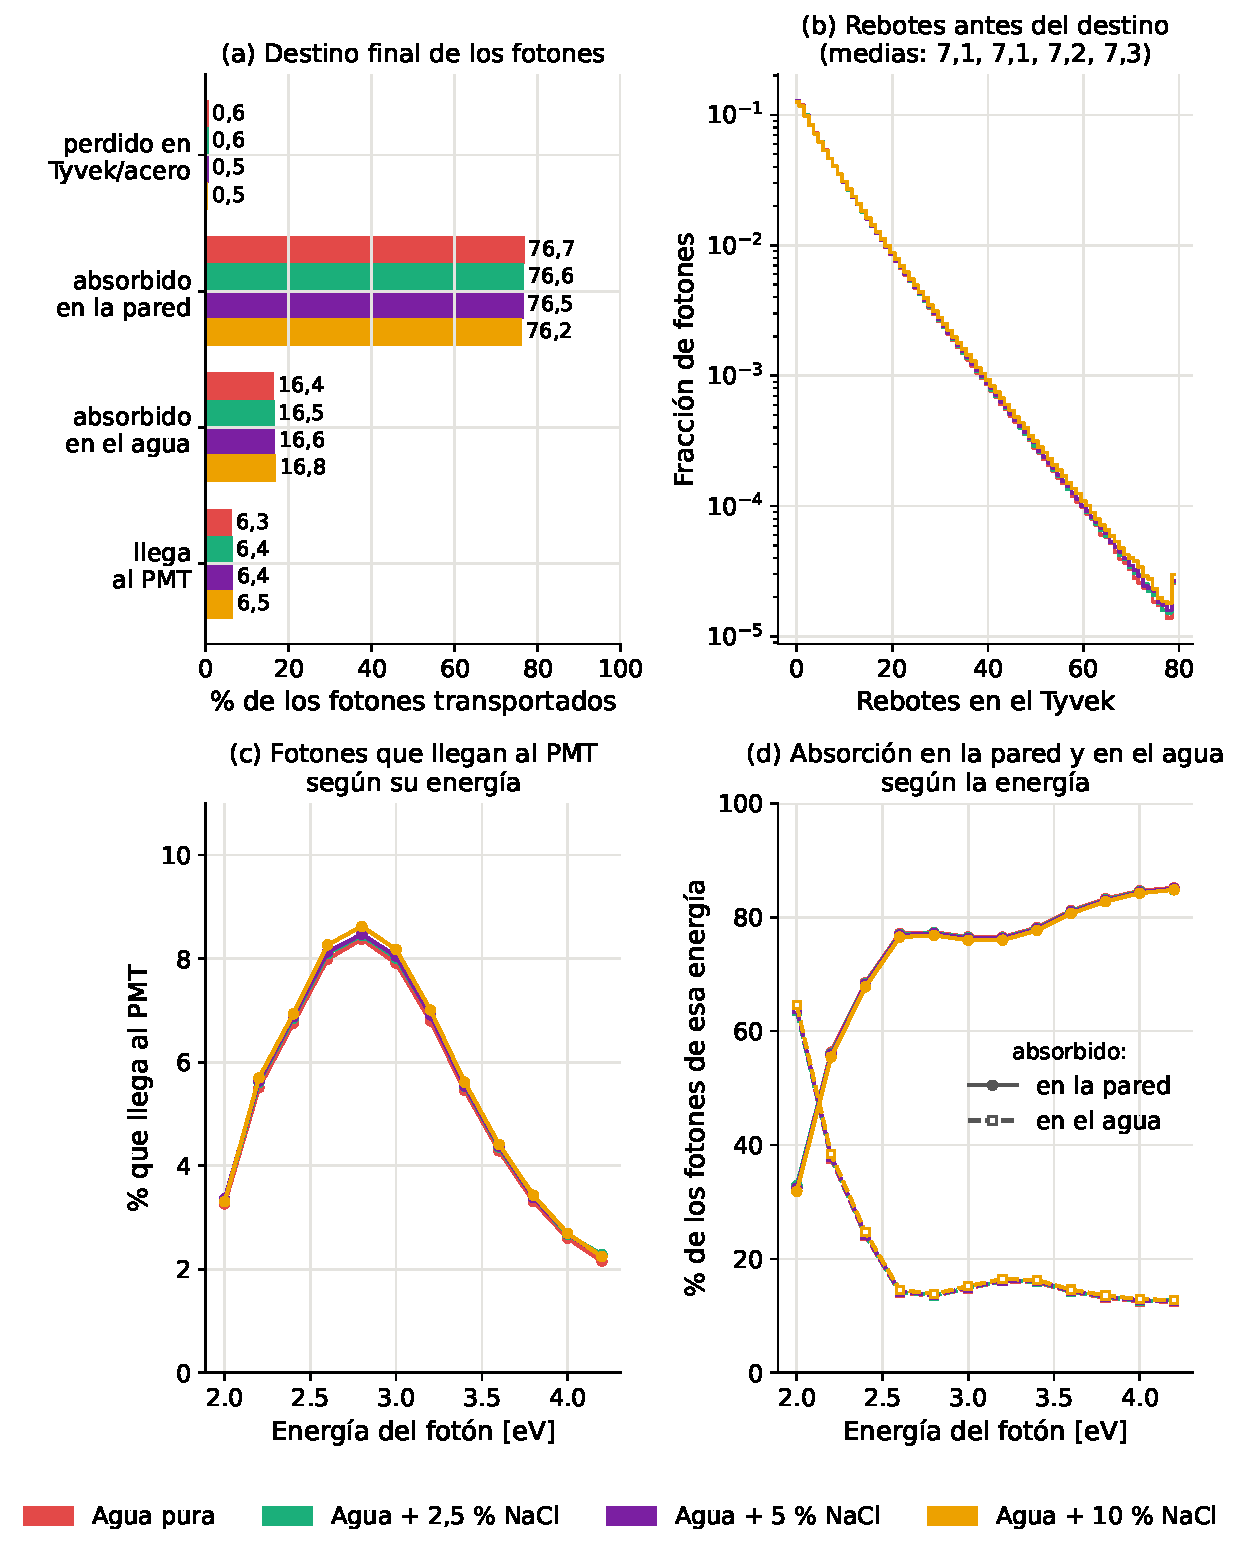
\includegraphics[width=\linewidth]{../figuras/fig07_destino_fotones.pdf}\caption{Destino de los fotones transportados en los cuatro medios (\texttt{figura\_destino\_fotones\_medios.py}): (a) destino final; (b) rebotes en el Tyvek antes del destino; (c) fracción que llega al PMT según la energía del fotón; (d) fracción absorbida en la pared y en el agua según la energía.}\label{fig:destino}\end{figure}
\paragraph{Qué cuenta la Fig. 6 de Sidelnik.} Su eje dice ``número de fotones Cherenkov aceptados por la eficiencia cuántica''. La distribución de MEIGA que mejor
la reproduce es precisamente la de fotones aceptados por la eficiencia cuántica al crearse, antes del transporte óptico (correlación de la forma en escala logarítmica 0,966,
frente a 0,878 para la carga en el PMT), incluido el quiebre a 400--450 fotones.
Esto indica que la Fig.~6 del artículo no incluye la eficiencia de colección óptica, aunque el artículo no lo especifica: la carga en el PMT de MEIGA es del orden de 16 veces menor, y ni con la reflectividad de LHAASO (0,985) y 100\,m de longitud de absorción subiría más de unas 2,5 veces.
\begin{figure}[H]\centering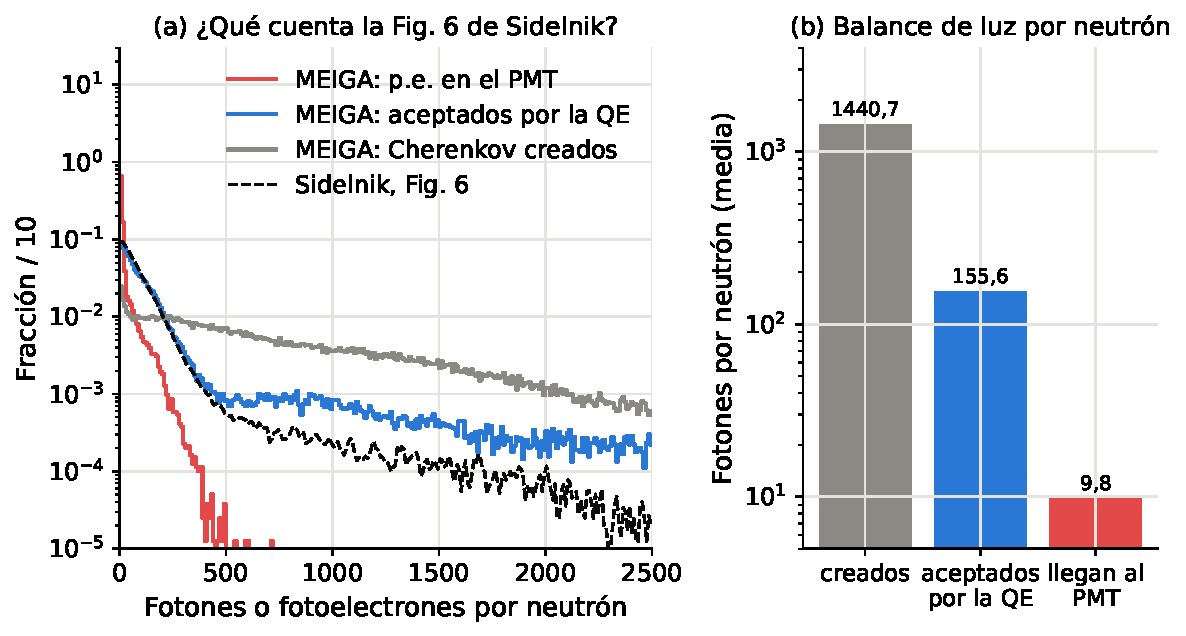
\includegraphics[width=\linewidth]{../figuras/fig06_balance_luz_y_fig6.pdf}\caption{Izquierda: tres distribuciones de MEIGA frente a la Fig.~6 de Sidelnik. Derecha: balance de luz por neutrón.}\end{figure}
\subsection{Óptica: mismo transporte en todos los medios y decisión sobre el Tyvek}
El transporte óptico es prácticamente el mismo en los cuatro medios (Fig.~\ref{fig:destino}): llega al PMT el 6,30, 6,39, 6,41 y 6,50\,\% de los fotones transportados (agua pura, 2,5, 5 y 10\,\% NaCl), se absorbe en la pared el 76,7--76,2\,\% y en el agua el 16,4--16,8\,\%, con 7,1--7,3 rebotes medios; la dependencia con la energía del fotón es idéntica. En detalle, llega al PMT el 6,30\,\% (agua pura) y el 6,39\,\% (2,5\,\% NaCl) de los fotones transportados,
y la probabilidad de absorción por choque con la pared es 9,75\,\% y 9,69\,\%. La razón carga/fotón creado no cambia
(0,679 y 0,685\,\%). Por tanto el modelo del Tyvek fija una escala común de la carga, pero no altera las diferencias entre medios:
el aumento de carga con el NaCl (+16,4\,\%) se debe solo a la mayor producción de luz.
Con el esquema actual las comparaciones con Sidelnik (captura, espectros, Fig.~6 con su mismo observable) y la comparación relativa de la carga entre medios son válidas.
Mantener el Tyvek actual en las corridas de 2,5, 5 y 10\,\% NaCl asegura que los cuatro medios sean comparables con la corrida de agua pura; un Tyvek corregido obligaría a repetir también el agua pura.
\section{Conclusiones preliminares}
\begin{enumerate}
\item La configuración de la corrida es la del artículo: los 150\,000 neutrones parten de $(-49{,}062;\,0;\,66{,}562)$\,cm con 500\,MeV, y la prueba de 10 neutrones verificó materiales, espesores, posición del PMT y física sin $S(\alpha,\beta)$.
\item La física de captura es coherente: 99,94\,\% de las capturas en H, $\tau = 192$\,µs (teórico $\approx$\,200\,µs para agua pura con H libre) y espectros con las líneas y bordes Compton esperados.
\item La probabilidad de captura de la Tabla~2 de Sidelnik se reproduce si se interpreta como capturas en el agua divididas por todos los neutrones del evento (primario + cascada): 24,08\,\% frente a 25,18\,\% en agua pura. La captura de la traza primaria (0,88\,\%) no es comparable. La distancia de máxima absorción
solo coincide en escala si se mide desde el vértice del neutrón capturado.
\item La carga en el PMT es baja por la óptica del detector: el 77\,\% de los fotones se absorbe en la pared de Tyvek y solo el 6\,\% llega al PMT. La Fig.~6 de Sidelnik coincide con los fotones aceptados por la eficiencia cuántica antes del transporte, no con la carga del PMT.
\item El espectro gamma reproduce la Fig.~3 de Sidelnik en las líneas de 2,223 y 6,13\,MeV (cociente 0,022 en ambos, sin el $^{16}$N) y en el continuo de 2,5--9\,MeV; la línea de 0,511\,MeV es unas 6 veces más intensa por los emisores $\beta^+$ de larga vida y la producción de piones (Sec.~\ref{sec:fig3}).
\item Con el observable de Sidelnik (Sec.~\ref{sec:fig6}), MEIGA reproduce su Fig.~6 entre 0 y 500 fotones en forma y en cuentas absolutas, sin reescalar. Por encima de 500 fotones MEIGA tiene 2--3 veces más eventos; esa cola se debe casi por completo a eventos con producción de piones, probablemente por diferencias en el modelo hadrónico a 500\,MeV.
\item Medios con NaCl (2,5, 5 y 10\,\%, 150\,000 neutrones cada uno; Secs.~\ref{sec:nacl25} y \ref{sec:razon}): las tendencias con la sal tienen el signo de Sidelnik y son monótonas (más capturas, menor distancia, $\tau$ de 192 a 140, 109, 75\,µs, como predicen las secciones eficaces térmicas; luz adicional entre 150 y 550 fotones en la Fig.~6), aunque el aumento de la fracción de captura es unas dos veces menor que en el artículo. Las curvas de razón NaCl/agua pura de la Fig.~6 coinciden con las del artículo ($r \geq 0{,}88$). Las líneas del Cl de 1,165--7,79\,MeV coinciden con el artículo; las cascadas del $^{35}$Cl de Geant4 no conservan la energía (exceso de la línea de 8,58\,MeV); el transporte óptico es idéntico en todos los medios, por lo que el Tyvek no afecta a la comparación entre medios.
\item El espectro de electrones producidos por gammas reproduce la Fig.~5 de Sidelnik en escala absoluta (bines de 20\,keV, cociente $\approx$\,1,06) y en forma, incluidos los bordes Compton y el aumento con NaCl entre 2 y 6\,MeV; solo el borde de 8,33\,MeV difiere, por las cascadas del $^{35}$Cl (Sec.~\ref{sec:fig5}).
\item Las diferencias con la Fig.~5 tienen una explicación física (Sec.~\ref{sec:interp_fig5}): por cada captura en H, MEIGA produce $\approx$\,1,6 veces más gammas de desexcitación nuclear tras la dispersión inelástica de neutrones, lo que reduce el salto en el borde de 1,994\,MeV y diluye el efecto del NaCl entre 2 y 6\,MeV; el exceso entre 7 y 8,3\,MeV se debe a las cascadas del $^{35}$Cl.
\item El aporte nuevo es el histograma de carga en el PMT, que incluye el transporte óptico. Su escala absoluta depende del modelo del Tyvek; las diferencias entre medios no.
\end{enumerate}
\appendix
\section{Ecuaciones, energías y porcentajes de todos los procesos}\label{sec:procesos}
Las Tablas~\ref{tab:procesos_pura}--\ref{tab:procesos_nacl10} reúnen, para cada medio, todas las reacciones de los neutrones en el volumen del detector (primario y secundarios): la ecuación,
el valor $Q$ del estado fundamental (calculado con los excesos de masa AME2020; $Q<0$ es la energía umbral que se gasta en romper el núcleo), la energía típica del neutrón incidente,
el porcentaje dentro de cada tipo de proceso y los gammas que emite (\texttt{canales\_reaccion.py}; el blanco de cada inelástica se deduce por conservación de la carga y del número bariónico).
En las inelásticas, las \emph{líneas} solo se atribuyen si pertenecen al núcleo residual o al blanco de esa misma reacción (ventana de $\pm10$\,keV).
{\footnotesize\begin{longtable}{p{4.4cm}rrrp{4.6cm}}
\caption{Agua pura: ecuaciones, energías y porcentajes de los procesos de los neutrones (150\,000 neutrones de 500\,MeV).}\label{tab:procesos_pura}\\\toprule
Reacción & $Q$ [MeV] & $E_n$ típica & \% & Gammas / resultado (keV) \\\midrule\endfirsthead
\toprule Reacción & $Q$ [MeV] & $E_n$ típica & \% & Gammas / resultado (keV) \\\midrule\endhead
\multicolumn{5}{l}{\textbf{Dispersión elástica} (104 por neutrón incidente; \% de las colisiones con blanco reconstruido, $E>1$\,eV)}\\
$^1$H(n,n)$^1$H & 0 & todas & 83,74\,\% & pierde 0--100\,\% de $E$; $\xi = 1{,}00$ \\
$^{16}$O(n,n)$^{16}$O & 0 & todas & 15,95\,\% & pierde 0--22\,\%; $\xi = 0{,}12$ ($<$\,1\,MeV) \\
\midrule\multicolumn{5}{l}{\textbf{Captura radiativa} (0,829 por neutrón incidente; \% de las capturas en el agua)}\\
$^1$H(n,$\gamma$)$^2$H & +2,225 & térmica & 99,94\,\% & 2224 (MEIGA: 2224,4) \\
$^{16}$O(n,$\gamma$)$^{17}$O & +4,143 & térmica & 0,06\,\% & 871, 1088, 2184; $\gamma$ único 4143 \\
\midrule\multicolumn{5}{l}{\textbf{Inelástica} (1,29 por neutrón incidente; \% de las inelásticas; canales con más del 0,4\,\%)}\\
$^{16}$O(n,np)$^{15}$N & -12,13 & 354\,MeV & 12,9\,\% & 2,2 $\gamma$/reacc.; continuo \\
$^{16}$O(n,n')$^{16}$O & 0,00 & 21\,MeV (48\,\% $<$\,20) & 11,3\,\% & 2,8 $\gamma$/reacc.; 6130 (14\,\%), 7117 (6\,\%), 2741 (4\,\%) \\
$^{16}$O(n,n$\alpha$)$^{12}$C & -7,16 & 39\,MeV (16\,\% $<$\,20) & 9,5\,\% & 1,7 $\gamma$/reacc.; 4439 (6\,\%) \\
$^{16}$O(n,2n)$^{15}$O & -15,66 & 500\,MeV & 9,4\,\% & 2,1 $\gamma$/reacc.; continuo \\
$^{16}$O(n,2np)$^{14}$N & -22,96 & 377\,MeV & 9,1\,\% & 2,0 $\gamma$/reacc.; continuo \\
$^{16}$O(n,3n2p)$^{12}$C & -35,46 & 500\,MeV & 6,7\,\% & 2,1 $\gamma$/reacc.; continuo \\
$^{16}$O(n,2n2p)$^{13}$C & -30,51 & 477\,MeV & 4,0\,\% & 1,7 $\gamma$/reacc.; continuo \\
$^{16}$O(n,$\alpha$)$^{13}$C & -2,22 & 10\,MeV (100\,\% $<$\,20) & 3,1\,\% & 2,4 $\gamma$/reacc.; continuo \\
$^{16}$O(n,n2p)$^{14}$C & -22,33 & 384\,MeV & 2,9\,\% & 2,1 $\gamma$/reacc.; continuo \\
$^{16}$O(n,3n2p$\alpha$)$^{8}$Be & -42,82 & 500\,MeV & 2,1\,\% & 1,6 $\gamma$/reacc.; continuo \\
$^{16}$O(n,2npd)$^{12}$C & -33,23 & 380\,MeV & 1,9\,\% & 2,2 $\gamma$/reacc.; continuo \\
$^{16}$O(n,3n2p3$\alpha$) & -42,73 & 500\,MeV & 1,4\,\% & 1,7 $\gamma$/reacc.; continuo \\
$^{16}$O(n,3np)$^{13}$N & -33,51 & 500\,MeV & 1,1\,\% & 1,6 $\gamma$/reacc.; continuo \\
$^{16}$O(n,n2$\alpha$)$^{8}$Be & -14,53 & 68\,MeV & 1,0\,\% & 1,5 $\gamma$/reacc.; continuo \\
$^{16}$O(n,3n3p)$^{11}$B & -51,41 & 500\,MeV & 0,8\,\% & 2,3 $\gamma$/reacc.; continuo \\
$^{16}$O(n,np$\pi^-$)$^{15}$O & -154,45 & 500\,MeV & 0,7\,\% & 2,3 $\gamma$/reacc.; continuo \\
$^{16}$O(n,p)$^{16}$N & -9,64 & 19\,MeV (54\,\% $<$\,20) & 0,7\,\% & 2,0 $\gamma$/reacc.; continuo \\
$^{1}$H(n,np$\pi^0$) & -134,98 & 500\,MeV & 0,7\,\% & 0,0 $\gamma$/reacc.; sin $\gamma$ directos \\
$^{16}$O(n,2npd$\alpha$)$^{8}$Be & -40,60 & 500\,MeV & 0,7\,\% & 1,6 $\gamma$/reacc.; continuo \\
$^{16}$O(n,3n)$^{14}$O & -28,89 & 500\,MeV & 0,7\,\% & 2,1 $\gamma$/reacc.; continuo \\
$^{16}$O(n,np$\pi^0$)$^{15}$N & -147,10 & 500\,MeV & 0,6\,\% & 2,6 $\gamma$/reacc.; continuo \\
$^{16}$O(n,4n3pd2$\alpha$) & -68,80 & 500\,MeV & 0,5\,\% & 2,0 $\gamma$/reacc.; continuo \\
$^{16}$O(n,4n3p)$^{10}$B & -62,87 & 500\,MeV & 0,5\,\% & 1,8 $\gamma$/reacc.; continuo \\
$^{16}$O(n,5n4p2$\alpha$) & -71,03 & 500\,MeV & 0,5\,\% & 1,9 $\gamma$/reacc.; continuo \\
$^{16}$O(n,2n3p$\pi^-$)$^{12}$C & -174,25 & 500\,MeV & 0,5\,\% & 2,1 $\gamma$/reacc.; continuo \\
$^{16}$O(n,4n2p)$^{11}$C & -54,18 & 500\,MeV & 0,5\,\% & 2,2 $\gamma$/reacc.; continuo \\
$^{16}$O(n,n2p$\pi^-$)$^{14}$N & -161,75 & 500\,MeV & 0,4\,\% & 2,0 $\gamma$/reacc.; continuo \\
$^{16}$O(n,2npd3$\alpha$) & -40,51 & 500\,MeV & 0,4\,\% & 1,6 $\gamma$/reacc.; continuo \\
$^{16}$O(n,3n2p$\pi^0$)$^{12}$C & -170,43 & 500\,MeV & 0,4\,\% & 2,2 $\gamma$/reacc.; continuo \\
\bottomrule\end{longtable}}
{\footnotesize\begin{longtable}{p{4.4cm}rrrp{4.6cm}}
\caption{2,5\,\% NaCl: ecuaciones, energías y porcentajes de los procesos de los neutrones (150\,000 neutrones de 500\,MeV).}\label{tab:procesos_nacl25}\\\toprule
Reacción & $Q$ [MeV] & $E_n$ típica & \% & Gammas / resultado (keV) \\\midrule\endfirsthead
\toprule Reacción & $Q$ [MeV] & $E_n$ típica & \% & Gammas / resultado (keV) \\\midrule\endhead
\multicolumn{5}{l}{\textbf{Dispersión elástica} (83 por neutrón incidente; \% de las colisiones con blanco reconstruido, $E>1$\,eV)}\\
$^1$H(n,n)$^1$H & 0 & todas & 83,55\,\% & pierde 0--100\,\% de $E$; $\xi = 1{,}00$ \\
$^{16}$O(n,n)$^{16}$O & 0 & todas & 15,82\,\% & pierde 0--22\,\%; $\xi = 0{,}12$ ($<$\,1\,MeV) \\
$^{23}$Na(n,n)$^{23}$Na & 0 & todas & 0,47\,\% & pierde 0--16\,\% \\
$^{35,37}$Cl(n,n)$^{35,37}$Cl & 0 & todas & 0,16\,\% & pierde 0--11\,\% \\
\midrule\multicolumn{5}{l}{\textbf{Captura radiativa} (0,864 por neutrón incidente; \% de las capturas en el agua)}\\
$^1$H(n,$\gamma$)$^2$H & +2,225 & térmica & 63,53\,\% & 2224 (MEIGA: 2224,4) \\
$^{35}$Cl(n,$\gamma$)$^{36}$Cl & +8,580 & térmica & 35,75\,\% & 517, 788, 1165, 1951, 6111, 7414; $\gamma$ único 8580 \\
$^{23}$Na(n,$\gamma$)$^{24}$Na & +6,959 & térmica & 0,57\,\% & 472 (0,9\,\%); $\gamma$ único 6959 \\
$^{37}$Cl(n,$\gamma$)$^{38}$Cl & +6,108 & térmica & 0,11\,\% & 638, 755, 1692; $\gamma$ único 6108 \\
$^{16}$O(n,$\gamma$)$^{17}$O & +4,143 & térmica & 0,03\,\% & 871, 1088, 2184; $\gamma$ único 4143 \\
\midrule\multicolumn{5}{l}{\textbf{Inelástica} (1,33 por neutrón incidente; \% de las inelásticas; canales con más del 0,4\,\% y los del Na y el Cl)}\\
$^{16}$O(n,np)$^{15}$N & -12,13 & 350\,MeV & 12,6\,\% & 2,2 $\gamma$/reacc.; continuo \\
$^{16}$O(n,n')$^{16}$O & 0,00 & 21\,MeV (49\,\% $<$\,20) & 11,0\,\% & 2,8 $\gamma$/reacc.; 6130 (14\,\%), 7117 (6\,\%), 6917 (4\,\%) \\
$^{16}$O(n,n$\alpha$)$^{12}$C & -7,16 & 39\,MeV (16\,\% $<$\,20) & 9,3\,\% & 1,7 $\gamma$/reacc.; 4439 (6\,\%) \\
$^{16}$O(n,2n)$^{15}$O & -15,66 & 500\,MeV & 9,0\,\% & 2,1 $\gamma$/reacc.; continuo \\
$^{16}$O(n,2np)$^{14}$N & -22,96 & 373\,MeV & 8,8\,\% & 2,0 $\gamma$/reacc.; continuo \\
$^{16}$O(n,3n2p)$^{12}$C & -35,46 & 500\,MeV & 6,4\,\% & 2,1 $\gamma$/reacc.; continuo \\
$^{16}$O(n,2n2p)$^{13}$C & -30,51 & 471\,MeV & 4,0\,\% & 1,7 $\gamma$/reacc.; continuo \\
$^{16}$O(n,$\alpha$)$^{13}$C & -2,22 & 10\,MeV (100\,\% $<$\,20) & 3,1\,\% & 2,4 $\gamma$/reacc.; continuo \\
$^{16}$O(n,n2p)$^{14}$C & -22,33 & 406\,MeV & 2,8\,\% & 2,0 $\gamma$/reacc.; continuo \\
$^{16}$O(n,3n2p$\alpha$)$^{8}$Be & -42,82 & 500\,MeV & 2,0\,\% & 1,6 $\gamma$/reacc.; continuo \\
$^{16}$O(n,2npd)$^{12}$C & -33,23 & 399\,MeV & 1,8\,\% & 2,2 $\gamma$/reacc.; continuo \\
$^{16}$O(n,3n2p3$\alpha$) & -42,73 & 500\,MeV & 1,5\,\% & 1,7 $\gamma$/reacc.; continuo \\
$^{16}$O(n,3np)$^{13}$N & -33,51 & 500\,MeV & 1,1\,\% & 1,7 $\gamma$/reacc.; continuo \\
$^{16}$O(n,n2$\alpha$)$^{8}$Be & -14,53 & 70\,MeV & 1,0\,\% & 1,5 $\gamma$/reacc.; continuo \\
$^{16}$O(n,3n3p)$^{11}$B & -51,41 & 500\,MeV & 0,8\,\% & 2,3 $\gamma$/reacc.; continuo \\
$^{16}$O(n,np$\pi^-$)$^{15}$O & -154,45 & 500\,MeV & 0,7\,\% & 2,3 $\gamma$/reacc.; continuo \\
$^{16}$O(n,p)$^{16}$N & -9,64 & 19\,MeV (54\,\% $<$\,20) & 0,7\,\% & 2,0 $\gamma$/reacc.; continuo \\
$^{16}$O(n,3n)$^{14}$O & -28,89 & 500\,MeV & 0,6\,\% & 2,2 $\gamma$/reacc.; continuo \\
$^{1}$H(n,np$\pi^0$) & -134,98 & 500\,MeV & 0,6\,\% & 0,0 $\gamma$/reacc.; sin $\gamma$ directos \\
$^{16}$O(n,2npd$\alpha$)$^{8}$Be & -40,60 & 472\,MeV & 0,6\,\% & 1,6 $\gamma$/reacc.; continuo \\
$^{16}$O(n,np$\pi^0$)$^{15}$N & -147,10 & 500\,MeV & 0,6\,\% & 2,7 $\gamma$/reacc.; continuo \\
$^{16}$O(n,4n3pd2$\alpha$) & -68,80 & 500\,MeV & 0,5\,\% & 1,9 $\gamma$/reacc.; continuo \\
$^{16}$O(n,4n3p)$^{10}$B & -62,87 & 500\,MeV & 0,5\,\% & 1,8 $\gamma$/reacc.; continuo \\
$^{16}$O(n,2n3p$\pi^-$)$^{12}$C & -174,25 & 500\,MeV & 0,5\,\% & 2,2 $\gamma$/reacc.; continuo \\
$^{16}$O(n,5n4p2$\alpha$) & -71,03 & 500\,MeV & 0,5\,\% & 1,9 $\gamma$/reacc.; continuo \\
$^{16}$O(n,4n2p)$^{11}$C & -54,18 & 500\,MeV & 0,5\,\% & 2,2 $\gamma$/reacc.; continuo \\
$^{16}$O(n,n2p$\pi^-$)$^{14}$N & -161,75 & 500\,MeV & 0,4\,\% & 2,0 $\gamma$/reacc.; continuo \\
$^{23}$Na(n,n')$^{23}$Na & 0,00 & 7\,MeV (85\,\% $<$\,20) & 0,3\,\% & 2,6 $\gamma$/reacc.; 440 (74\,\%) \\
$^{35}$Cl(n,p)$^{35}$S & 0,62 & térmica (96\,\% $<$\,20) & 0,3\,\% & 0,4 $\gamma$/reacc.; continuo \\
\bottomrule\end{longtable}}
{\footnotesize\begin{longtable}{p{4.4cm}rrrp{4.6cm}}
\caption{5\,\% NaCl: ecuaciones, energías y porcentajes de los procesos de los neutrones (150\,000 neutrones de 500\,MeV).}\label{tab:procesos_nacl5}\\\toprule
Reacción & $Q$ [MeV] & $E_n$ típica & \% & Gammas / resultado (keV) \\\midrule\endfirsthead
\toprule Reacción & $Q$ [MeV] & $E_n$ típica & \% & Gammas / resultado (keV) \\\midrule\endhead
\multicolumn{5}{l}{\textbf{Dispersión elástica} (72 por neutrón incidente; \% de las colisiones con blanco reconstruido, $E>1$\,eV)}\\
$^1$H(n,n)$^1$H & 0 & todas & 83,33\,\% & pierde 0--100\,\% de $E$; $\xi = 1{,}00$ \\
$^{16}$O(n,n)$^{16}$O & 0 & todas & 15,71\,\% & pierde 0--22\,\%; $\xi = 0{,}12$ ($<$\,1\,MeV) \\
$^{23}$Na(n,n)$^{23}$Na & 0 & todas & 0,68\,\% & pierde 0--16\,\% \\
$^{35,37}$Cl(n,n)$^{35,37}$Cl & 0 & todas & 0,28\,\% & pierde 0--11\,\% \\
\midrule\multicolumn{5}{l}{\textbf{Captura radiativa} (0,903 por neutrón incidente; \% de las capturas en el agua)}\\
$^{35}$Cl(n,$\gamma$)$^{36}$Cl & +8,580 & térmica & 51,47\,\% & 517, 788, 1165, 1951, 6111, 7414; $\gamma$ único 8580 \\
$^1$H(n,$\gamma$)$^2$H & +2,225 & térmica & 47,53\,\% & 2224 (MEIGA: 2224,4) \\
$^{23}$Na(n,$\gamma$)$^{24}$Na & +6,959 & térmica & 0,80\,\% & 472 (0,9\,\%); $\gamma$ único 6959 \\
$^{37}$Cl(n,$\gamma$)$^{38}$Cl & +6,108 & térmica & 0,17\,\% & 638, 755, 1692; $\gamma$ único 6108 \\
$^{16}$O(n,$\gamma$)$^{17}$O & +4,143 & térmica & 0,03\,\% & 871, 1088, 2184; $\gamma$ único 4143 \\
\midrule\multicolumn{5}{l}{\textbf{Inelástica} (1,36 por neutrón incidente; \% de las inelásticas; canales con más del 0,4\,\% y los del Na y el Cl)}\\
$^{16}$O(n,np)$^{15}$N & -12,13 & 326\,MeV & 12,1\,\% & 2,2 $\gamma$/reacc.; continuo \\
$^{16}$O(n,n')$^{16}$O & 0,00 & 20\,MeV (50\,\% $<$\,20) & 10,8\,\% & 2,8 $\gamma$/reacc.; 6130 (14\,\%), 7117 (6\,\%), 6917 (4\,\%) \\
$^{16}$O(n,n$\alpha$)$^{12}$C & -7,16 & 38\,MeV (16\,\% $<$\,20) & 9,2\,\% & 1,7 $\gamma$/reacc.; 4439 (6\,\%) \\
$^{16}$O(n,2n)$^{15}$O & -15,66 & 500\,MeV & 8,7\,\% & 2,1 $\gamma$/reacc.; continuo \\
$^{16}$O(n,2np)$^{14}$N & -22,96 & 352\,MeV & 8,7\,\% & 2,0 $\gamma$/reacc.; continuo \\
$^{16}$O(n,3n2p)$^{12}$C & -35,46 & 500\,MeV & 6,2\,\% & 2,1 $\gamma$/reacc.; continuo \\
$^{16}$O(n,2n2p)$^{13}$C & -30,51 & 465\,MeV & 3,8\,\% & 1,7 $\gamma$/reacc.; continuo \\
$^{16}$O(n,$\alpha$)$^{13}$C & -2,22 & 10\,MeV (100\,\% $<$\,20) & 3,0\,\% & 2,4 $\gamma$/reacc.; continuo \\
$^{16}$O(n,n2p)$^{14}$C & -22,33 & 354\,MeV & 2,7\,\% & 2,1 $\gamma$/reacc.; continuo \\
$^{16}$O(n,3n2p$\alpha$)$^{8}$Be & -42,82 & 500\,MeV & 2,0\,\% & 1,6 $\gamma$/reacc.; continuo \\
$^{16}$O(n,2npd)$^{12}$C & -33,23 & 362\,MeV & 1,8\,\% & 2,2 $\gamma$/reacc.; continuo \\
$^{16}$O(n,3n2p3$\alpha$) & -42,73 & 500\,MeV & 1,4\,\% & 1,7 $\gamma$/reacc.; continuo \\
$^{16}$O(n,3np)$^{13}$N & -33,51 & 500\,MeV & 1,1\,\% & 1,6 $\gamma$/reacc.; continuo \\
$^{16}$O(n,n2$\alpha$)$^{8}$Be & -14,53 & 71\,MeV & 1,0\,\% & 1,5 $\gamma$/reacc.; continuo \\
$^{16}$O(n,3n3p)$^{11}$B & -51,41 & 500\,MeV & 0,7\,\% & 2,3 $\gamma$/reacc.; continuo \\
$^{16}$O(n,np$\pi^-$)$^{15}$O & -154,45 & 500\,MeV & 0,6\,\% & 2,3 $\gamma$/reacc.; continuo \\
$^{16}$O(n,2npd$\alpha$)$^{8}$Be & -40,60 & 487\,MeV & 0,6\,\% & 1,6 $\gamma$/reacc.; continuo \\
$^{16}$O(n,p)$^{16}$N & -9,64 & 18\,MeV (55\,\% $<$\,20) & 0,6\,\% & 1,9 $\gamma$/reacc.; continuo \\
$^{1}$H(n,np$\pi^0$) & -134,98 & 500\,MeV & 0,6\,\% & 0,0 $\gamma$/reacc.; sin $\gamma$ directos \\
$^{16}$O(n,3n)$^{14}$O & -28,89 & 500\,MeV & 0,6\,\% & 2,1 $\gamma$/reacc.; continuo \\
$^{16}$O(n,np$\pi^0$)$^{15}$N & -147,10 & 500\,MeV & 0,5\,\% & 2,6 $\gamma$/reacc.; continuo \\
$^{23}$Na(n,n')$^{23}$Na & 0,00 & 7\,MeV (84\,\% $<$\,20) & 0,5\,\% & 2,5 $\gamma$/reacc.; 440 (72\,\%), 2076 (2\,\%) \\
$^{16}$O(n,4n3pd2$\alpha$) & -68,80 & 500\,MeV & 0,5\,\% & 1,9 $\gamma$/reacc.; continuo \\
$^{16}$O(n,4n2p)$^{11}$C & -54,18 & 500\,MeV & 0,5\,\% & 2,2 $\gamma$/reacc.; continuo \\
$^{16}$O(n,4n3p)$^{10}$B & -62,87 & 500\,MeV & 0,5\,\% & 1,8 $\gamma$/reacc.; continuo \\
$^{35}$Cl(n,p)$^{35}$S & 0,62 & térmica (96\,\% $<$\,20) & 0,5\,\% & 0,5 $\gamma$/reacc.; continuo \\
$^{16}$O(n,5n4p2$\alpha$) & -71,03 & 500\,MeV & 0,4\,\% & 1,9 $\gamma$/reacc.; continuo \\
$^{16}$O(n,2n3p$\pi^-$)$^{12}$C & -174,25 & 500\,MeV & 0,4\,\% & 2,2 $\gamma$/reacc.; continuo \\
$^{16}$O(n,n2p$\pi^-$)$^{14}$N & -161,75 & 500\,MeV & 0,4\,\% & 2,1 $\gamma$/reacc.; continuo \\
$^{23}$Na(n,np)$^{22}$Ne & -8,79 & 155\,MeV & 0,3\,\% & 2,2 $\gamma$/reacc.; continuo \\
$^{35}$Cl(n,np)$^{34}$S & -6,37 & 122\,MeV & 0,3\,\% & 2,5 $\gamma$/reacc.; continuo \\
$^{35}$Cl(n,n')$^{35}$Cl & 0,00 & 7\,MeV (77\,\% $<$\,20) & 0,3\,\% & 2,4 $\gamma$/reacc.; 1219 (18\,\%), 1763 (10\,\%) \\
$^{23}$Na(n,2np)$^{21}$Ne & -19,16 & 211\,MeV & 0,2\,\% & 2,0 $\gamma$/reacc.; 440 (3\,\%) \\
$^{35}$Cl(n,2np)$^{33}$S & -17,79 & 247\,MeV & 0,2\,\% & 2,1 $\gamma$/reacc.; continuo \\
\bottomrule\end{longtable}}
{\footnotesize\begin{longtable}{p{4.4cm}rrrp{4.6cm}}
\caption{10\,\% NaCl: ecuaciones, energías y porcentajes de los procesos de los neutrones (150\,000 neutrones de 500\,MeV).}\label{tab:procesos_nacl10}\\\toprule
Reacción & $Q$ [MeV] & $E_n$ típica & \% & Gammas / resultado (keV) \\\midrule\endfirsthead
\toprule Reacción & $Q$ [MeV] & $E_n$ típica & \% & Gammas / resultado (keV) \\\midrule\endhead
\multicolumn{5}{l}{\textbf{Dispersión elástica} (59 por neutrón incidente; \% de las colisiones con blanco reconstruido, $E>1$\,eV)}\\
$^1$H(n,n)$^1$H & 0 & todas & 82,90\,\% & pierde 0--100\,\% de $E$; $\xi = 1{,}00$ \\
$^{16}$O(n,n)$^{16}$O & 0 & todas & 15,42\,\% & pierde 0--22\,\%; $\xi = 0{,}12$ ($<$\,1\,MeV) \\
$^{23}$Na(n,n)$^{23}$Na & 0 & todas & 1,12\,\% & pierde 0--16\,\% \\
$^{35,37}$Cl(n,n)$^{35,37}$Cl & 0 & todas & 0,55\,\% & pierde 0--11\,\% \\
\midrule\multicolumn{5}{l}{\textbf{Captura radiativa} (0,972 por neutrón incidente; \% de las capturas en el agua)}\\
$^{35}$Cl(n,$\gamma$)$^{36}$Cl & +8,580 & térmica & 67,66\,\% & 517, 788, 1165, 1951, 6111, 7414; $\gamma$ único 8580 \\
$^1$H(n,$\gamma$)$^2$H & +2,225 & térmica & 30,95\,\% & 2224 (MEIGA: 2224,4) \\
$^{23}$Na(n,$\gamma$)$^{24}$Na & +6,959 & térmica & 1,13\,\% & 472 (0,9\,\%); $\gamma$ único 6959 \\
$^{37}$Cl(n,$\gamma$)$^{38}$Cl & +6,108 & térmica & 0,23\,\% & 638, 755, 1692; $\gamma$ único 6108 \\
$^{16}$O(n,$\gamma$)$^{17}$O & +4,143 & térmica & 0,02\,\% & 871, 1088, 2184; $\gamma$ único 4143 \\
\midrule\multicolumn{5}{l}{\textbf{Inelástica} (1,43 por neutrón incidente; \% de las inelásticas; canales con más del 0,4\,\% y los del Na y el Cl)}\\
$^{16}$O(n,np)$^{15}$N & -12,13 & 307\,MeV & 11,6\,\% & 2,2 $\gamma$/reacc.; continuo \\
$^{16}$O(n,n')$^{16}$O & 0,00 & 20\,MeV (50\,\% $<$\,20) & 10,5\,\% & 2,7 $\gamma$/reacc.; 6130 (15\,\%), 7117 (6\,\%), 2741 (4\,\%) \\
$^{16}$O(n,n$\alpha$)$^{12}$C & -7,16 & 37\,MeV (17\,\% $<$\,20) & 8,7\,\% & 1,7 $\gamma$/reacc.; 4439 (6\,\%) \\
$^{16}$O(n,2np)$^{14}$N & -22,96 & 343\,MeV & 8,2\,\% & 2,0 $\gamma$/reacc.; continuo \\
$^{16}$O(n,2n)$^{15}$O & -15,66 & 500\,MeV & 8,2\,\% & 2,1 $\gamma$/reacc.; continuo \\
$^{16}$O(n,3n2p)$^{12}$C & -35,46 & 500\,MeV & 5,8\,\% & 2,1 $\gamma$/reacc.; continuo \\
$^{16}$O(n,2n2p)$^{13}$C & -30,51 & 460\,MeV & 3,5\,\% & 1,7 $\gamma$/reacc.; continuo \\
$^{16}$O(n,$\alpha$)$^{13}$C & -2,22 & 10\,MeV (99\,\% $<$\,20) & 2,9\,\% & 2,4 $\gamma$/reacc.; continuo \\
$^{16}$O(n,n2p)$^{14}$C & -22,33 & 326\,MeV & 2,5\,\% & 2,1 $\gamma$/reacc.; continuo \\
$^{16}$O(n,3n2p$\alpha$)$^{8}$Be & -42,82 & 500\,MeV & 1,8\,\% & 1,6 $\gamma$/reacc.; continuo \\
$^{16}$O(n,2npd)$^{12}$C & -33,23 & 377\,MeV & 1,7\,\% & 2,2 $\gamma$/reacc.; continuo \\
$^{16}$O(n,3n2p3$\alpha$) & -42,73 & 500\,MeV & 1,3\,\% & 1,7 $\gamma$/reacc.; continuo \\
$^{23}$Na(n,n')$^{23}$Na & 0,00 & 6\,MeV (85\,\% $<$\,20) & 1,2\,\% & 2,6 $\gamma$/reacc.; 440 (73\,\%) \\
$^{16}$O(n,3np)$^{13}$N & -33,51 & 500\,MeV & 1,0\,\% & 1,7 $\gamma$/reacc.; continuo \\
$^{16}$O(n,n2$\alpha$)$^{8}$Be & -14,53 & 65\,MeV & 0,9\,\% & 1,5 $\gamma$/reacc.; continuo \\
$^{35}$Cl(n,p)$^{35}$S & 0,62 & térmica (96\,\% $<$\,20) & 0,7\,\% & 0,6 $\gamma$/reacc.; continuo \\
$^{16}$O(n,3n3p)$^{11}$B & -51,41 & 500\,MeV & 0,7\,\% & 2,4 $\gamma$/reacc.; continuo \\
$^{23}$Na(n,np)$^{22}$Ne & -8,79 & 129\,MeV & 0,6\,\% & 2,2 $\gamma$/reacc.; continuo \\
$^{35}$Cl(n,np)$^{34}$S & -6,37 & 123\,MeV & 0,6\,\% & 2,4 $\gamma$/reacc.; continuo \\
$^{16}$O(n,p)$^{16}$N & -9,64 & 18\,MeV (56\,\% $<$\,20) & 0,6\,\% & 2,0 $\gamma$/reacc.; continuo \\
$^{16}$O(n,np$\pi^-$)$^{15}$O & -154,45 & 500\,MeV & 0,6\,\% & 2,3 $\gamma$/reacc.; continuo \\
$^{35}$Cl(n,n')$^{35}$Cl & 0,00 & 7\,MeV (79\,\% $<$\,20) & 0,6\,\% & 2,4 $\gamma$/reacc.; 1219 (16\,\%), 1763 (11\,\%) \\
$^{16}$O(n,2npd$\alpha$)$^{8}$Be & -40,60 & 499\,MeV & 0,6\,\% & 1,6 $\gamma$/reacc.; continuo \\
$^{1}$H(n,np$\pi^0$) & -134,98 & 500\,MeV & 0,6\,\% & 0,0 $\gamma$/reacc.; sin $\gamma$ directos \\
$^{16}$O(n,3n)$^{14}$O & -28,89 & 500\,MeV & 0,6\,\% & 2,2 $\gamma$/reacc.; continuo \\
$^{16}$O(n,np$\pi^0$)$^{15}$N & -147,10 & 500\,MeV & 0,5\,\% & 2,6 $\gamma$/reacc.; continuo \\
$^{16}$O(n,4n3pd2$\alpha$) & -68,80 & 500\,MeV & 0,5\,\% & 1,9 $\gamma$/reacc.; continuo \\
$^{16}$O(n,4n3p)$^{10}$B & -62,87 & 500\,MeV & 0,4\,\% & 1,8 $\gamma$/reacc.; continuo \\
$^{16}$O(n,4n2p)$^{11}$C & -54,18 & 500\,MeV & 0,4\,\% & 2,3 $\gamma$/reacc.; continuo \\
$^{16}$O(n,5n4p2$\alpha$) & -71,03 & 500\,MeV & 0,4\,\% & 1,9 $\gamma$/reacc.; continuo \\
$^{23}$Na(n,2np)$^{21}$Ne & -19,16 & 238\,MeV & 0,4\,\% & 2,0 $\gamma$/reacc.; continuo \\
$^{16}$O(n,2n3p$\pi^-$)$^{12}$C & -174,25 & 500\,MeV & 0,4\,\% & 2,1 $\gamma$/reacc.; continuo \\
$^{35}$Cl(n,2np)$^{33}$S & -17,79 & 157\,MeV & 0,4\,\% & 2,2 $\gamma$/reacc.; continuo \\
$^{23}$Na(n,2n)$^{22}$Na & -12,42 & 494\,MeV & 0,4\,\% & 2,1 $\gamma$/reacc.; 440 (3\,\%) \\
$^{23}$Na(n,3np)$^{20}$Ne & -25,92 & 349\,MeV & 0,3\,\% & 2,1 $\gamma$/reacc.; 440 (3\,\%) \\
$^{35}$Cl(n,3np)$^{32}$S & -26,43 & 365\,MeV & 0,3\,\% & 2,3 $\gamma$/reacc.; continuo \\
$^{35}$Cl(n,2n)$^{34}$Cl & -12,64 & 500\,MeV & 0,3\,\% & 2,1 $\gamma$/reacc.; continuo \\
$^{37}$Cl(n,n')$^{37}$Cl & 0,00 & 8\,MeV (82\,\% $<$\,20) & 0,2\,\% & 2,6 $\gamma$/reacc.; continuo \\
$^{23}$Na(n,3np$\alpha$)$^{16}$O & -30,65 & 455\,MeV & 0,2\,\% & 2,1 $\gamma$/reacc.; 440 (3\,\%) \\
\bottomrule\end{longtable}}
\section{Reproducibilidad}
\texttt{Analisis-Sidelnik-500MeV/scripts/}: \texttt{procesar\_corrida.py} (lee la corrida del ADATA, 7,5\,min), \texttt{distancias\_alternativas.py},
\texttt{analizar.py}, \texttt{destino\_fotones.py} (78\,GB, 14\,min), \texttt{diagnostico\_carga.py}, \texttt{histograma\_tipo\_sidelnik.py}, \texttt{figura6\_sidelnik\_meiga.py}, \texttt{espectro\_gamma\_pasos.py} (lee \texttt{pasos-gamma.tsv}), \texttt{digitalizar\_fig3.py}, \texttt{cascadas\_cloro.py}, \texttt{digitalizar\_fig5.py}, \texttt{espectro\_electrones\_tipo\_sidelnik.py}, \texttt{origen\_electrones.py}, \texttt{interpretacion\_electrones.py}, \texttt{espectros\_captura\_nucleo.py}, \texttt{deuterones\_captura.py}, \texttt{esquema\_niveles\_O17.py}, \texttt{esquema\_niveles\_Cl36.py}, \texttt{tabla\_parametros\_nucleares.py}, \texttt{inelasticas\_primario.py}, \texttt{figura\_inelasticas\_primario.py}, \texttt{primario\_y\_captura.py}, \texttt{elasticas\_vertices.py} (lee \texttt{pasos-neutrones.tsv} y \texttt{pasos-particulas.tsv}), \texttt{figura\_elasticas.py}, \texttt{canales\_reaccion.py}, \texttt{gammas\_acumulados.py} (lee \texttt{pasos-gamma.tsv} hasta 600\,MeV), \texttt{fig4\_gammas\_acumulados.py}, \texttt{fraccion\_captura\_neutrones.py} (lee \texttt{pasos-neutrones.tsv}), \texttt{espectro\_gamma\_tipo\_sidelnik.py} (lee \texttt{secundarias-inelastica-neutron.tsv} del ADATA para el análisis de piones) y \texttt{escribir\_informe.py}. Curva digitalizada de la Fig.~2 en \texttt{datos/fig2\_agua\_pura\_digitalizada.csv}.
\end{document}
